% ----------------------------------------------------------
\chapter{Resultados}
% ----------------------------------------------------------

Como primeiro passo para a execução do trabalho, foram analisados os dados de reanálise CAMS citados na seção \ref{subsec:cams-gfas} com o objetivo de encontrar os dias em que as profundidades ópticas de aerossóis (AOD) fossem mais altas ao longo de Santa Catarina. Esse resultado mostrou que a região oeste de SC foi a mais afetada ao longo do dia 13 de setembro, servindo de recorte geográfico para a área de estudo, conforme indicado na Figura \ref{fig:aod_diario}. Além disso, foi analisada a AOD específica para o Black Carbon (Figura \ref{fig:bcaod_diario}), a qual também apresentou valores elevados, evidenciando a presença desse material particulado sobre o estado. Os maiores valores foram registrados também na região Oeste de Santa Catarina, indicando uma maior concentração de \textit{Black Carbon} nessa área.

Como comparação, nas Figuras \ref{fig:aod_clima} e \ref{fig:bcaod_clima} estão dispostas as médias históricas de profundidades ótpicas para o estado de Santa Catarina no mês de setembro. A diferença expressiva nos valores das barras de cores entre as figuras dimensiona a anormalidade do evento analisado.
\begin{figure}[htb]
	\centering
	\begin{subfigure}[b]{0.48\textwidth}
		\centering
		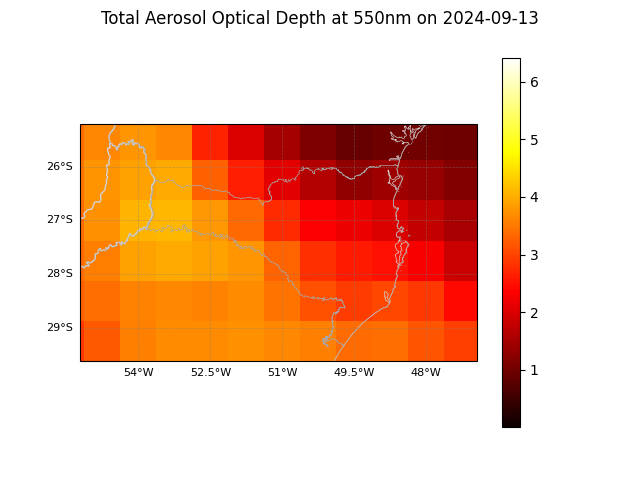
\includegraphics[width=\textwidth, trim=0cm 0cm 0cm 1cm, clip]{images/aod550_2024-09-13_regiao.png}
		\caption{AOD Total - 2024-09-13}
		\label{fig:aod_diario}
	\end{subfigure}
	\hfill
	\begin{subfigure}[b]{0.48\textwidth}
		\centering
		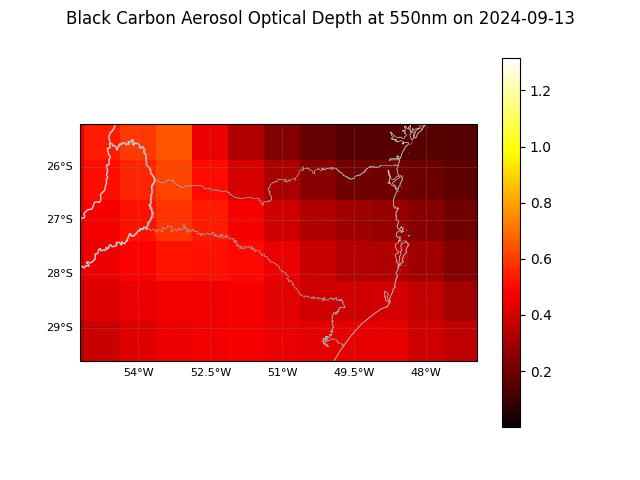
\includegraphics[width=\textwidth, trim=0cm 0cm 0cm 1cm, clip]{images/bcaod550_2024-09-13_regiao.png}
		\caption{Black Carbon AOD - 2024-09-13}
		\label{fig:bcaod_diario}
	\end{subfigure}
	
	\centering
	\begin{subfigure}[b]{0.48\textwidth}
		\centering
		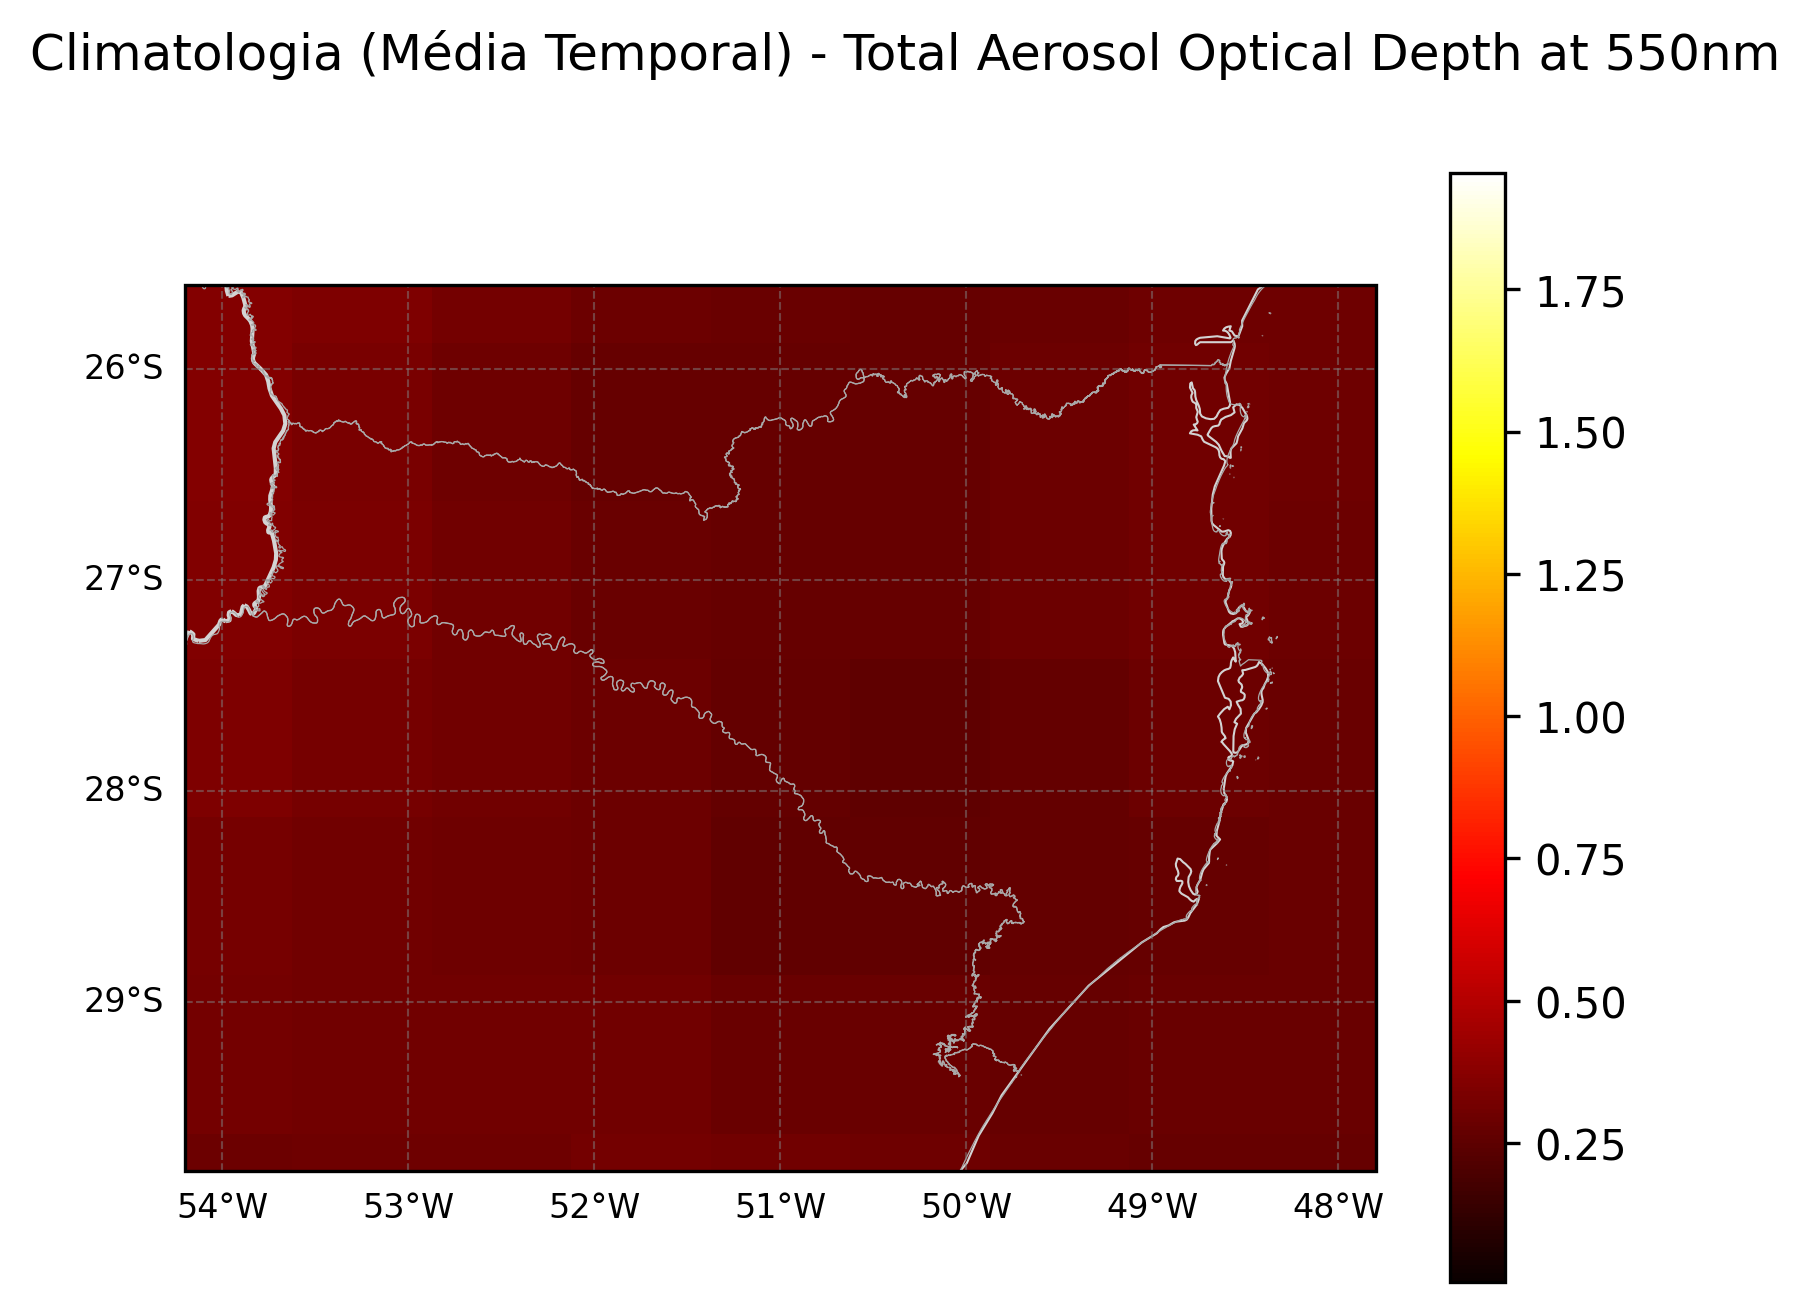
\includegraphics[width=\textwidth, trim=0cm 0cm 0cm 1cm, clip]{images/aod550_climatologia_regiao.png}
		\caption{AOD Total - Média para setembro}
		\label{fig:aod_clima}
	\end{subfigure}
	\hfill
	\begin{subfigure}[b]{0.48\textwidth}
		\centering
		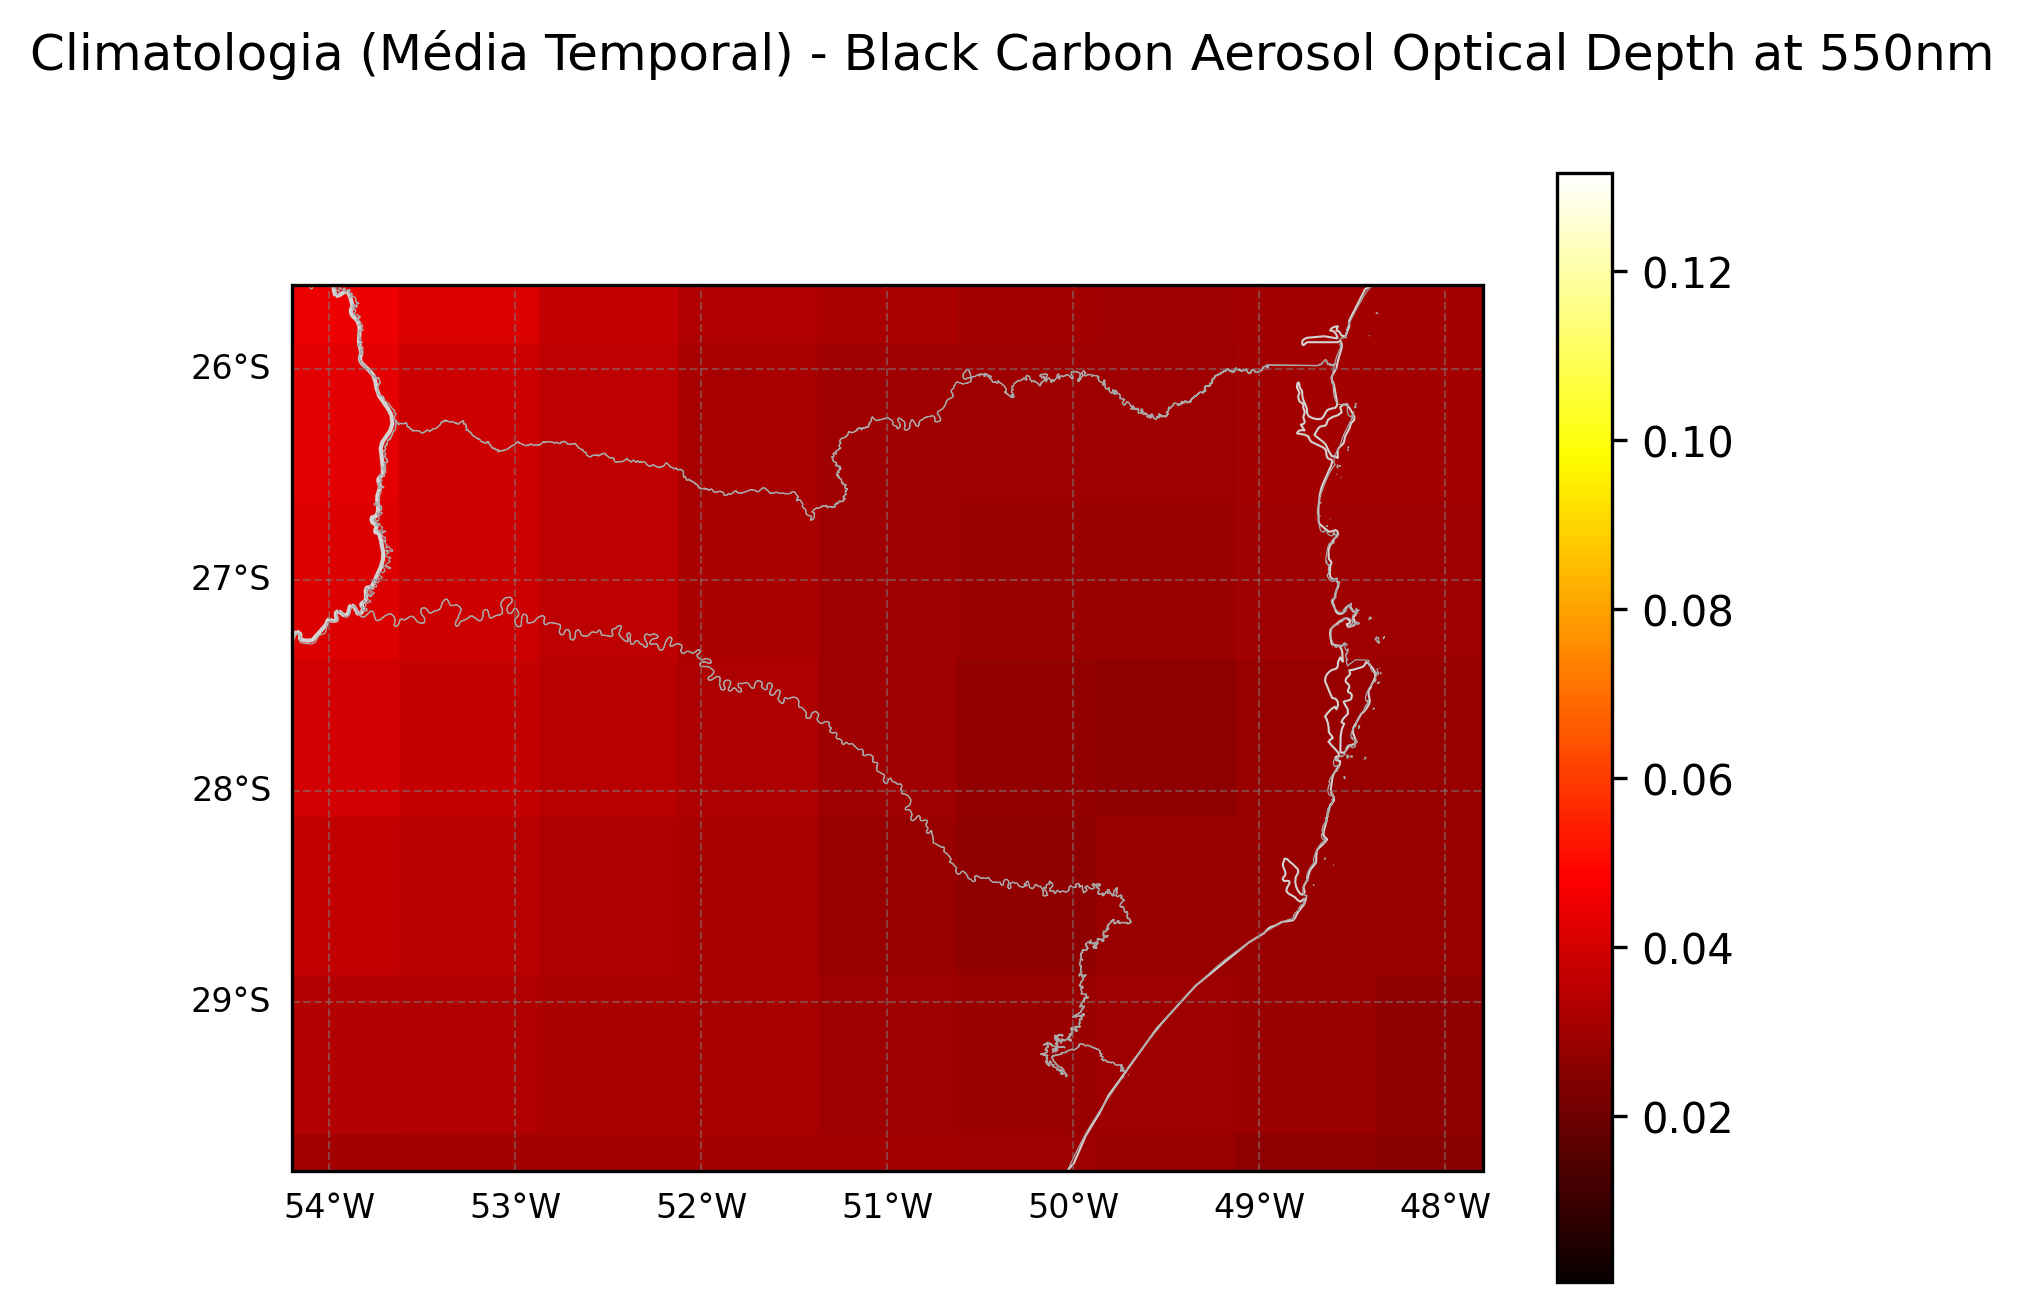
\includegraphics[width=\textwidth, trim=0cm 0cm 0cm 1cm, clip]{images/bcaod550_climatologia_regiao.png}
		\caption{Black Carbon AOD - Média para setembro}
		\label{fig:bcaod_clima}
	\end{subfigure}
	
	\caption{Profundidades Ópticas em 550nm (a) total e (b) específica de Black Carbon sobre o estado de Santa Catarina em 13 de setembro de 2024. Média mensal para setembro de profundidades ópticas em 550nm (c) total e (d) específica de Black Carbon sobre o estado de Santa Catarina entre os anos de 2003 e 2023. Elaboração do autor com dados da reanálise CAMS EAC4.}
	\label{fig:aod_diario_conjunto}
\end{figure}

Assumindo o dia 13 como ponto de referência, foi analisado o perfil da atmosfera nos dias que antecederam essa data. Entre as Figuras \ref{fig:sinotica_20240905_1200} e \ref{fig:sinotica_20240913_1200} estão dispostos mapas de variáveis meteorológicas para a América do Sul entre os dias 05 e 13 de setembro de 2024. É possível identificar um sistema de alta pressão em superfície posicionado próximo à latitude de 40°S, tanto pelos valores de pressão a nível médio do mar e escoamento a 10m, quanto pelos gradientes de temperatura do ponto de orvalho. Entre os 8 dias analisados, o deslocamento desse sistema para oeste se deu entre 140° e 120° O. Ao longo do nível de 500 hPa, identifica-se um cavado à frente do sistema de alta anteriormente identificado, o que corrobora com um bloqueio de tipo ômega citado na seção \ref{sec:bloqueio}. 

Na Figura \ref{fig:goesgeral}, estão dispostas as imagens geradas pelo canal 13 do satélite GOES16, onde as cores mais quentes significam topos de nuvens mais altos, ou seja, maior atividade convectiva ocorrendo naquele local. Ao longo do período analisado, não foram identificados padrões de nuvens que se assemelhem à passagem de sistemas frontais pela região sul do Brasil após o dia 05 de setembro.



\begin{figure}[htb]
	\centering	
	\begin{subfigure}[b]{\textwidth}
		\centering
		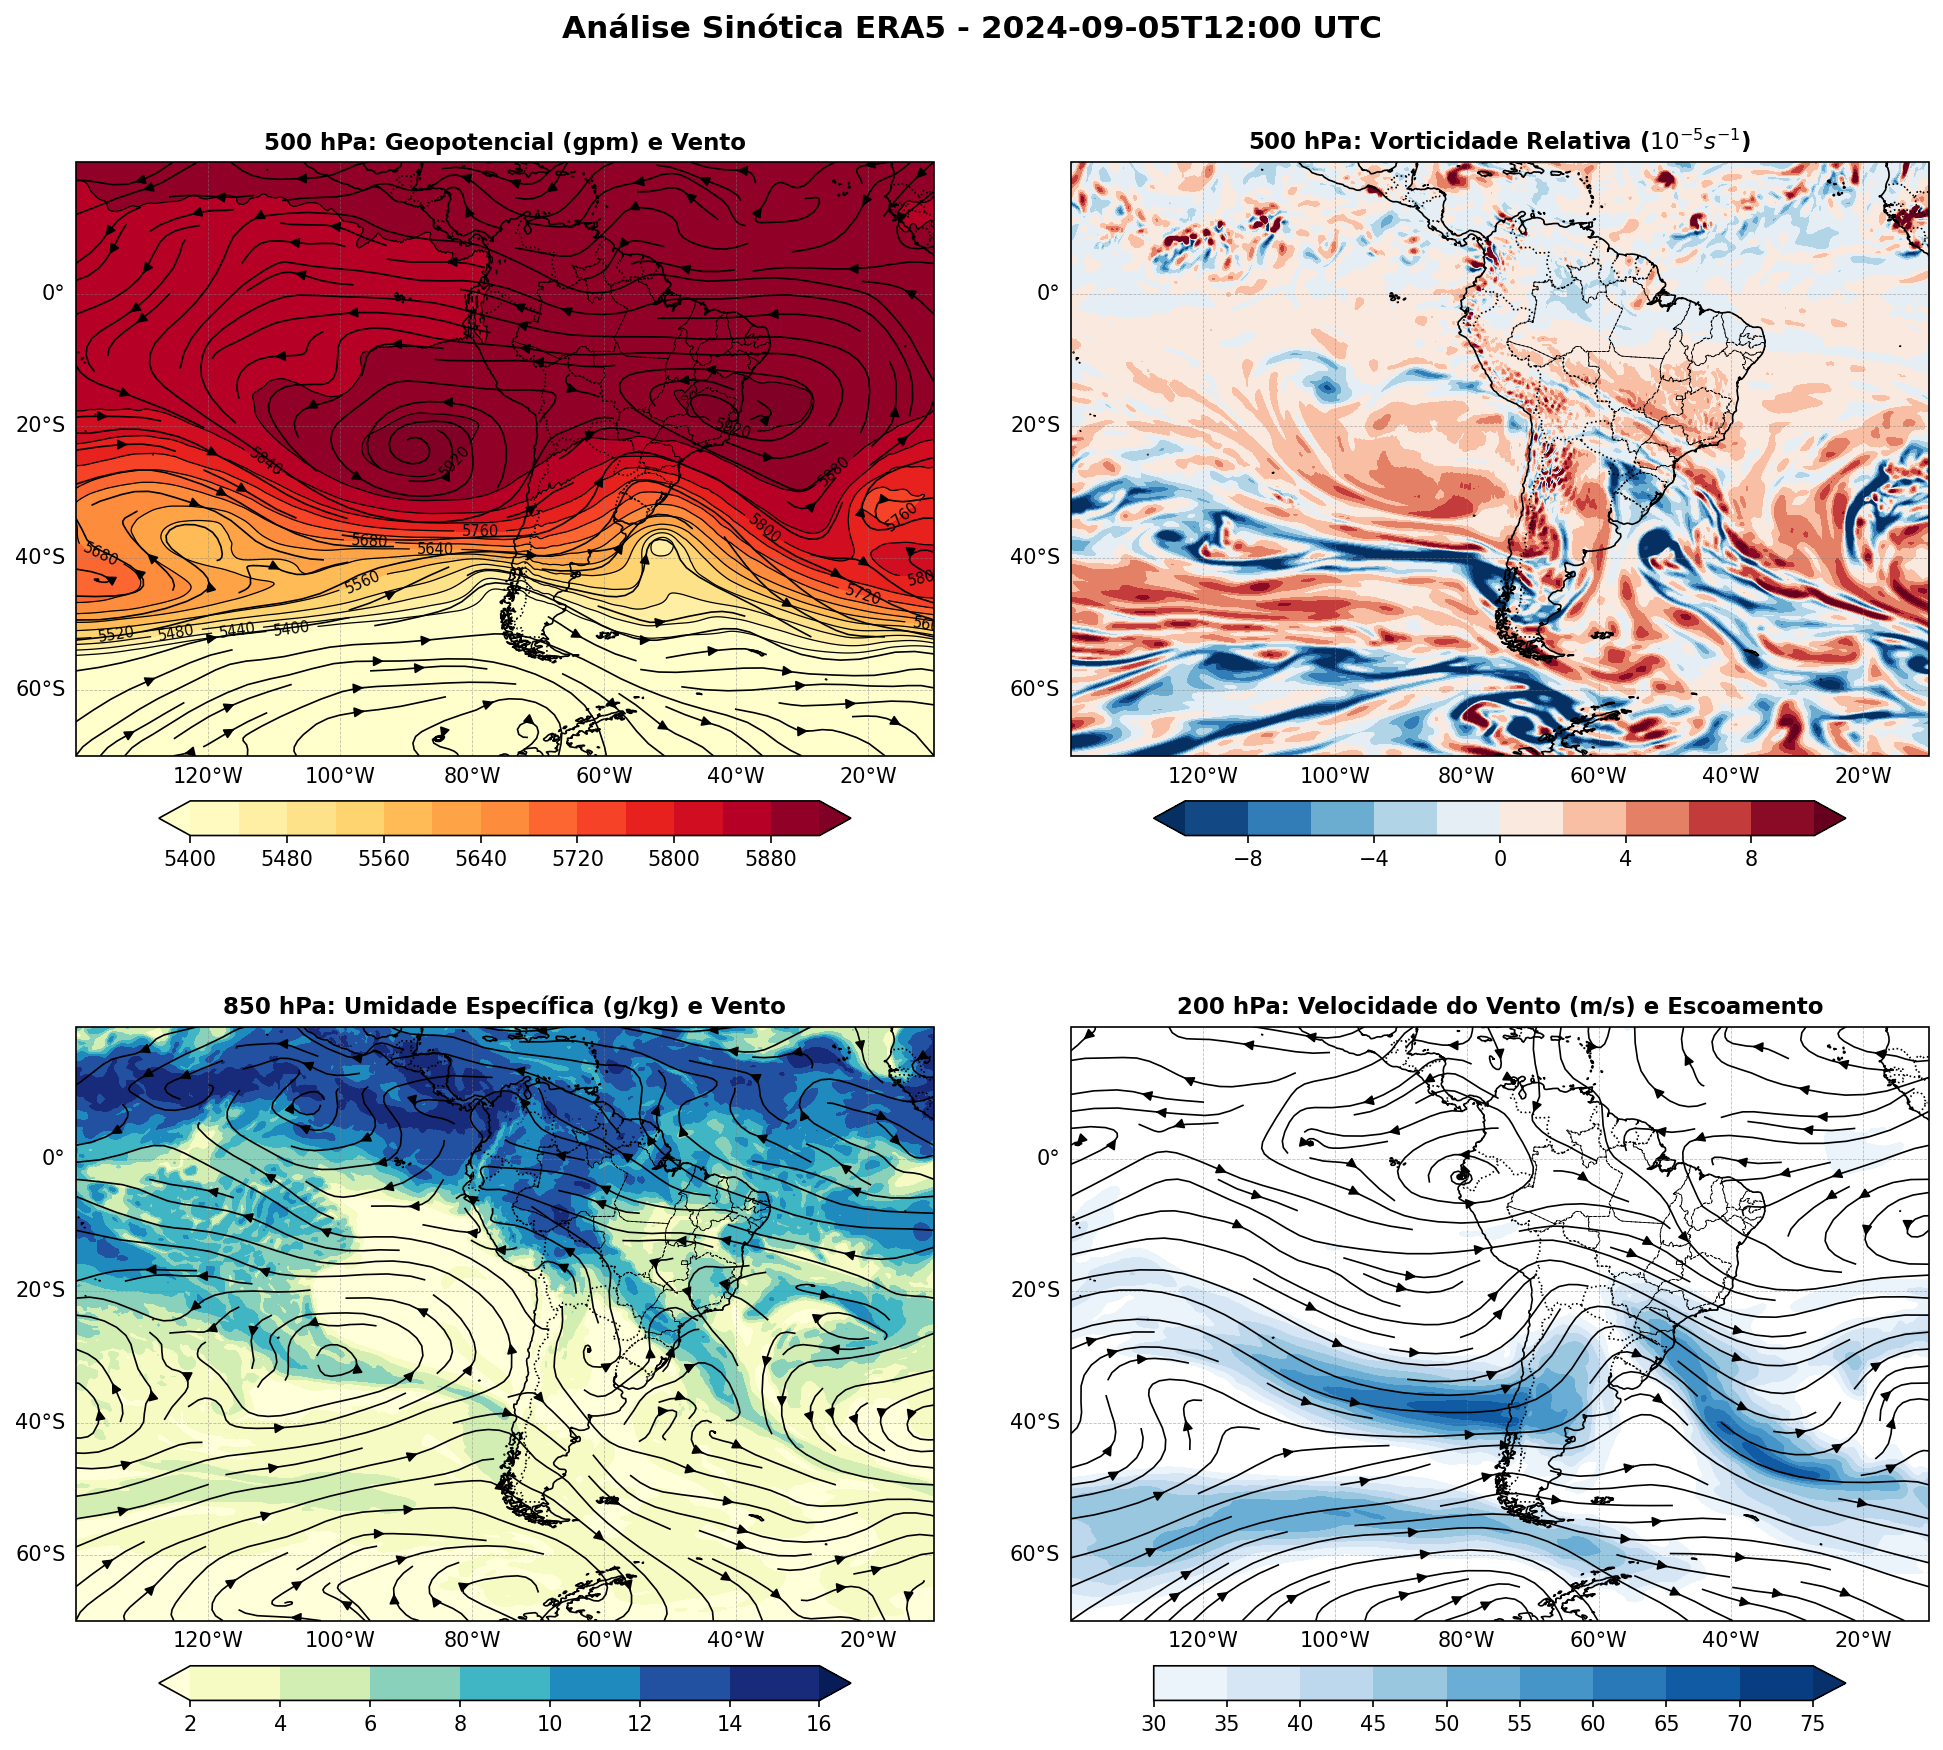
\includegraphics[width = 0.48\textwidth, trim=0cm 0cm 0cm 2cm, clip]{images/sinotica_20240905_1200.png}
		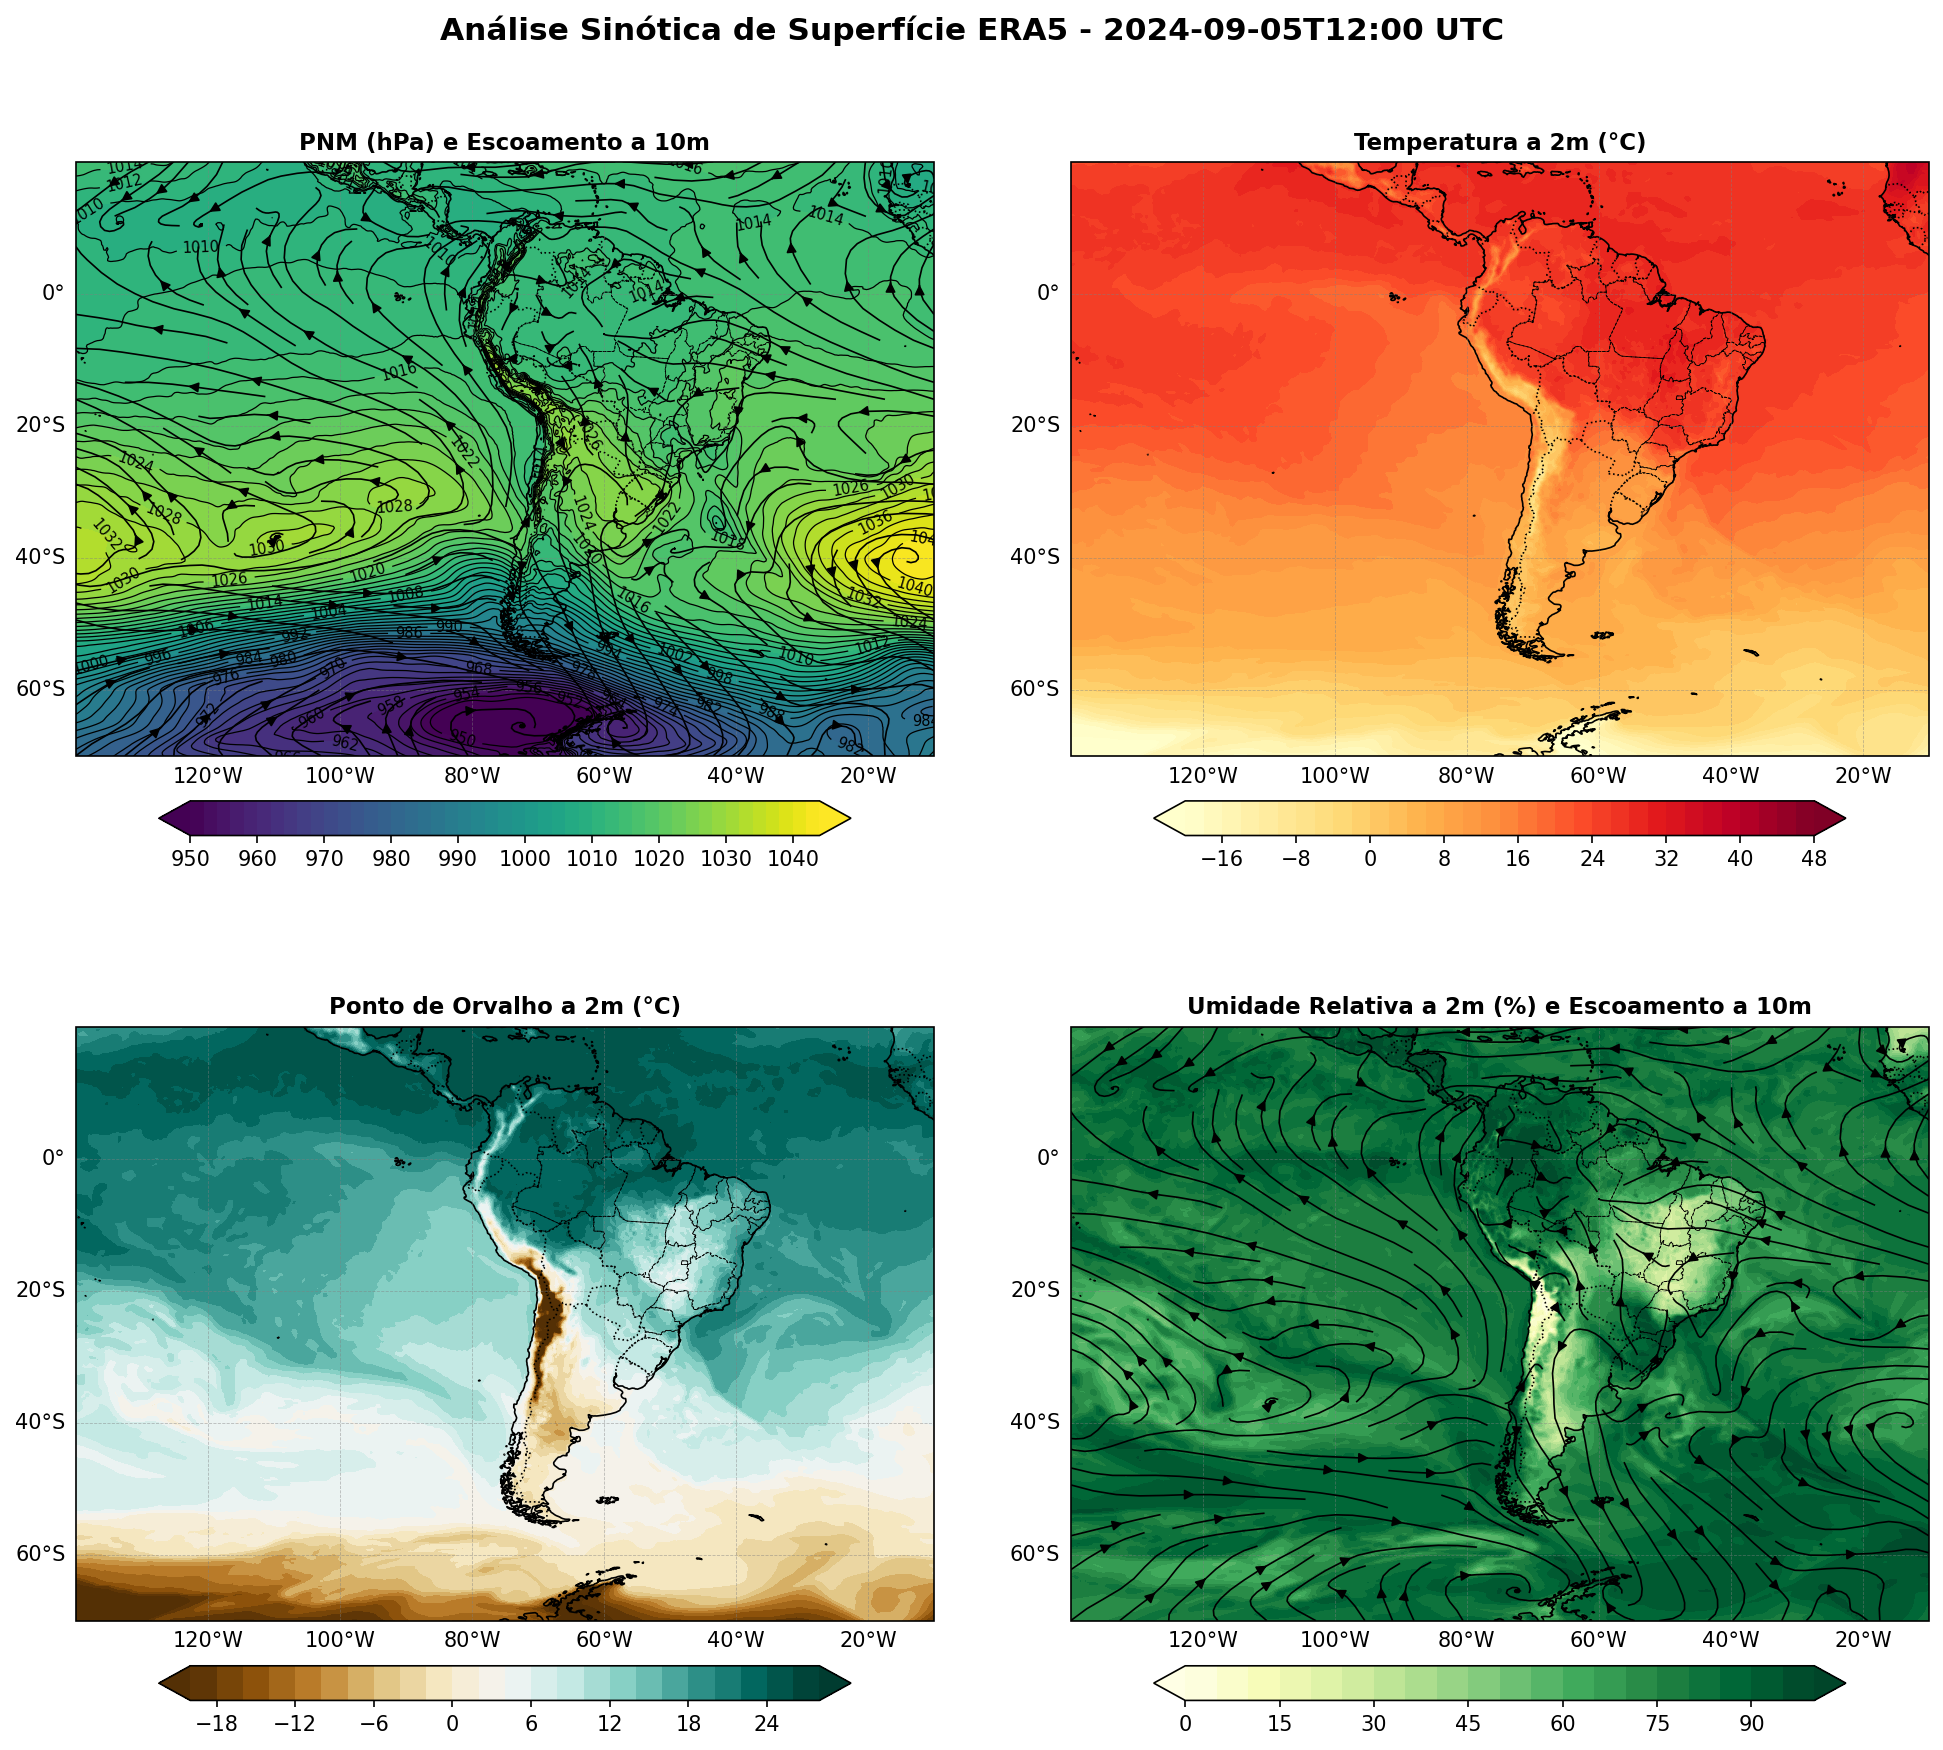
\includegraphics[width = 0.48\textwidth, trim=0cm 0cm 0cm 2cm, clip]{images/superficie_20240905_1200.png}
	\end{subfigure}
		\caption{Análise Sinótica ERA5 - 2024-09-05T12:00 UTC}
		\label{fig:sinotica_20240905_1200}
\end{figure}


\begin{figure}[htb]
	\centering	
	\begin{subfigure}[b]{\textwidth}
		\centering
		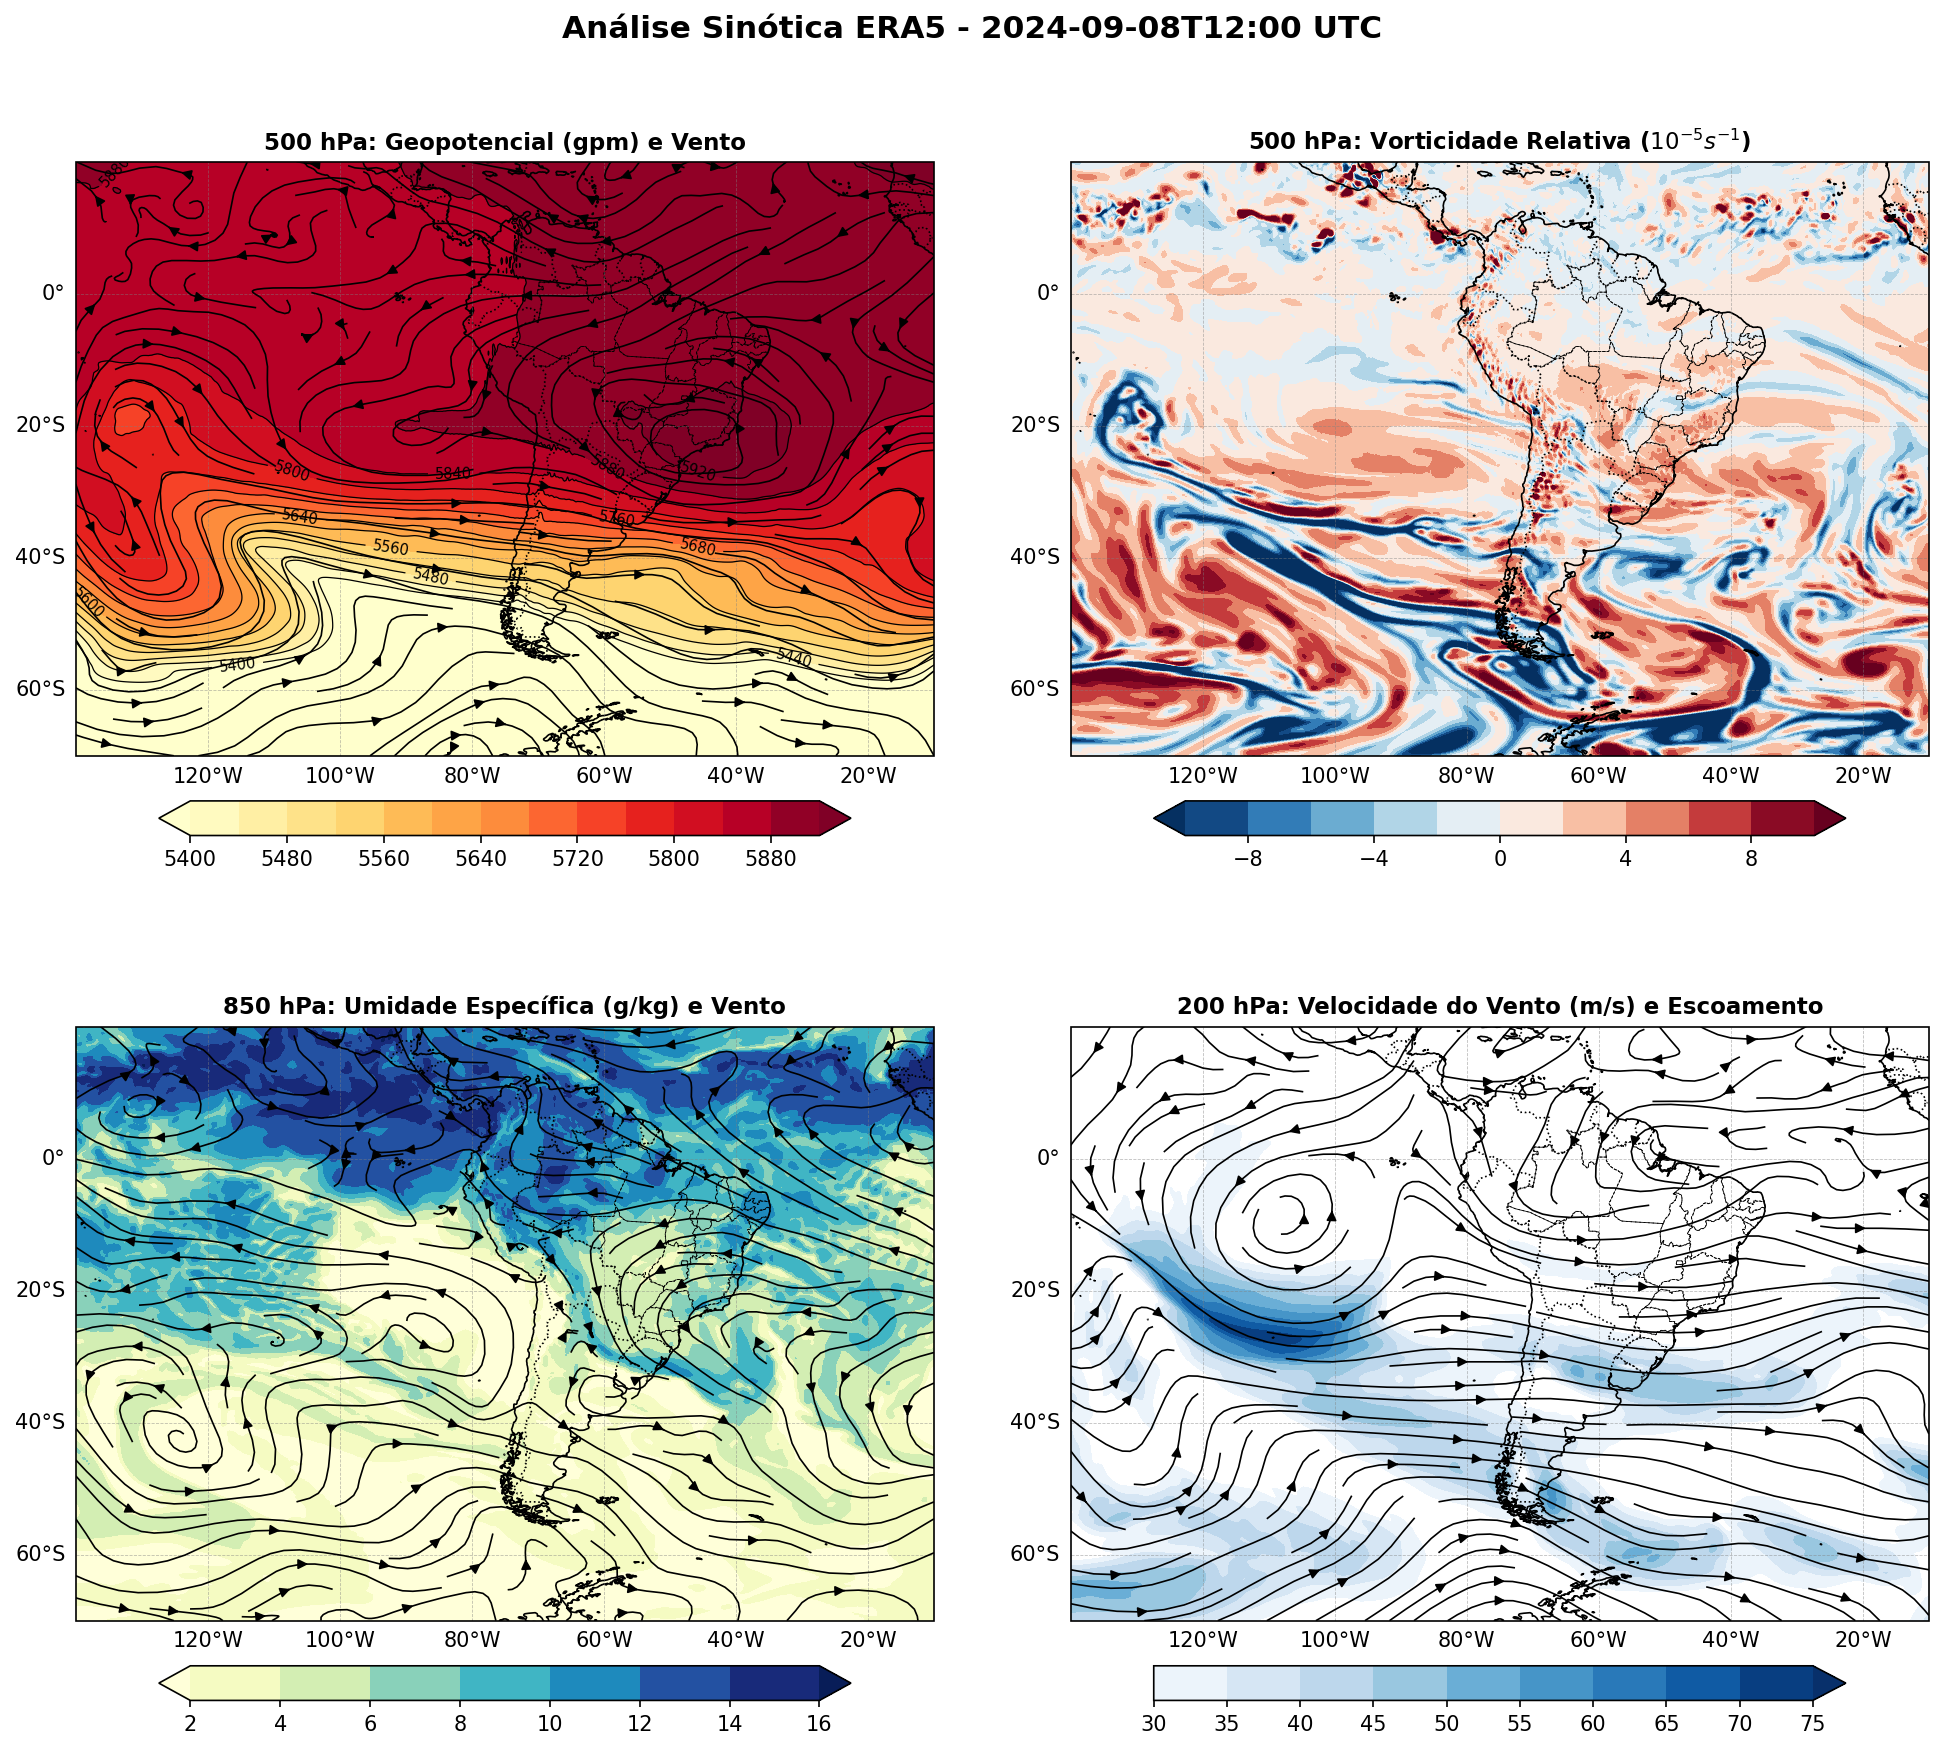
\includegraphics[width = 0.48\textwidth, trim=0cm 0cm 0cm 2cm, clip]{images/sinotica_20240908_1200.png}
		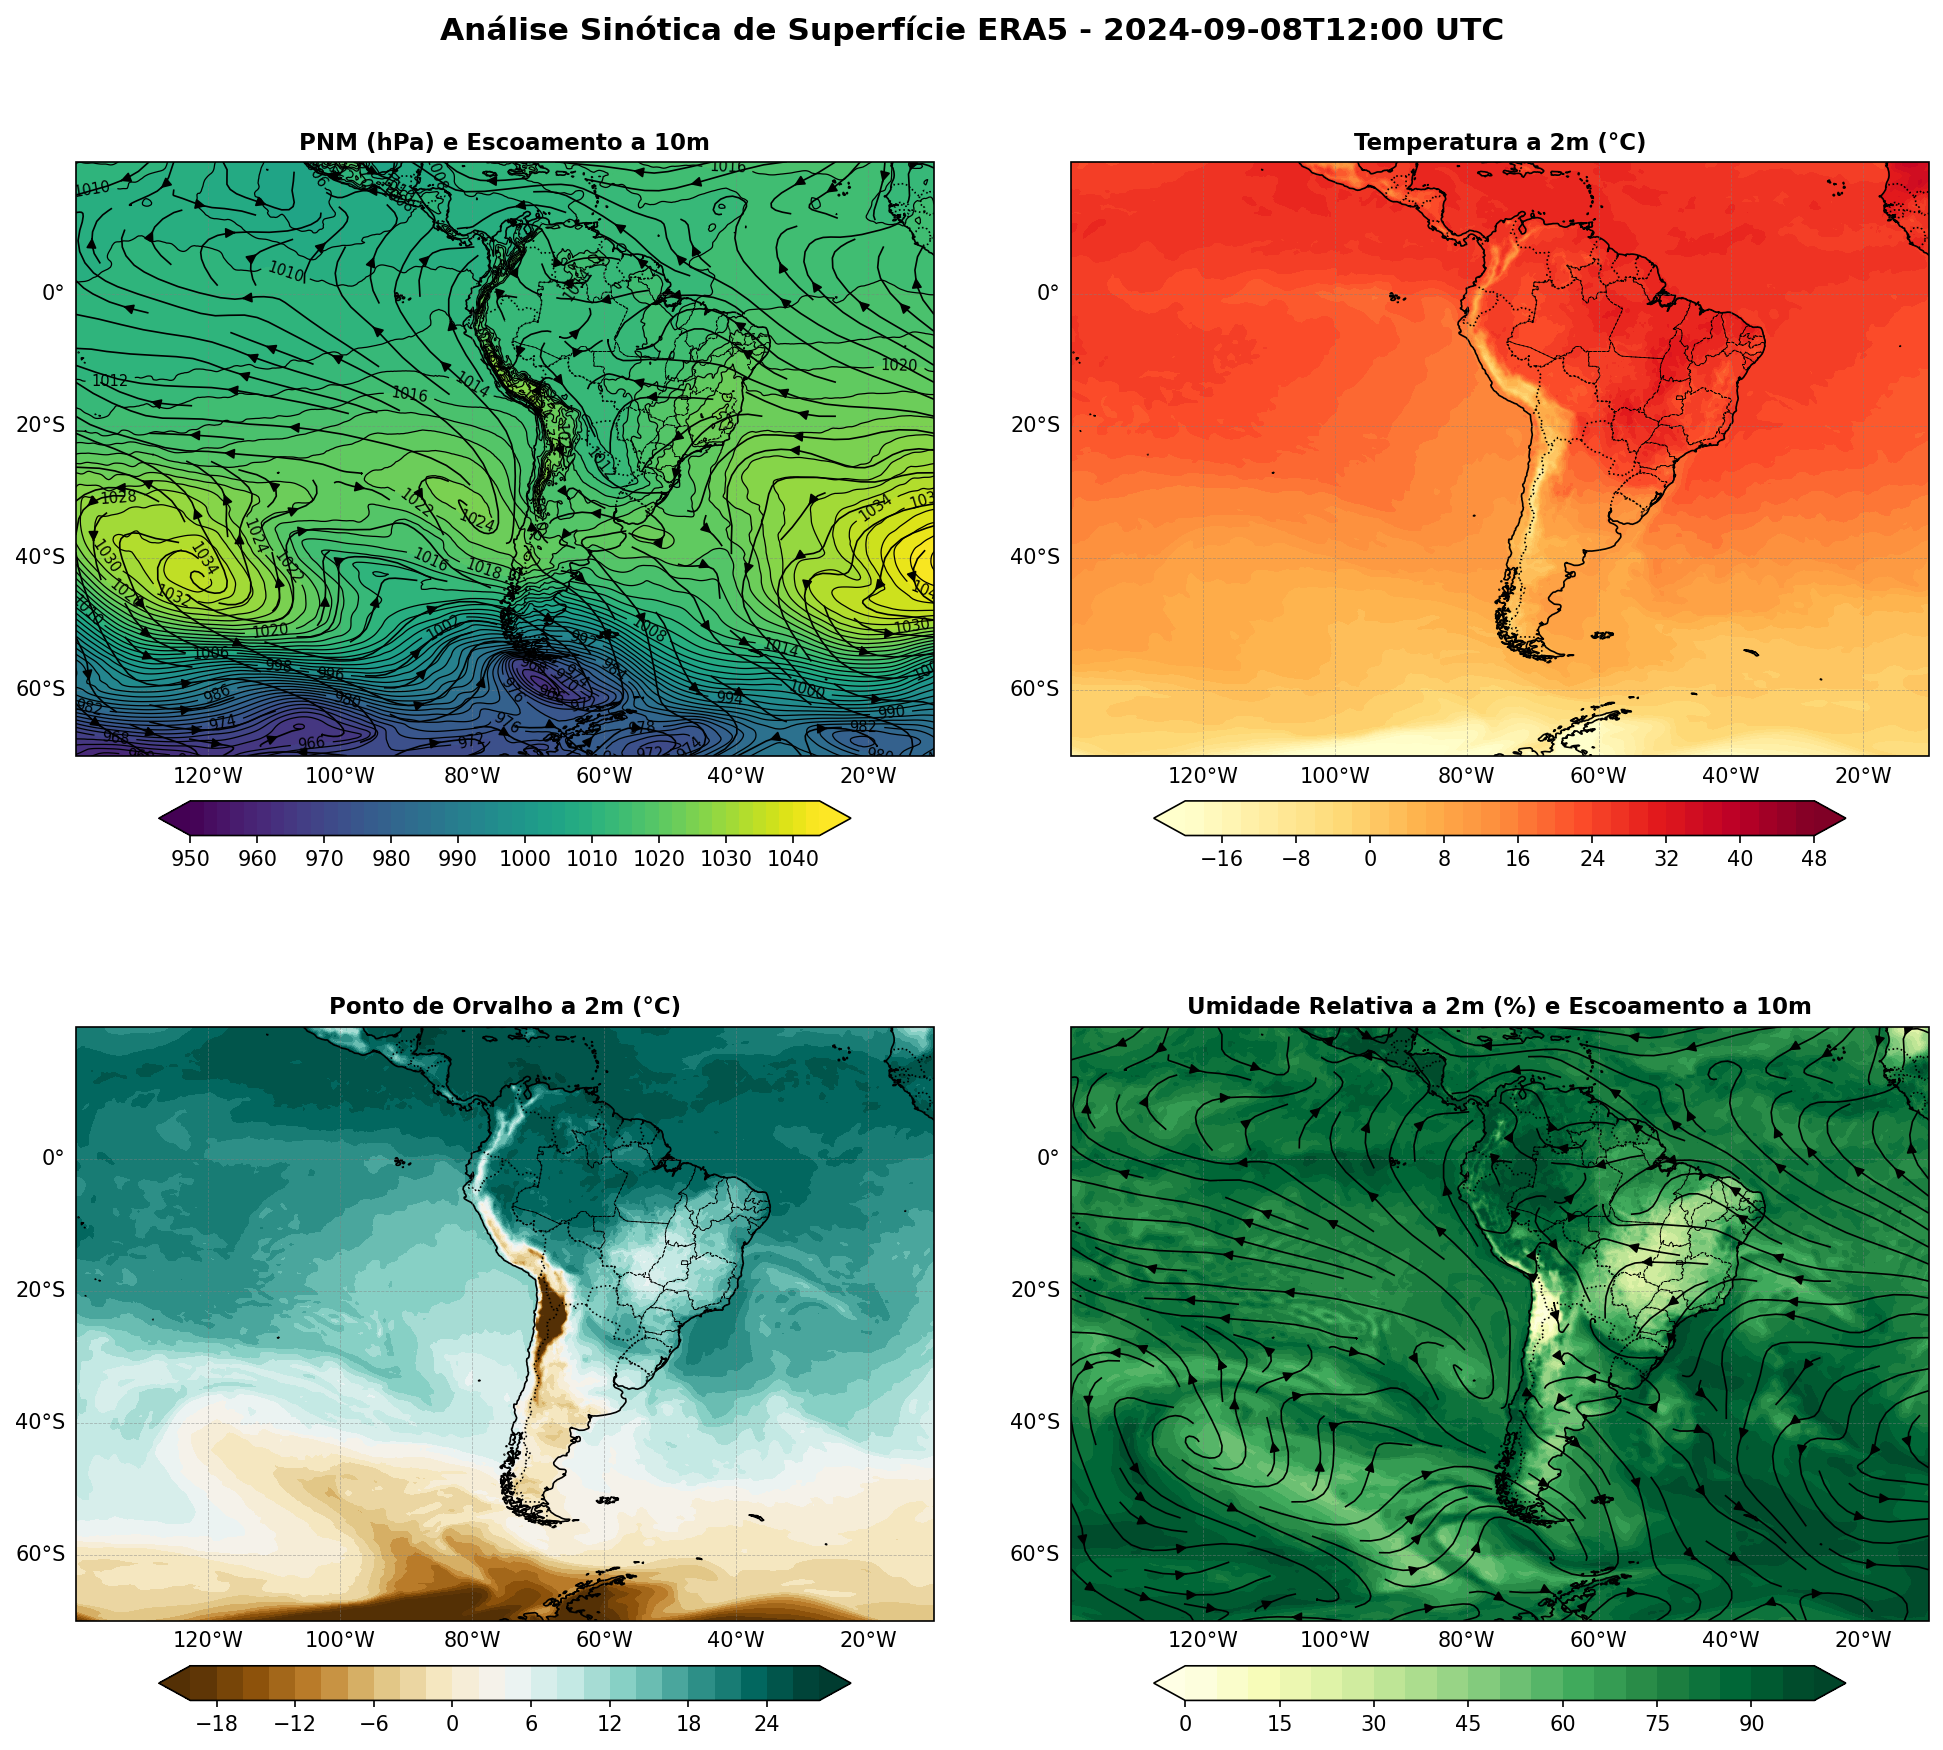
\includegraphics[width = 0.48\textwidth, trim=0cm 0cm 0cm 2cm, clip]{images/superficie_20240908_1200.png}
	\end{subfigure}
	\caption{Análise Sinótica ERA5 - 2024-09-08T12:00 UTC}
	\label{fig:sinotica_20240908_1200}
\end{figure}

\begin{figure}[htb]
	\centering	
	\begin{subfigure}[b]{\textwidth}
		\centering
		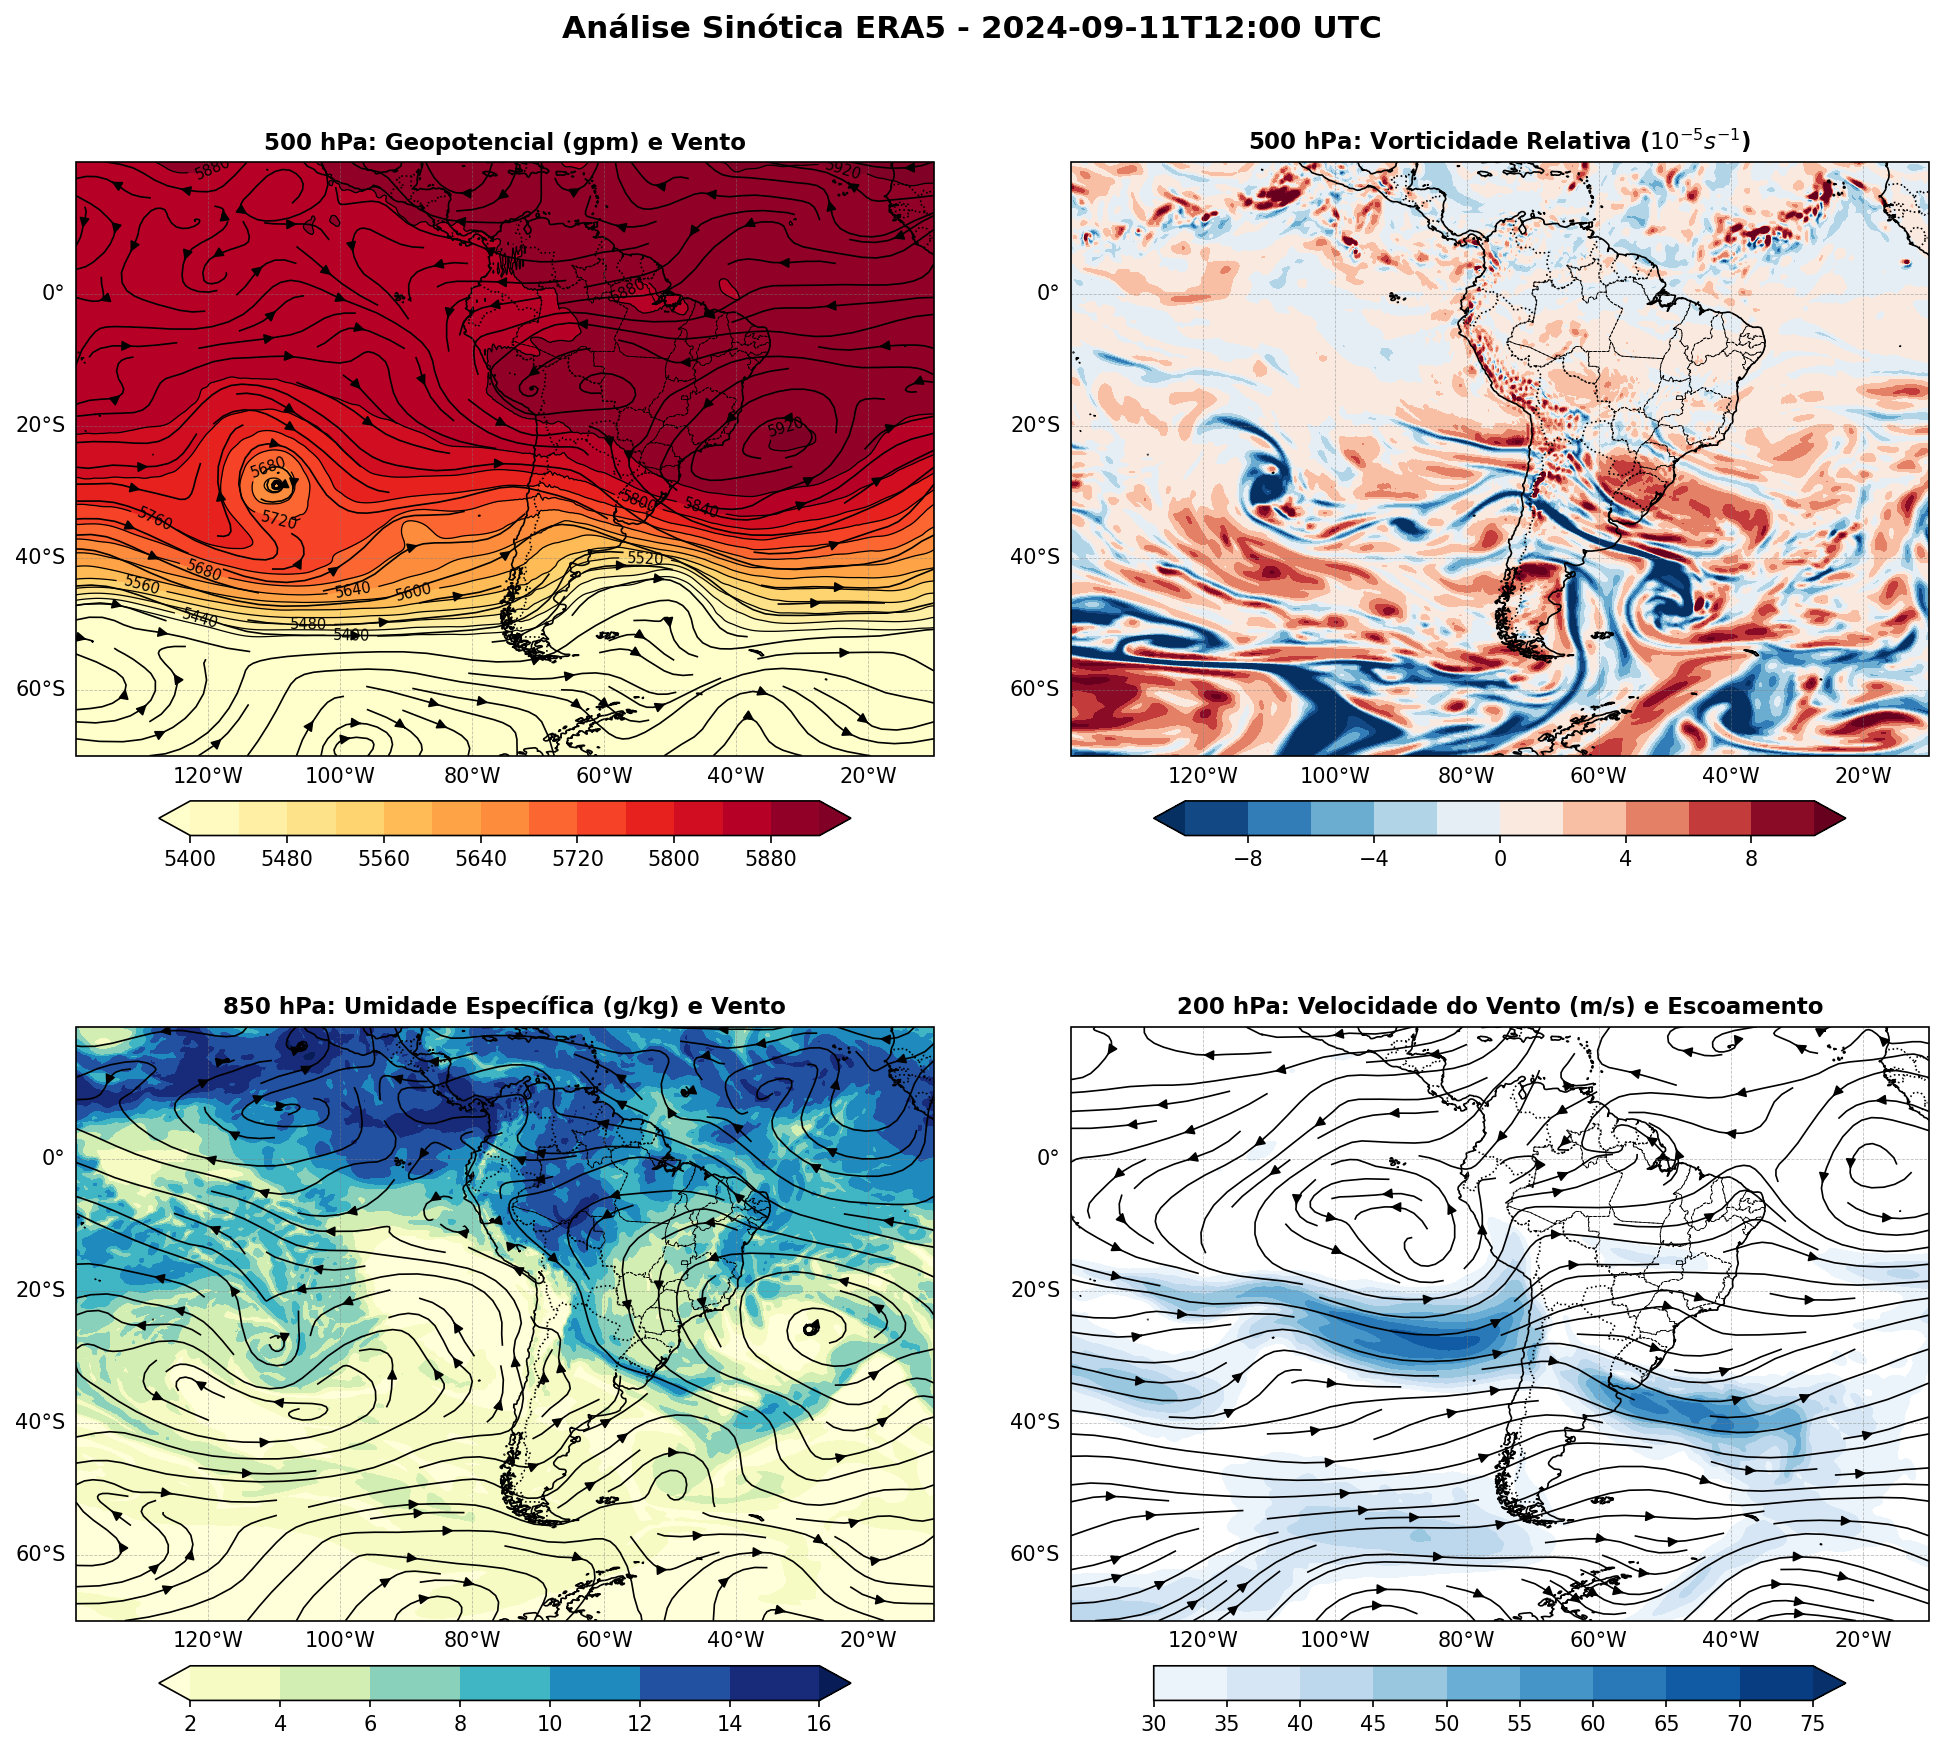
\includegraphics[width = 0.48\textwidth, trim=0cm 0cm 0cm 2cm, clip]{images/sinotica_20240911_1200.png}
		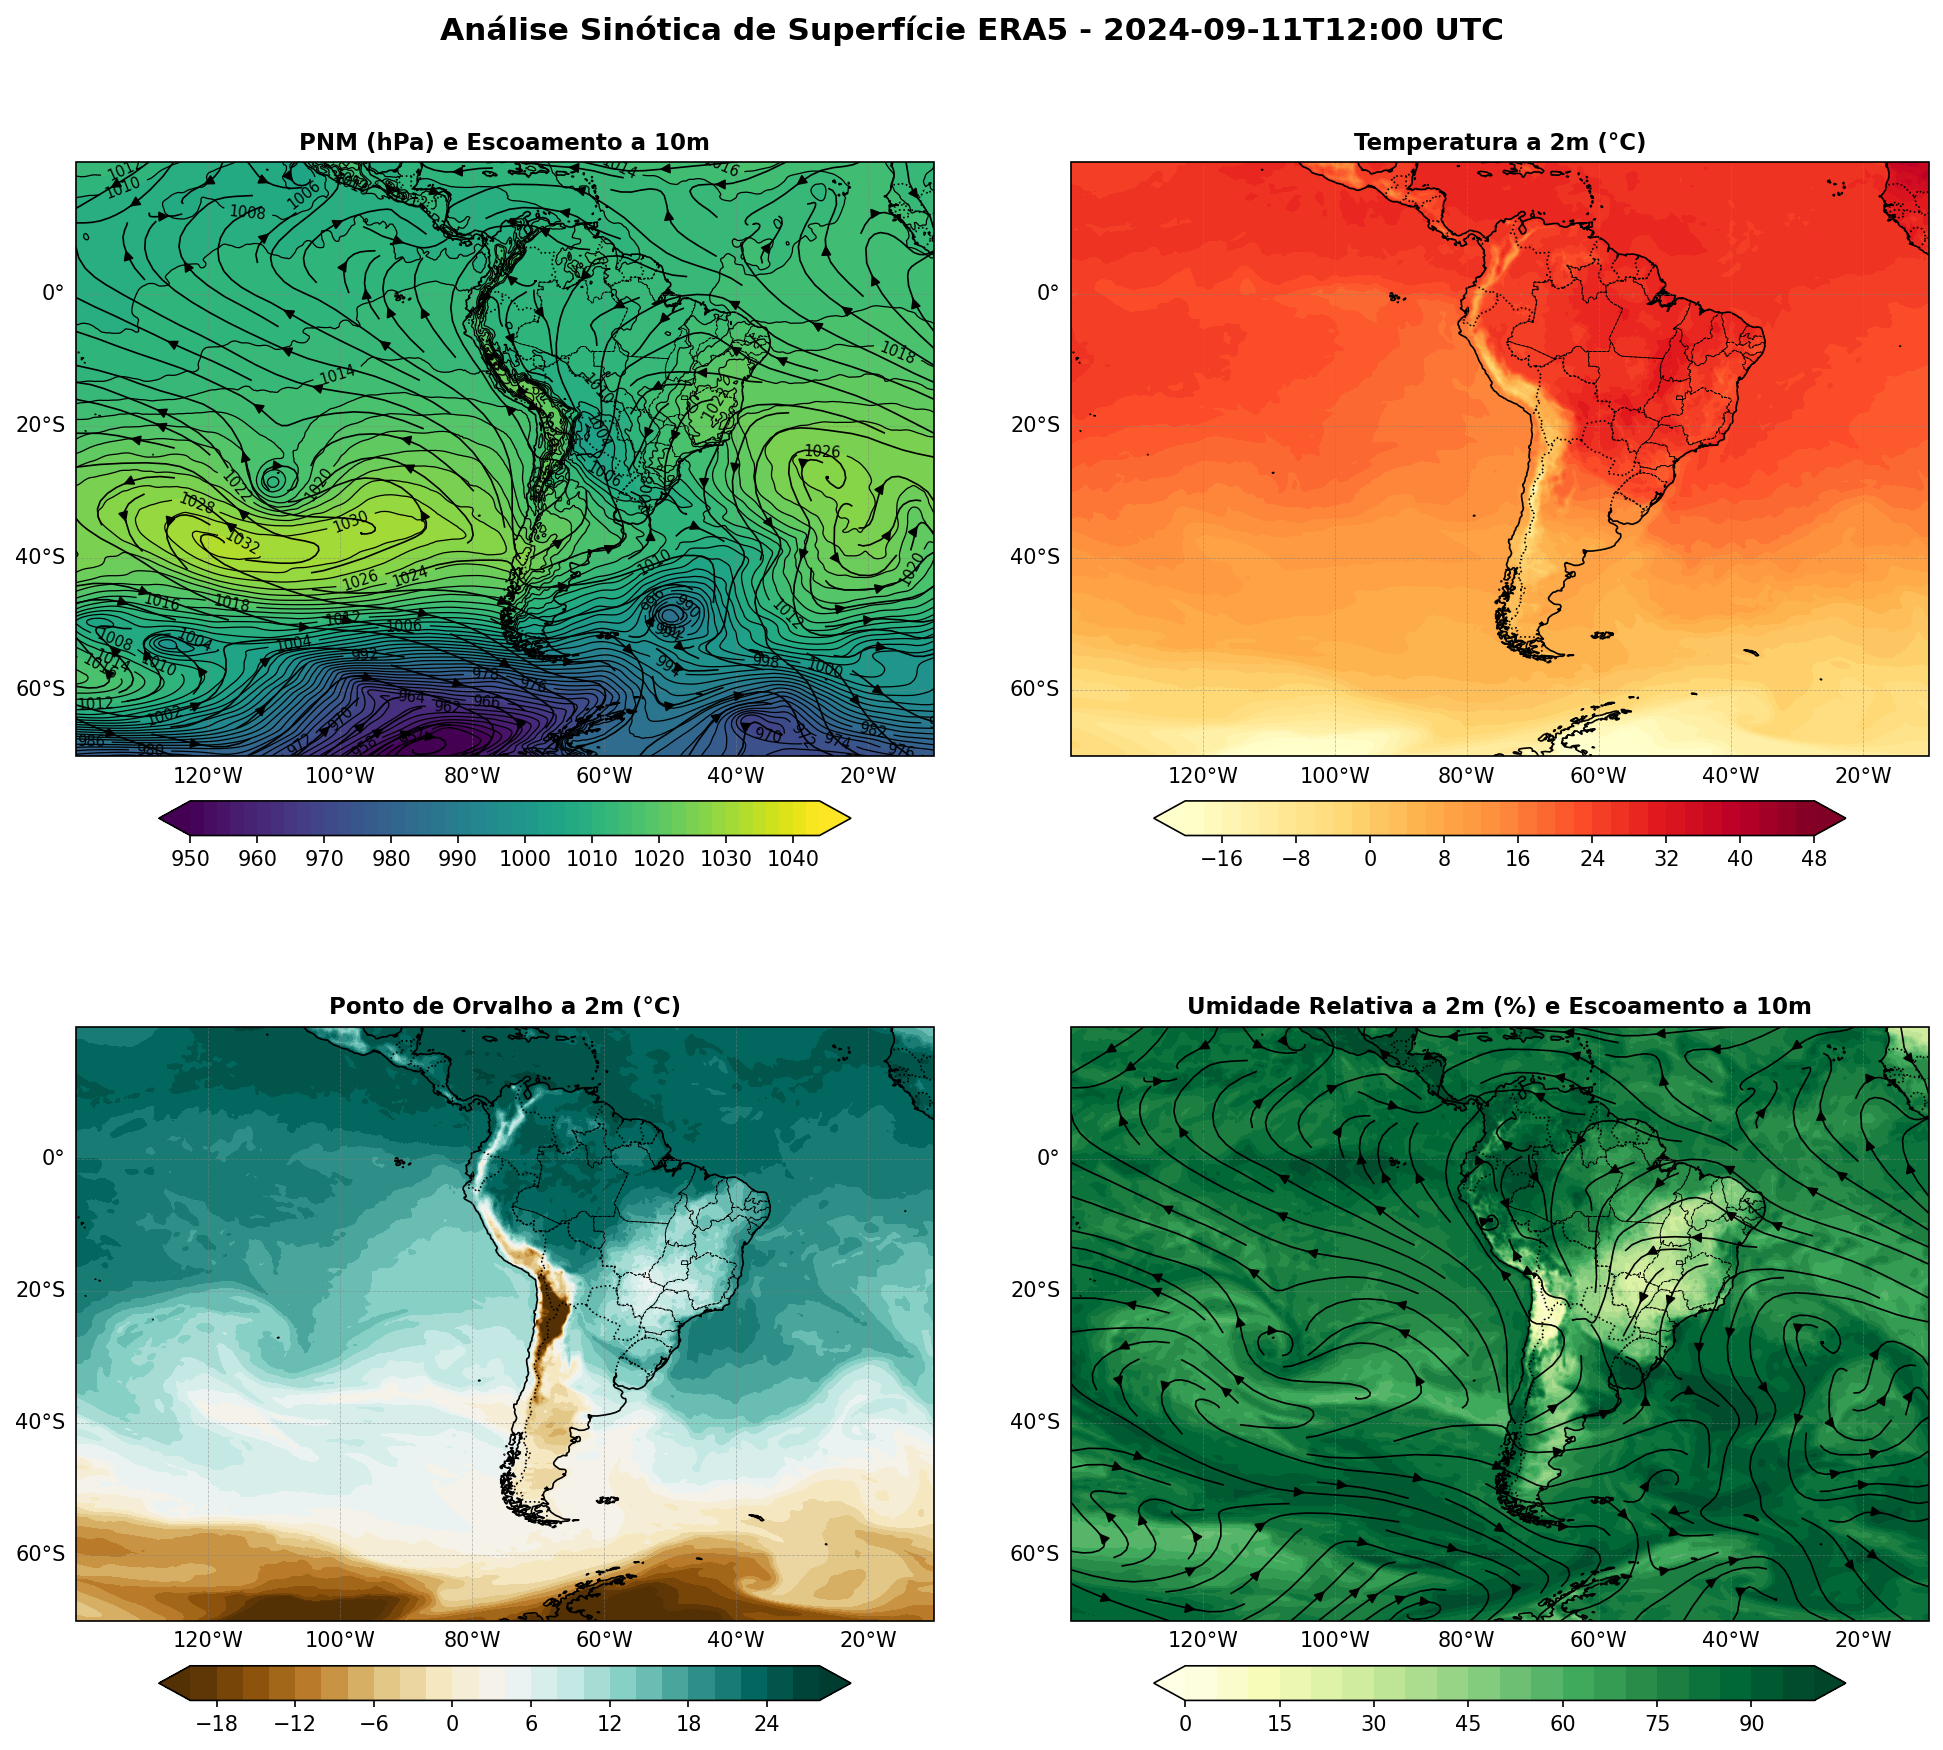
\includegraphics[width = 0.48\textwidth, trim=0cm 0cm 0cm 2cm, clip]{images/superficie_20240911_1200.png}
	\end{subfigure}
	\caption{Análise Sinótica ERA5 - 2024-09-11T11:00 UTC}
	\label{fig:sinotica_20240908_1100}
\end{figure}



\begin{figure}[htb]
	\centering	
	\begin{subfigure}[b]{\textwidth}
		\centering
		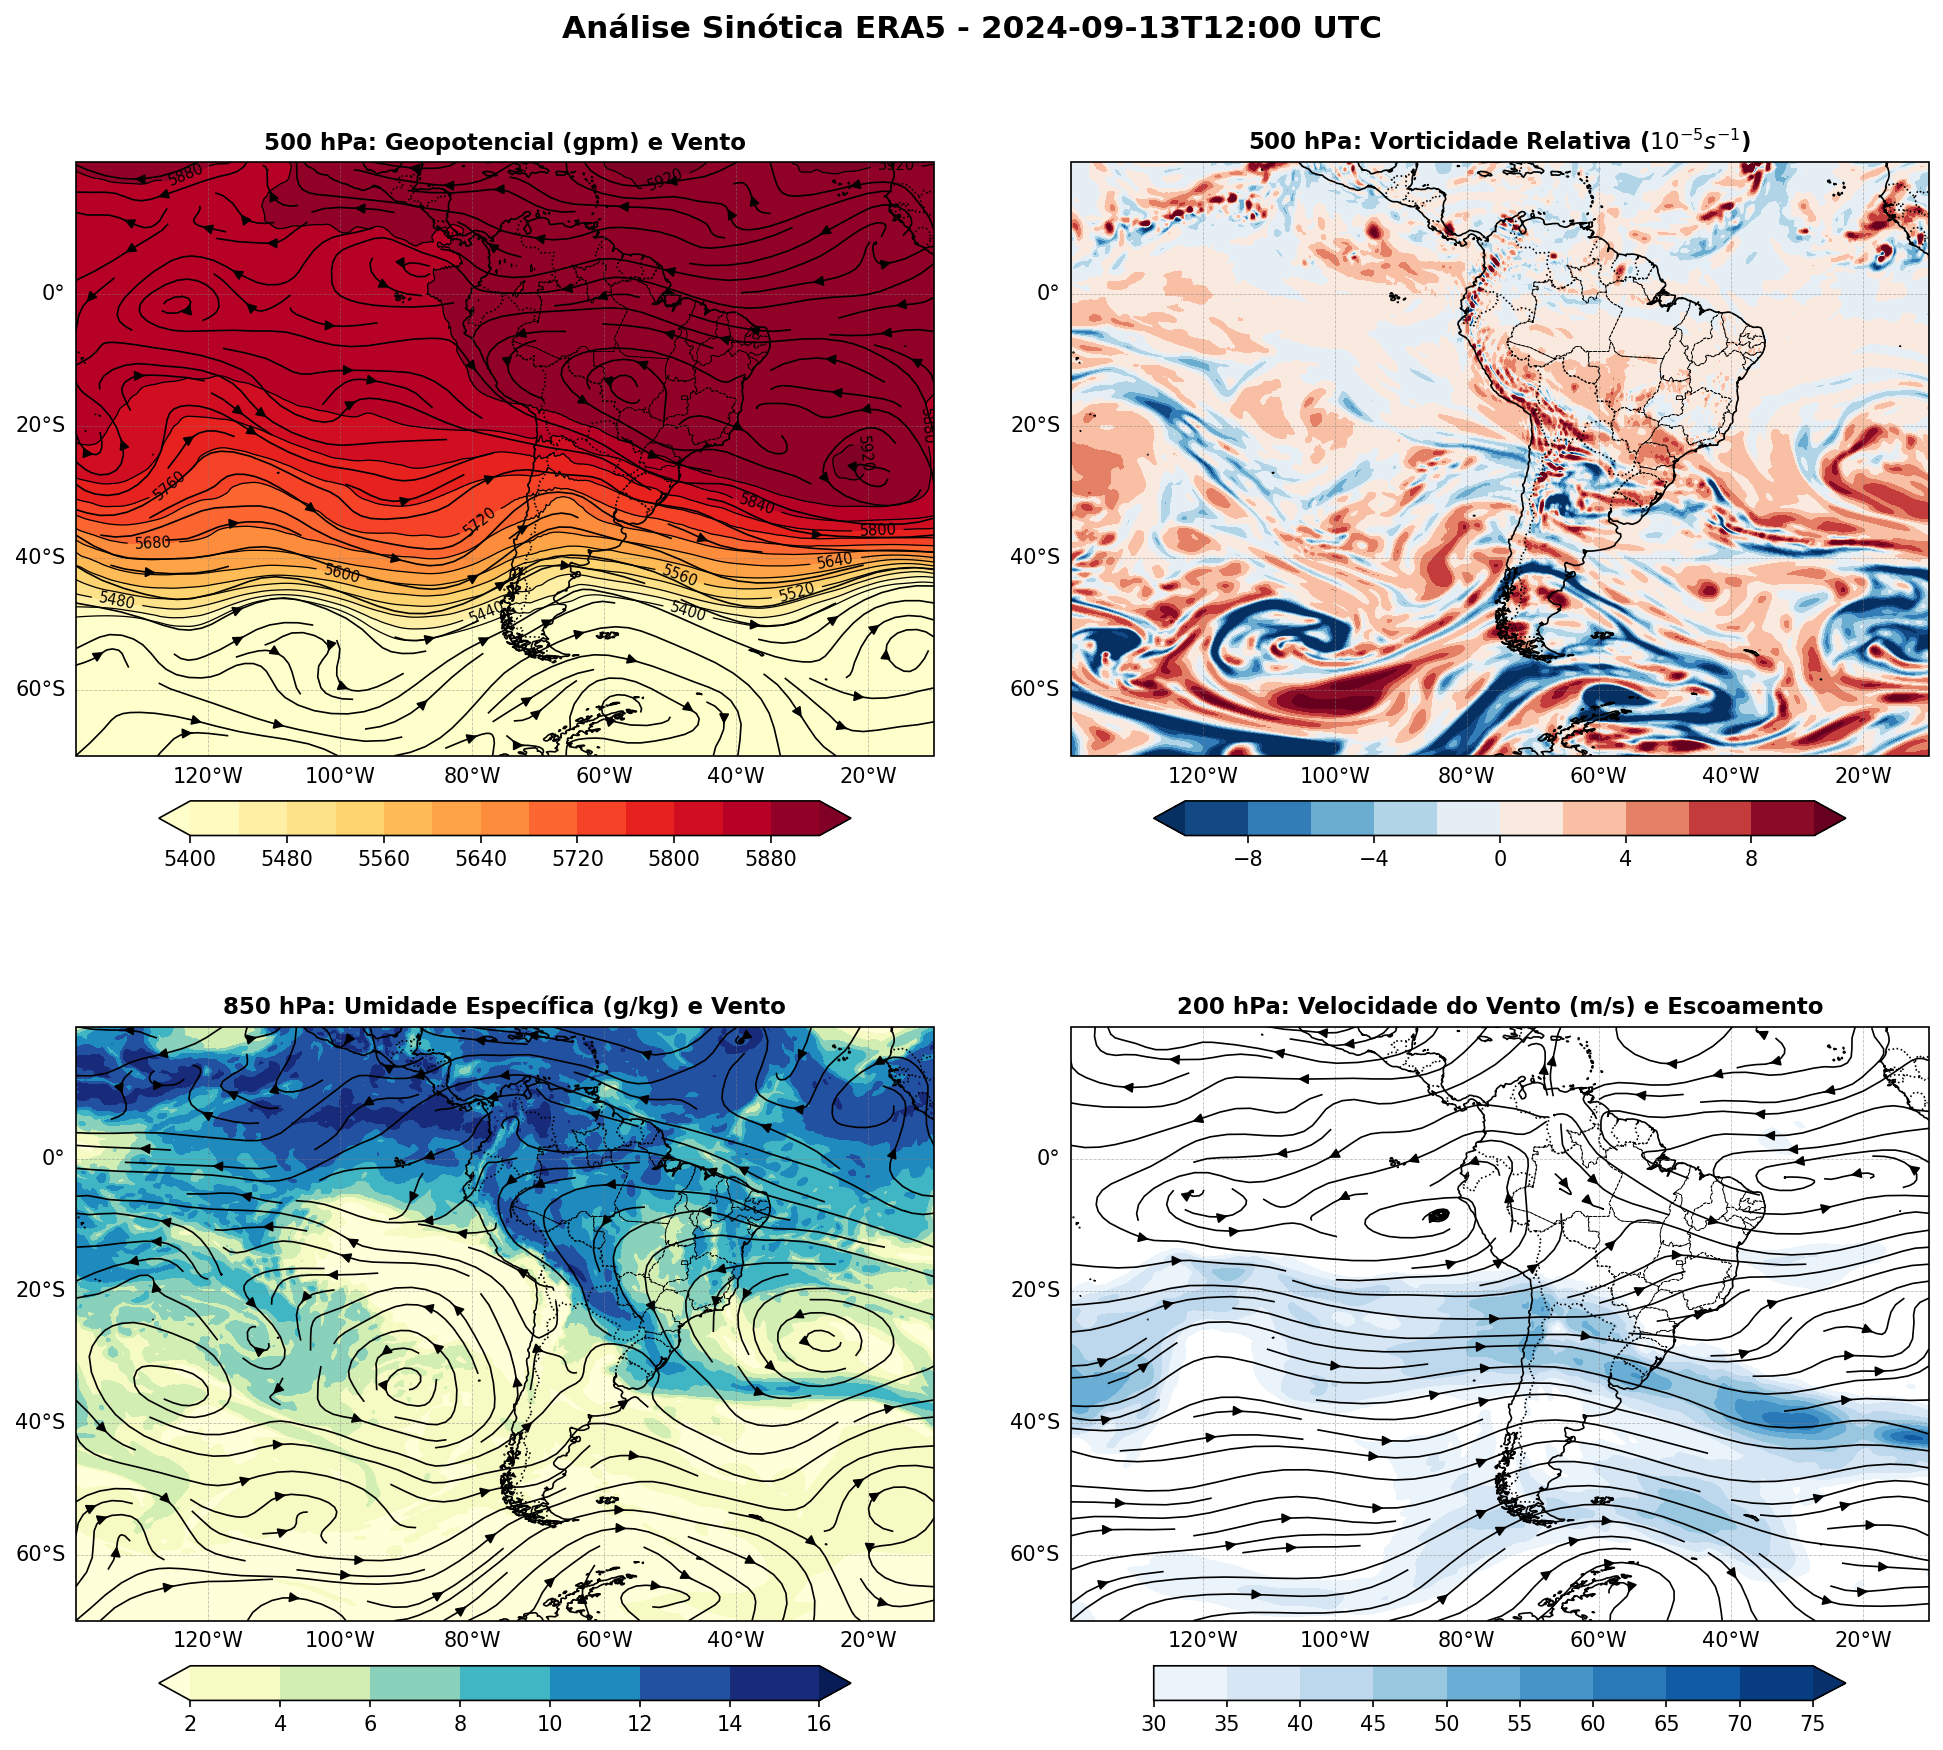
\includegraphics[width = 0.48\textwidth, trim=0cm 0cm 0cm 2cm, clip]{images/sinotica_20240913_1200.png}
		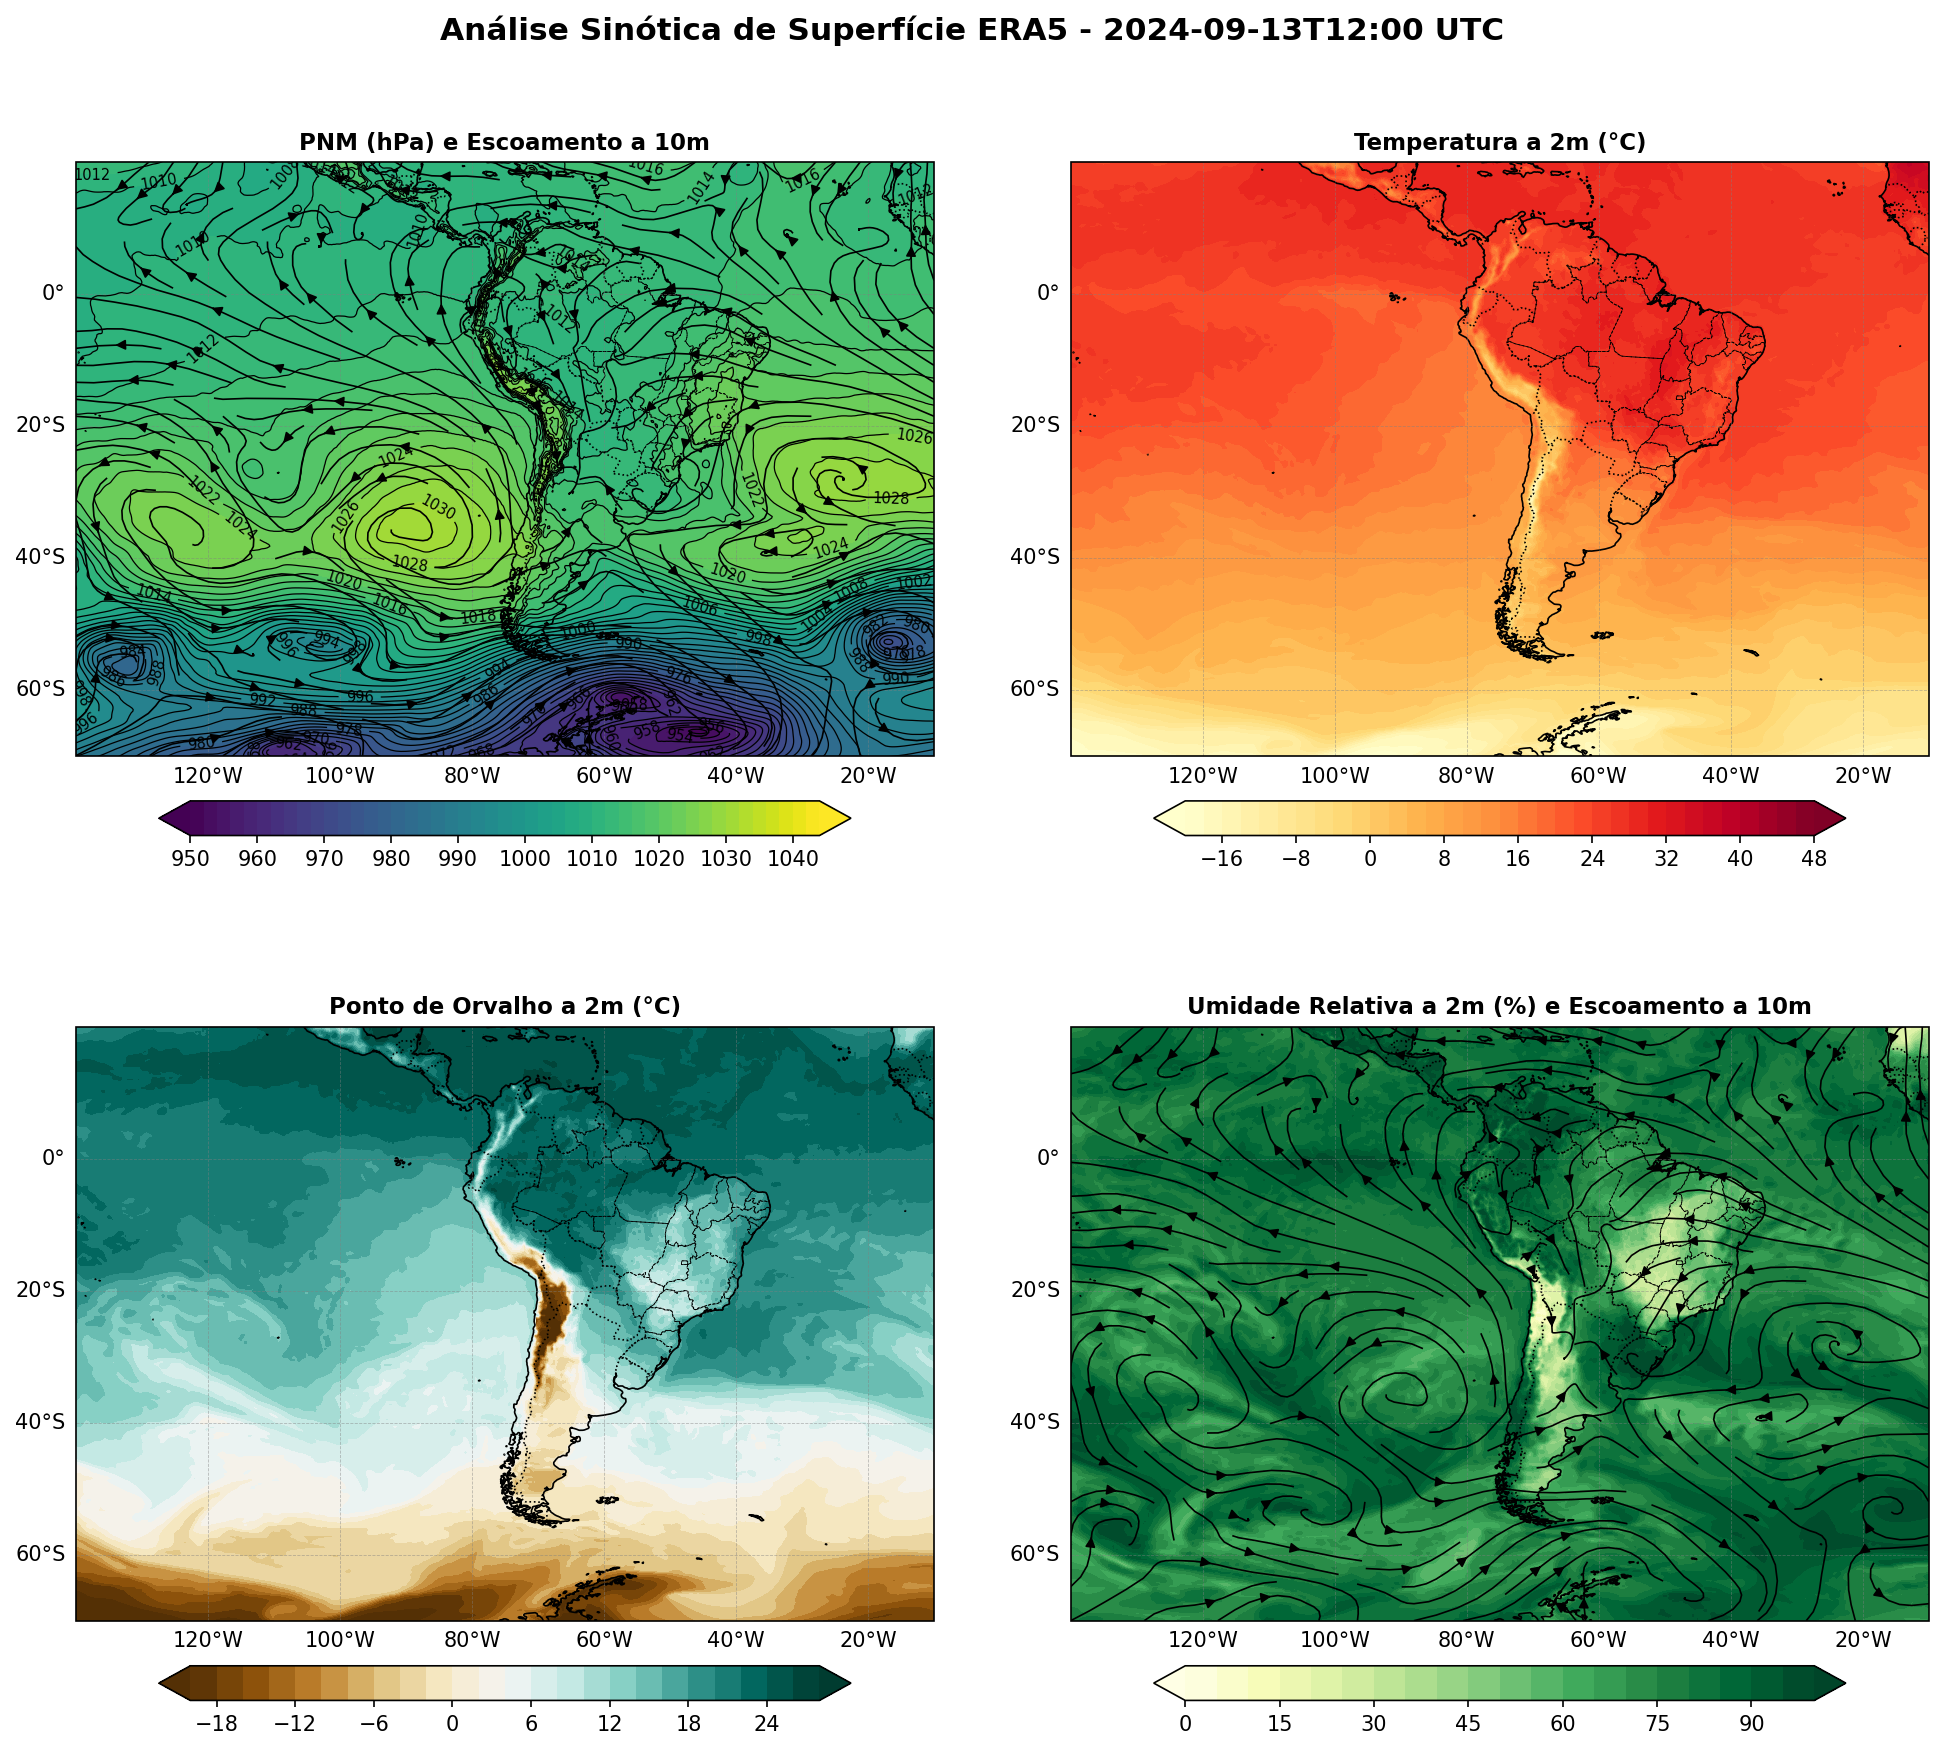
\includegraphics[width = 0.48\textwidth, trim=0cm 0cm 0cm 2cm, clip]{images/superficie_20240913_1200.png}
	\end{subfigure}
	\caption{Análise Sinótica ERA5 - 2024-09-13T12:00 UTC}
	\label{fig:sinotica_20240913_1200}
\end{figure}


\begin{figure}
		\centering
	% --- LINHA 1 ---
	\begin{subfigure}[b]{0.4\textwidth}
	\centering
	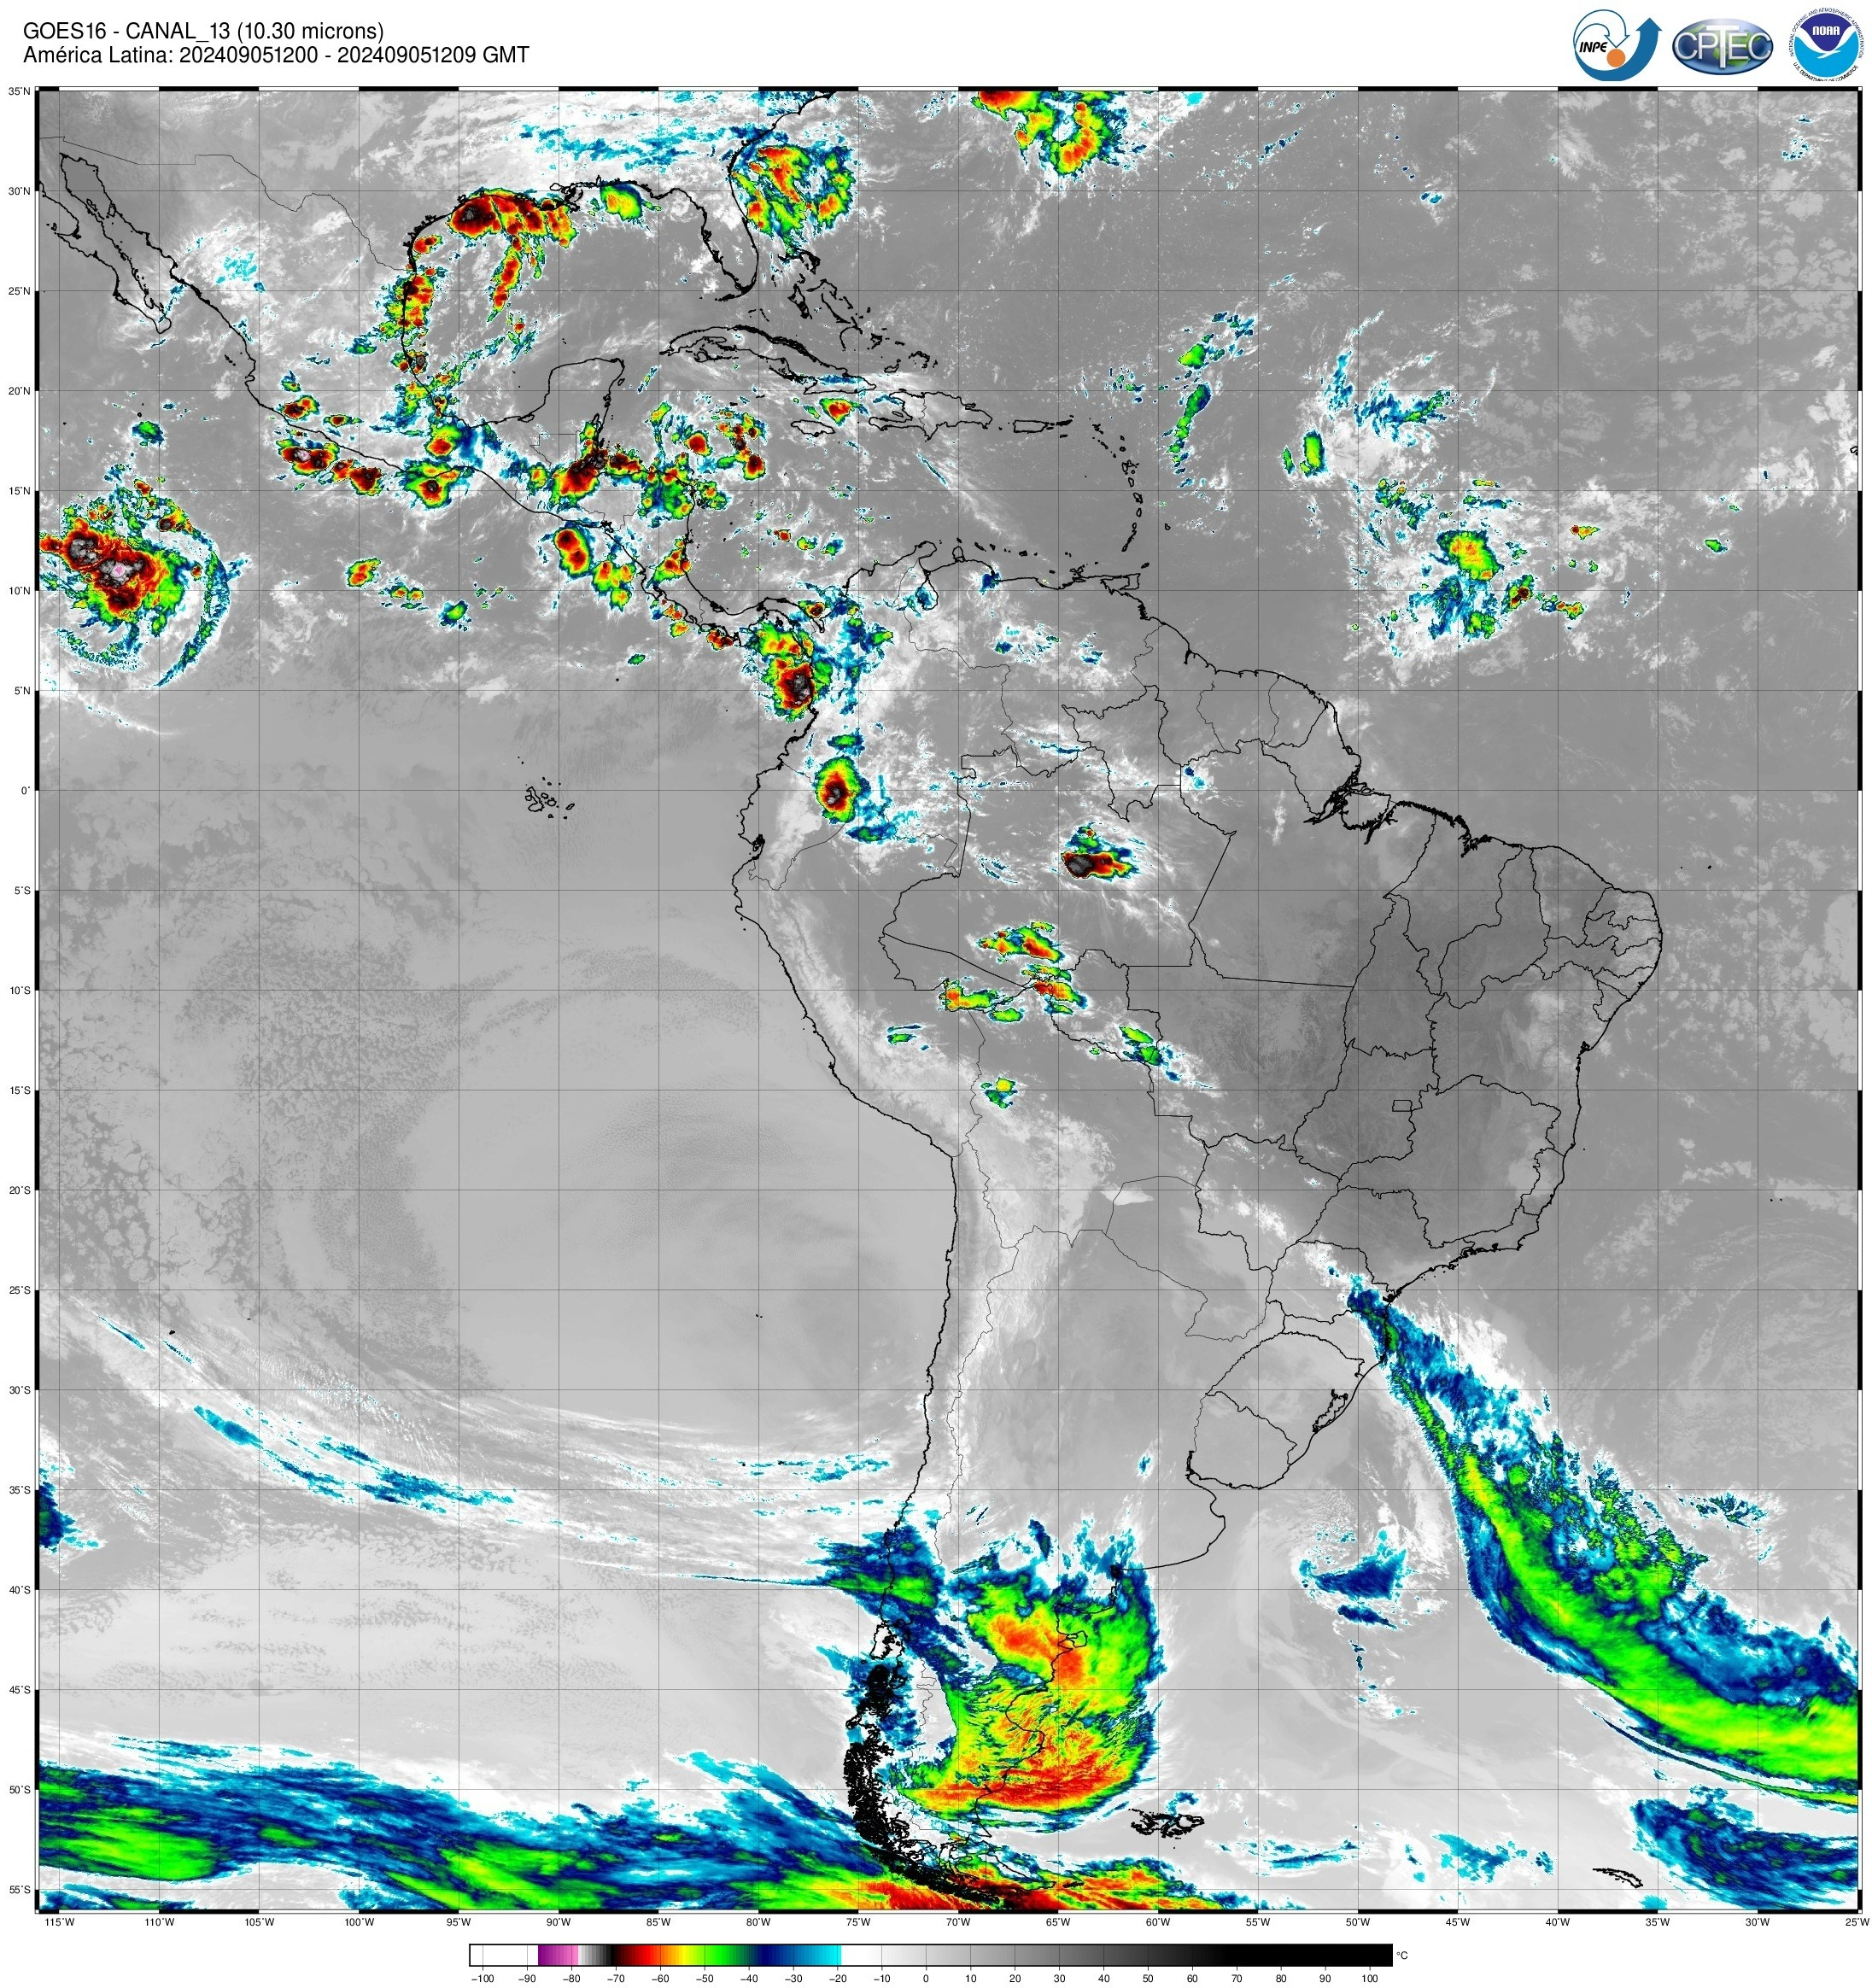
\includegraphics[width=\textwidth, trim=0cm 0cm 0cm 3.5cm, clip]{images/goes16_ch13_202409051200.jpg}
	\caption{2024-09-05T12:00}
	\label{fig:goes16_ch13_202409051200}
	\end{subfigure}
	\hfill
	\begin{subfigure}[b]{0.4\textwidth}
		\centering
		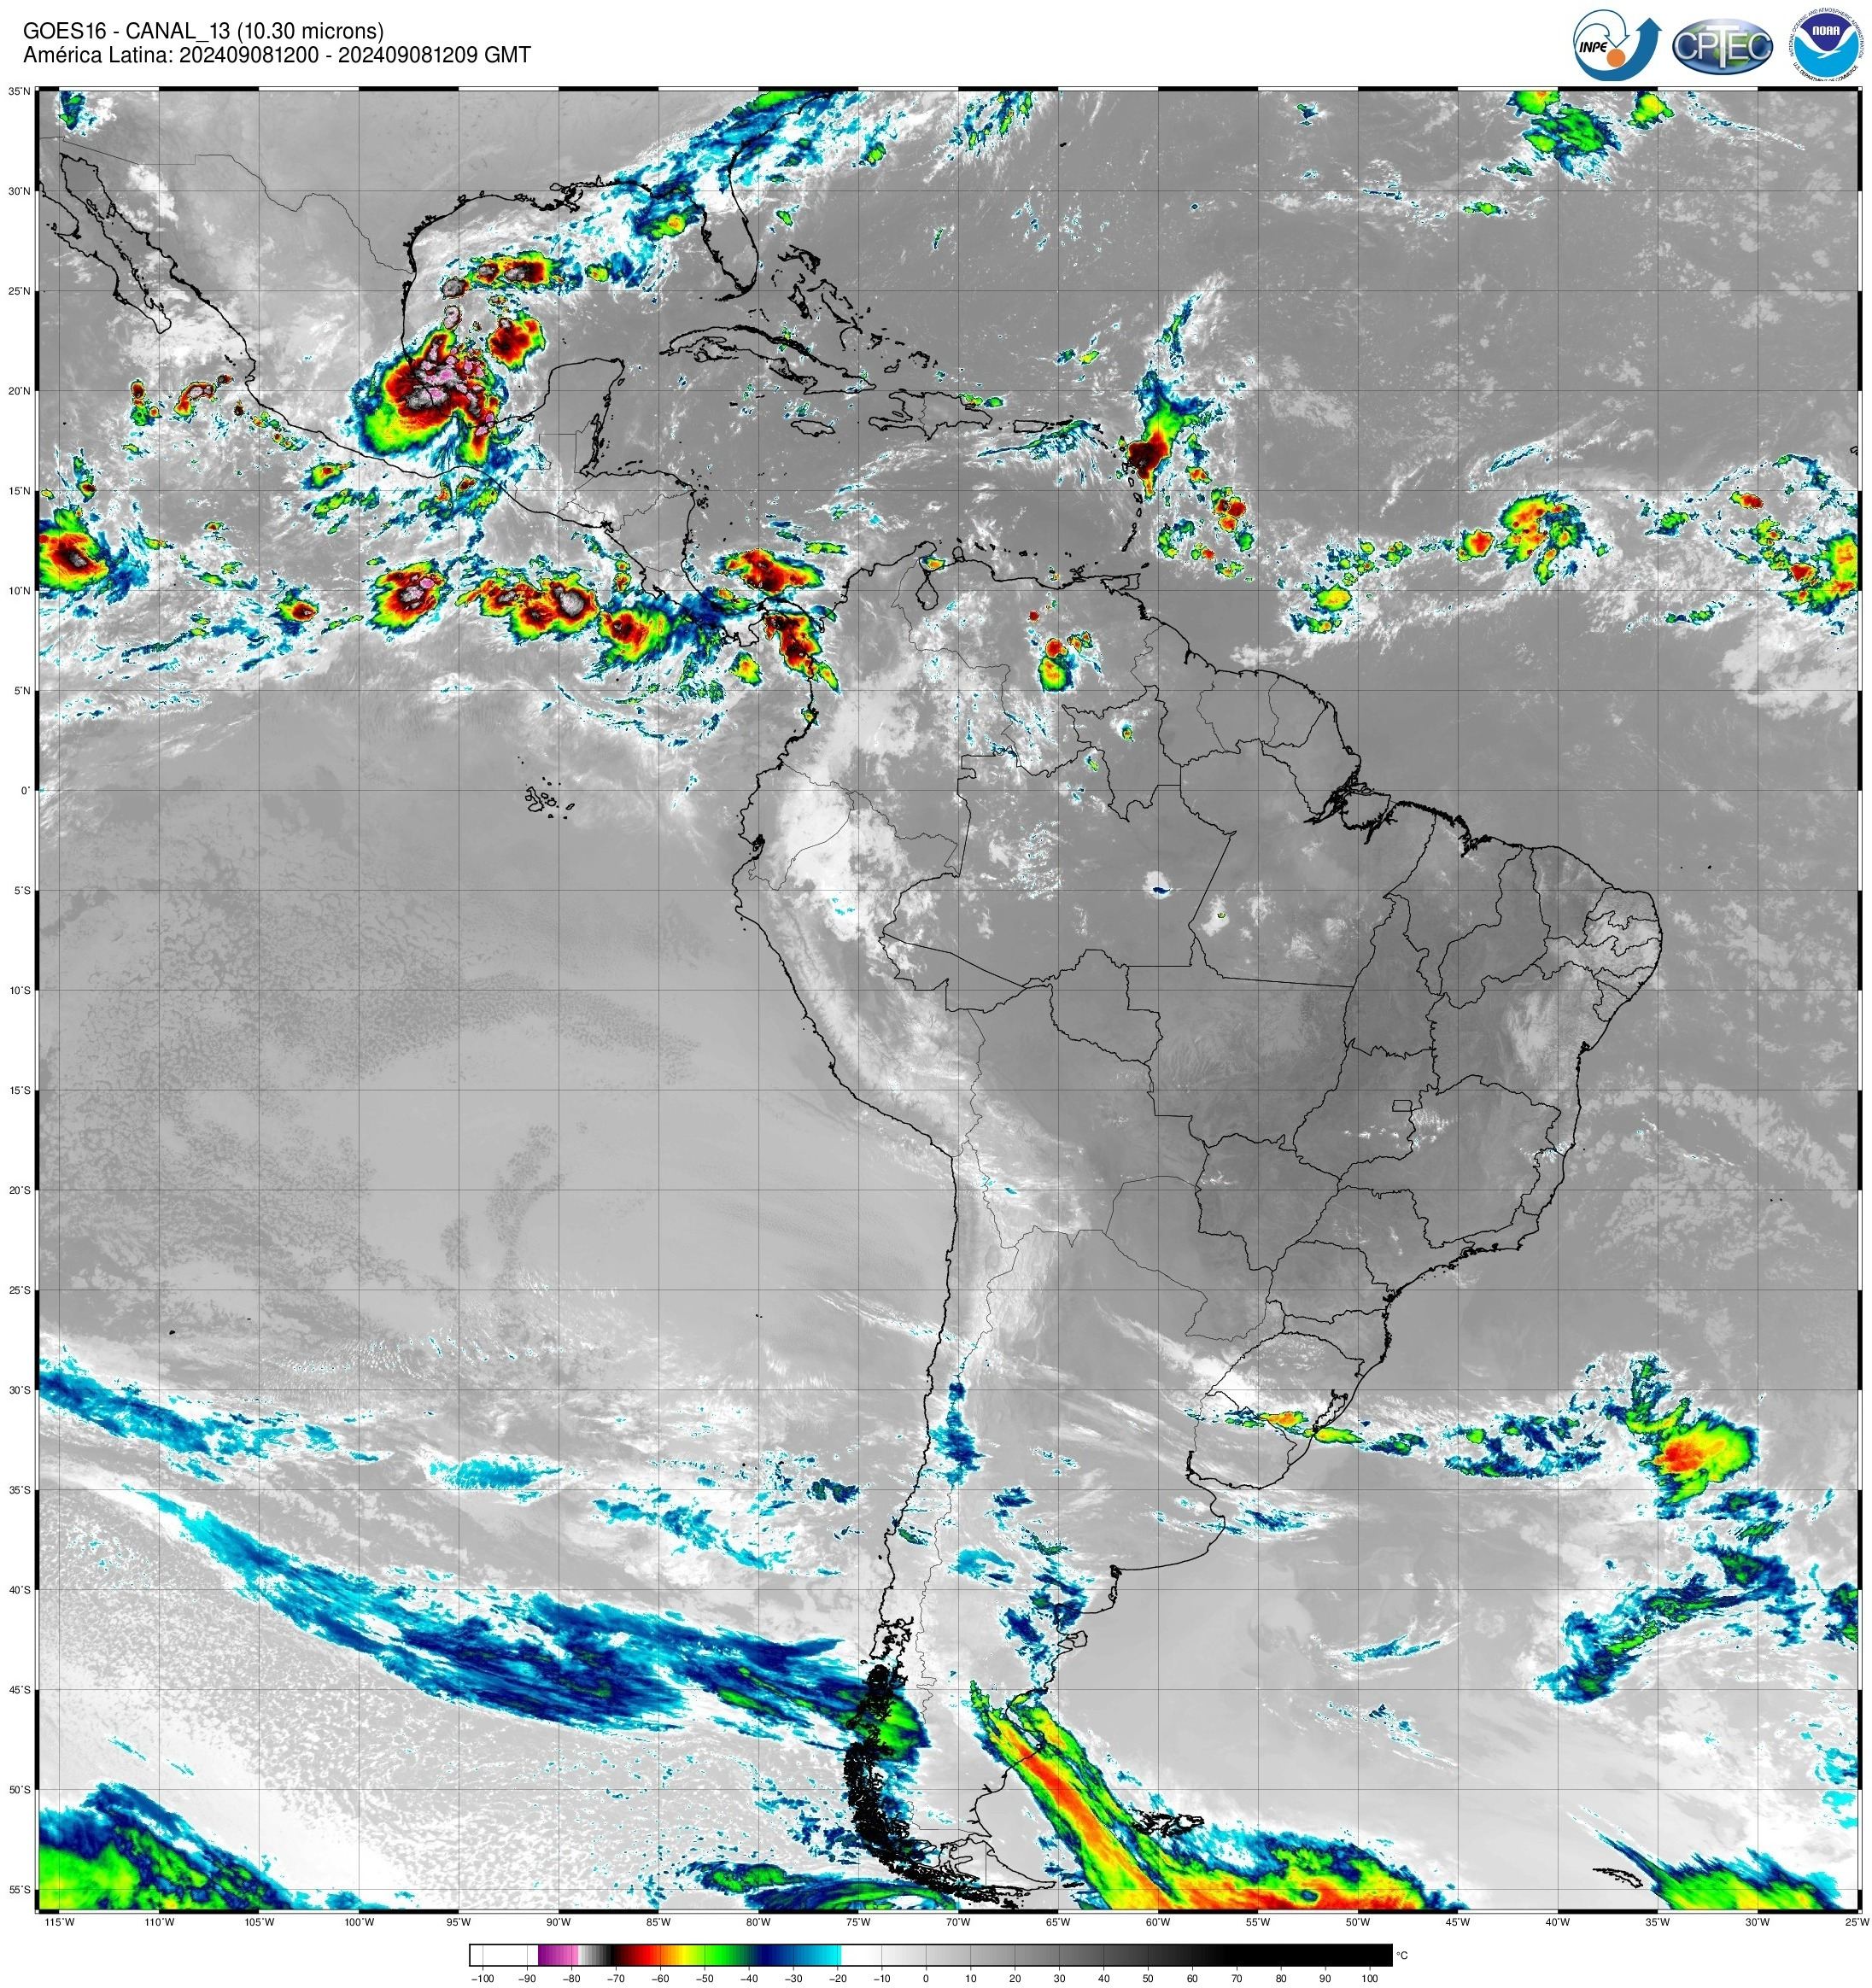
\includegraphics[width=\textwidth, trim=0cm 0cm 0cm 3.5cm, clip]{images/goes16_ch13_202409081200.jpg}
		\caption{2024-09-08T12:00}
		\label{fig:goes16_ch13_202409081200}
	\end{subfigure}
	\hfill
	\begin{subfigure}[b]{0.4\textwidth}
		\centering
		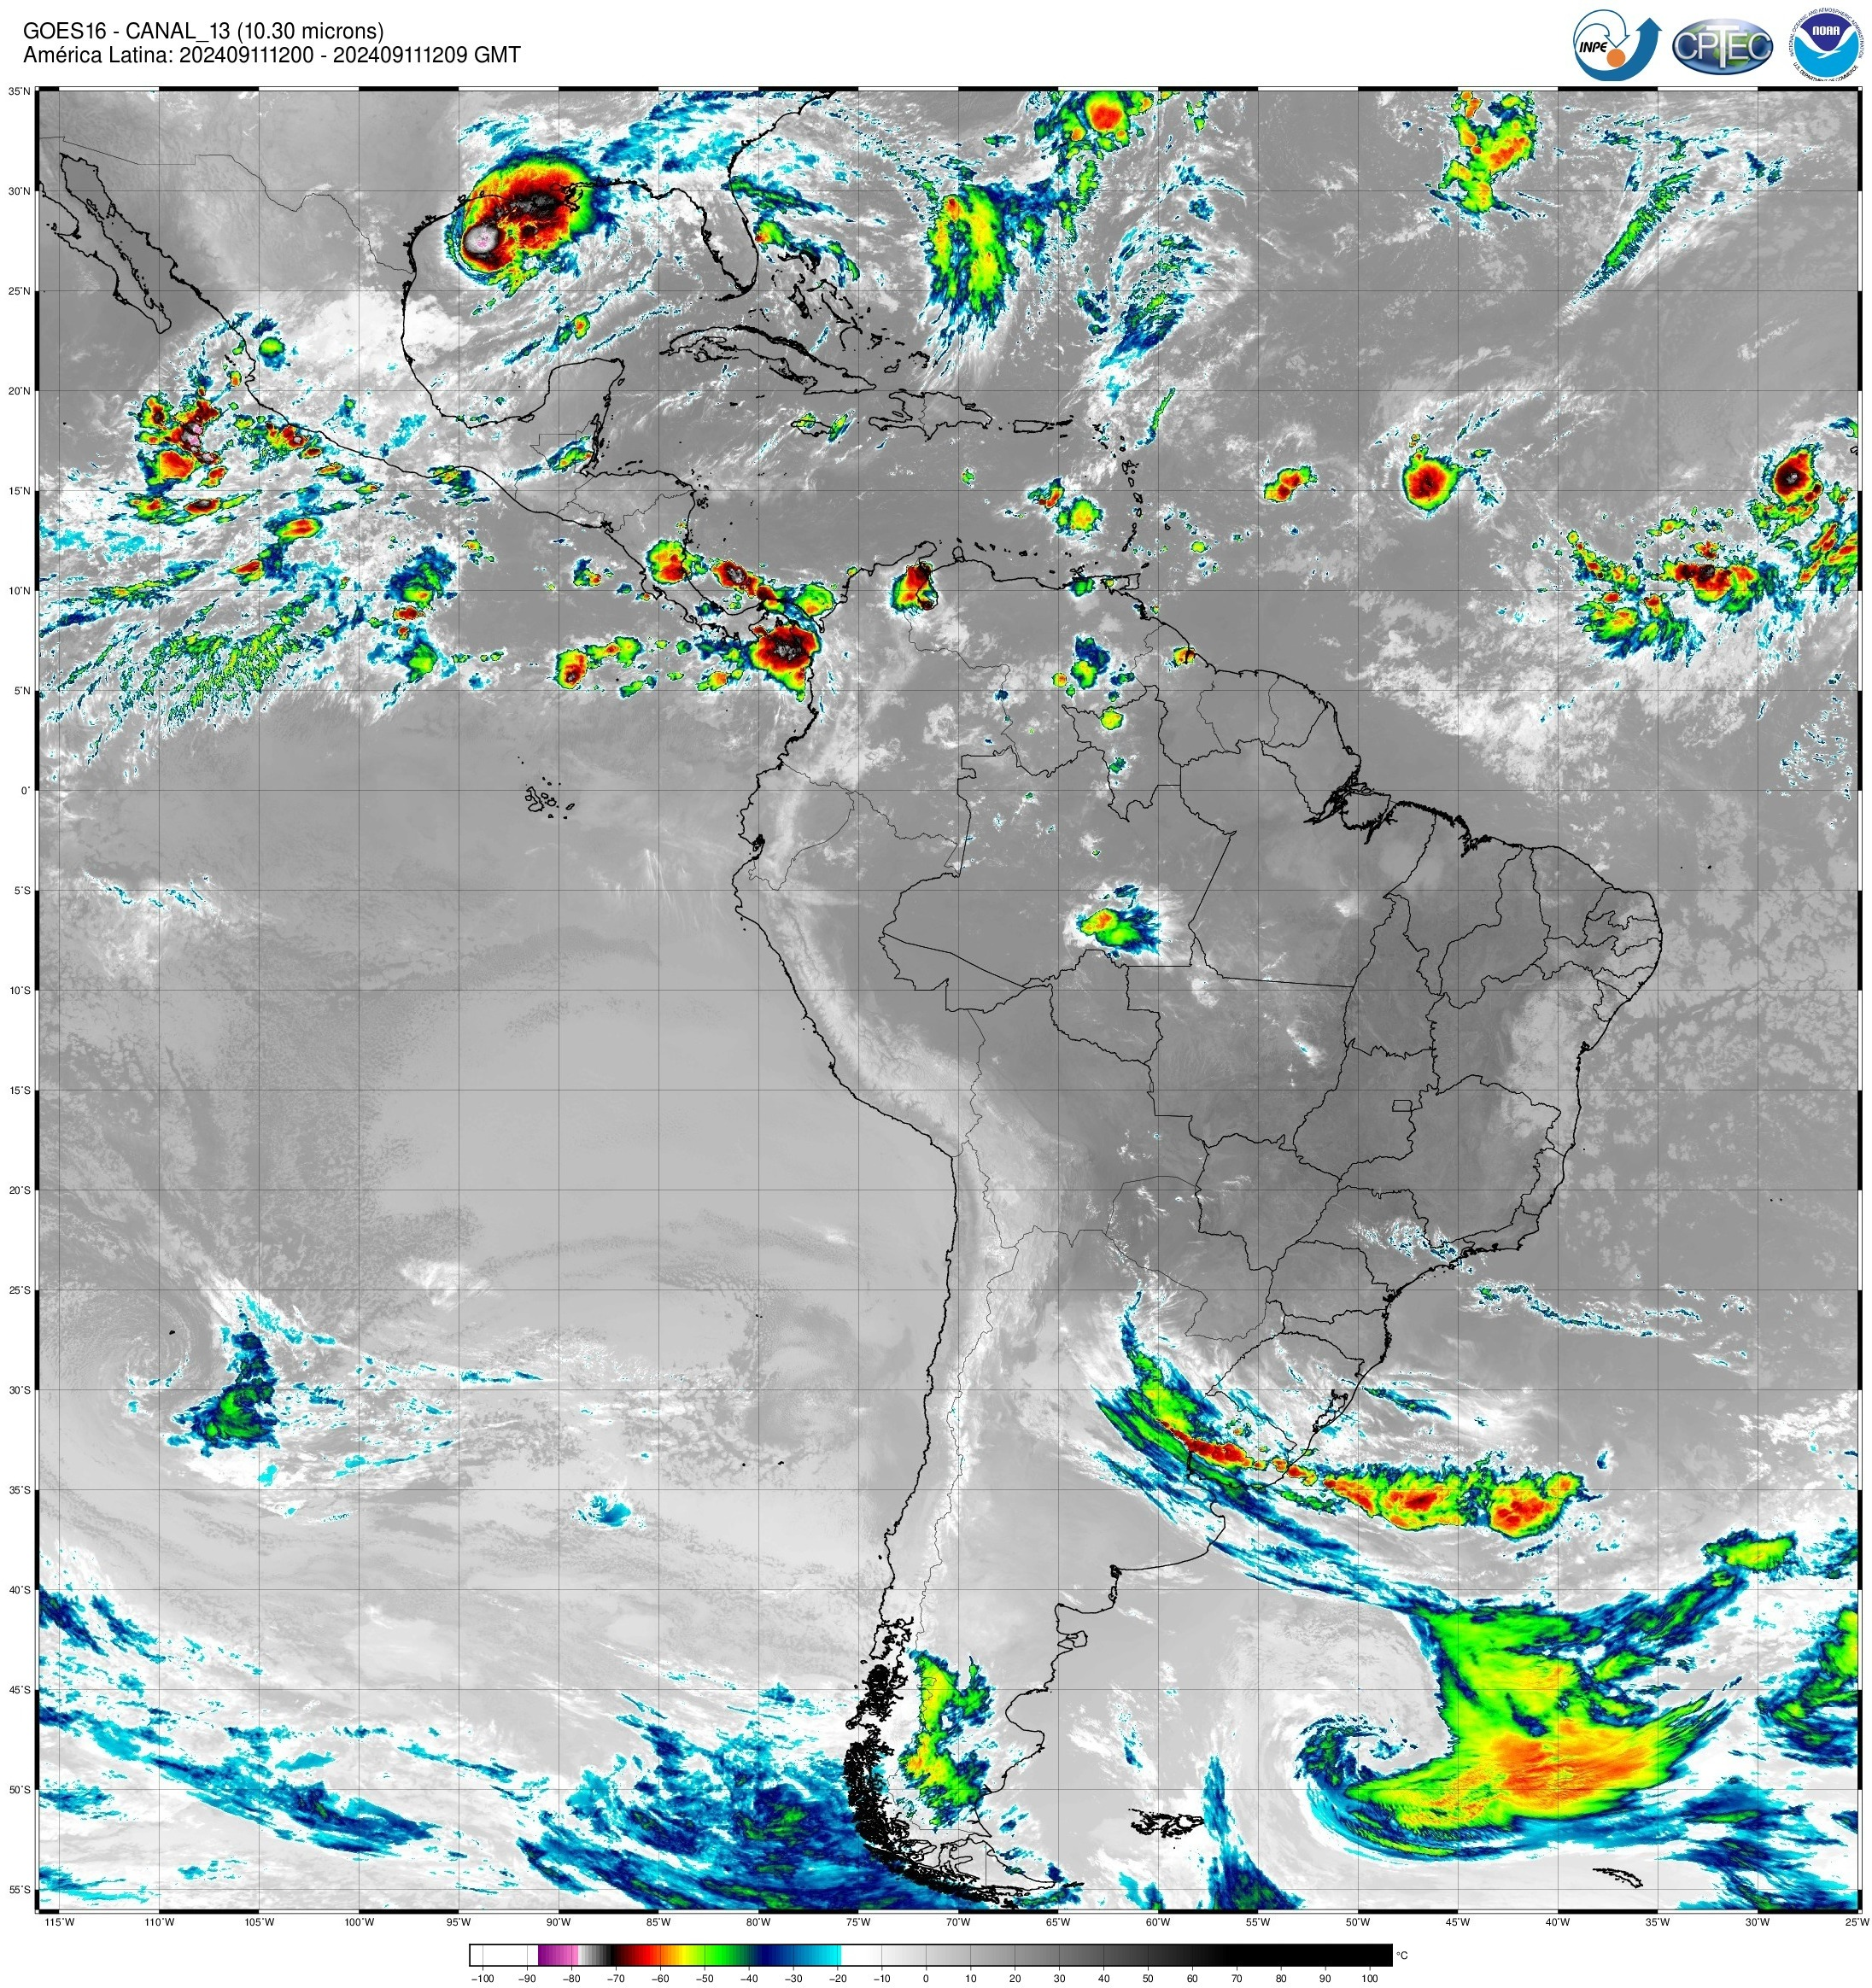
\includegraphics[width=\textwidth, trim=0cm 0cm 0cm 3.5cm, clip]{images/goes16_ch13_202409111200.jpg}
		\caption{2024-09-11T12:00}
		\label{fig:goes16_ch13_202409111200}
	\end{subfigure}
	\hfill
	\begin{subfigure}[b]{0.4\textwidth}
		\centering
		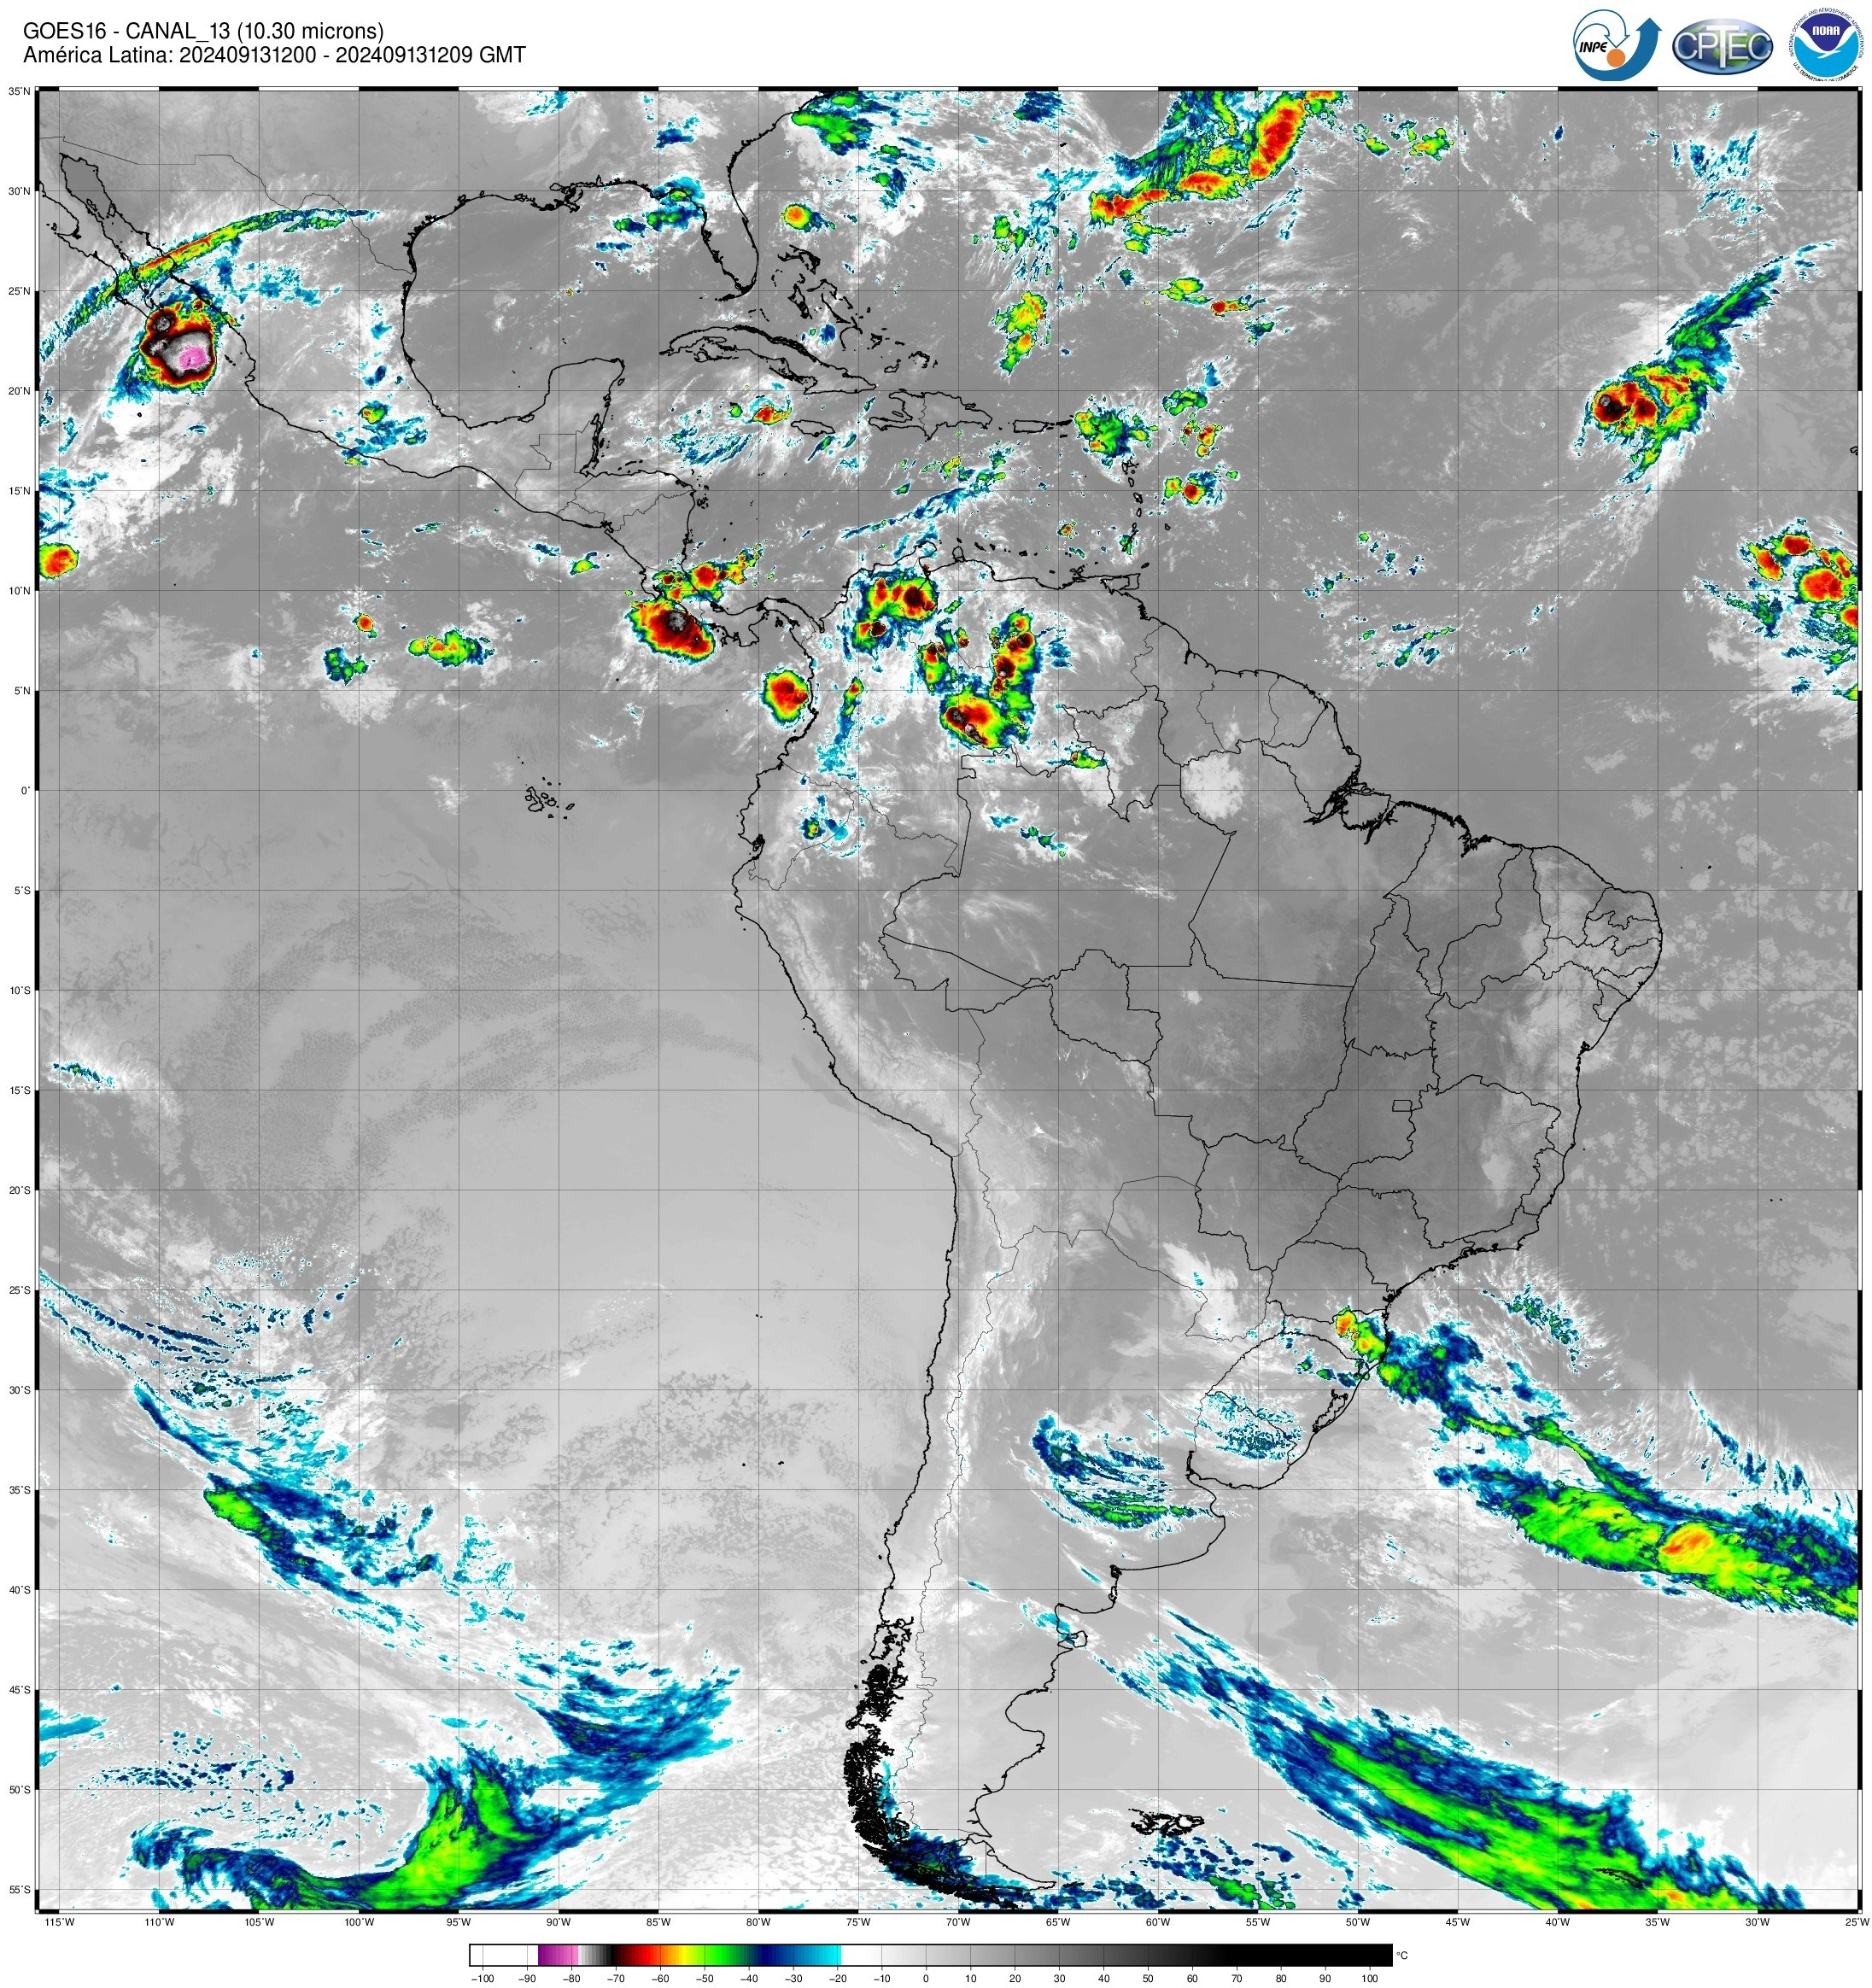
\includegraphics[width=\textwidth, trim=0cm 0cm 0cm 3.5cm, clip]{images/goes16_ch13_202409131200.jpg}
		\caption{2024-09-13T12:00}
		\label{fig:goes16_ch13_202409131200}
	\end{subfigure}
	\caption{Imagens do satélite GOES16 no canal 13 para entre os dias 05 e 13 de setembro de 2024}
	\label{fig:goesgeral}	
\end{figure}




Com o objetivo de analisar as condições da circulação atmosférica que podem ter contribuído para o aumento da concentração de aerossóis, como o black carbon (BC), sobre Santa Catarina, foram analisados os campos de vento em 750, 800 e 850 hPa para os dias 11, 12 e 13 de setembro, conforme apresentado na Figura 8. Os resultados evidenciam um padrão de circulação atmosférica associado ao South American Low-Level Jet (SALLJ), com escoamento direcionado para a região Sul do Brasil, em concordância com as análises preliminares apresentadas por \autocite{forgioni2025}.
Esses resultados sugerem que a circulação atmosférica favoreceu o transporte de aerossóis para Santa Catarina, contribuindo para o aumento dos valores de AOD observados no estado, especialmente na região Oeste, que constitui a primeira área do estado impactada pelo transporte dessas partículas. 




\begin{figure}[htbp]
	\centering
	% --- LINHA 1 ---
	\begin{subfigure}[b]{0.31\textwidth}
		\centering
		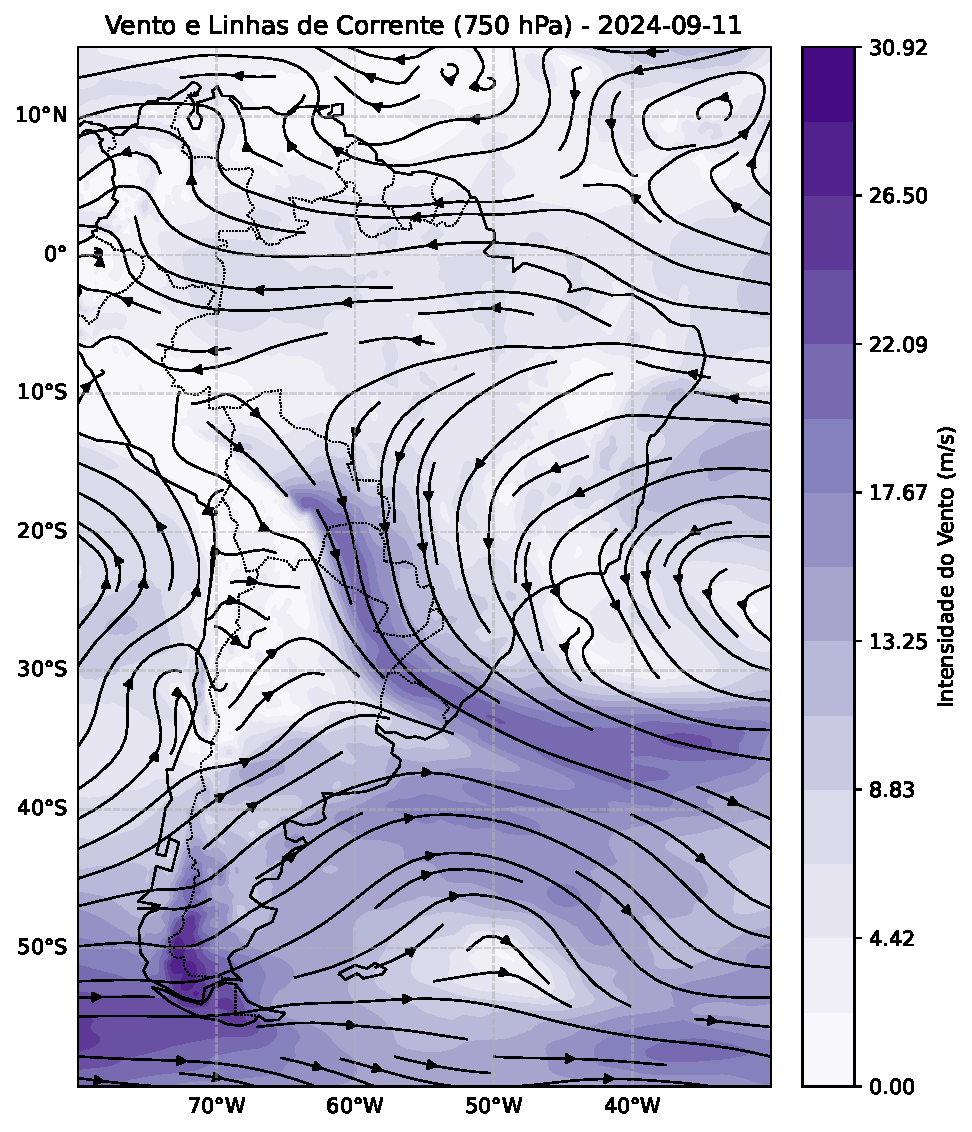
\includegraphics[width=\textwidth, trim=0cm 0cm 0cm 0.6cm, clip]{images/vento_750hPa_2024-09-11.pdf}
		\caption{750hPa 2024-09-11}
		\label{fig:img1}
	\end{subfigure}
	\hfill
	\begin{subfigure}[b]{0.31\textwidth}
		\centering
		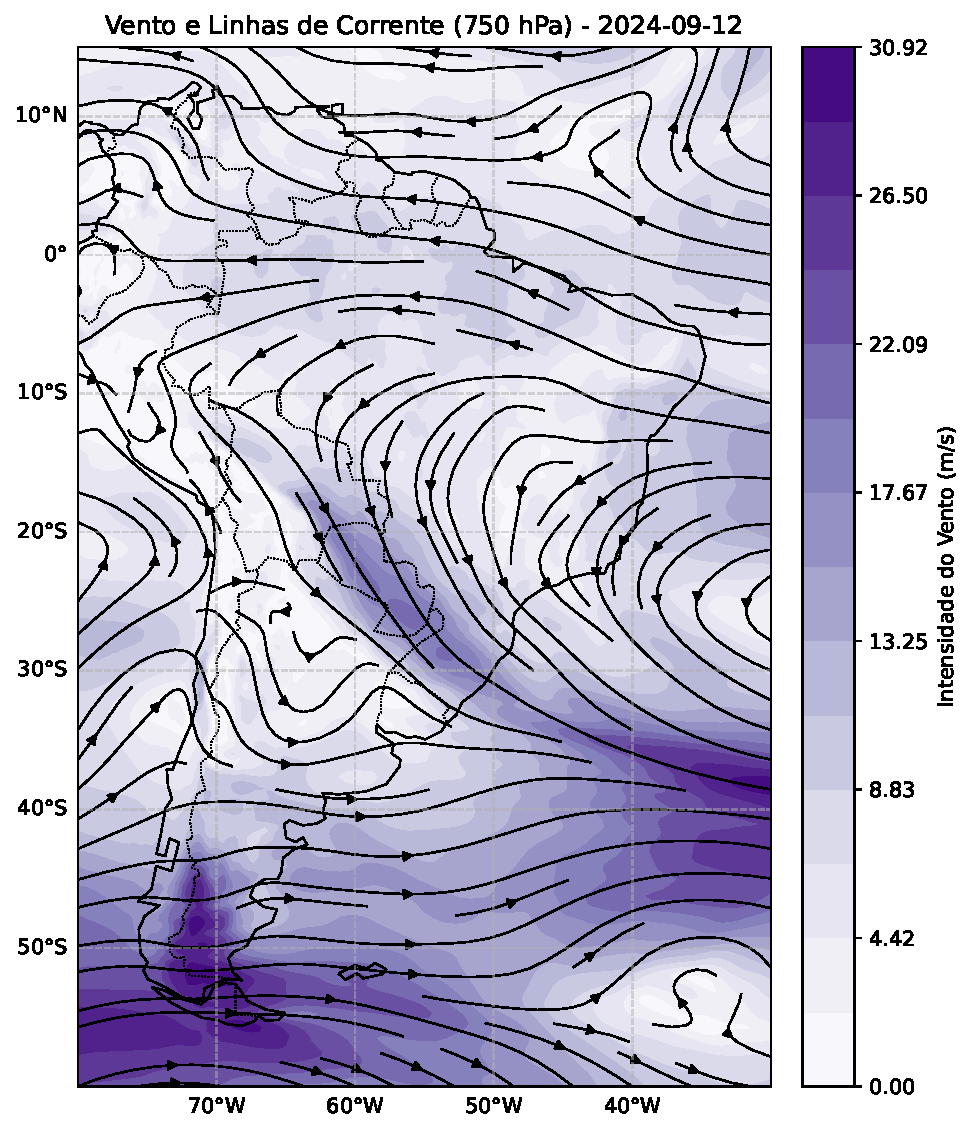
\includegraphics[width=\textwidth, trim=0cm 0cm 0cm 0.6cm, clip]{images/vento_750hPa_2024-09-12.pdf}
		\caption{750hPa 2024-09-12}
		\label{fig:img2}
	\end{subfigure}
	\hfill
	\begin{subfigure}[b]{0.31\textwidth}
		\centering
		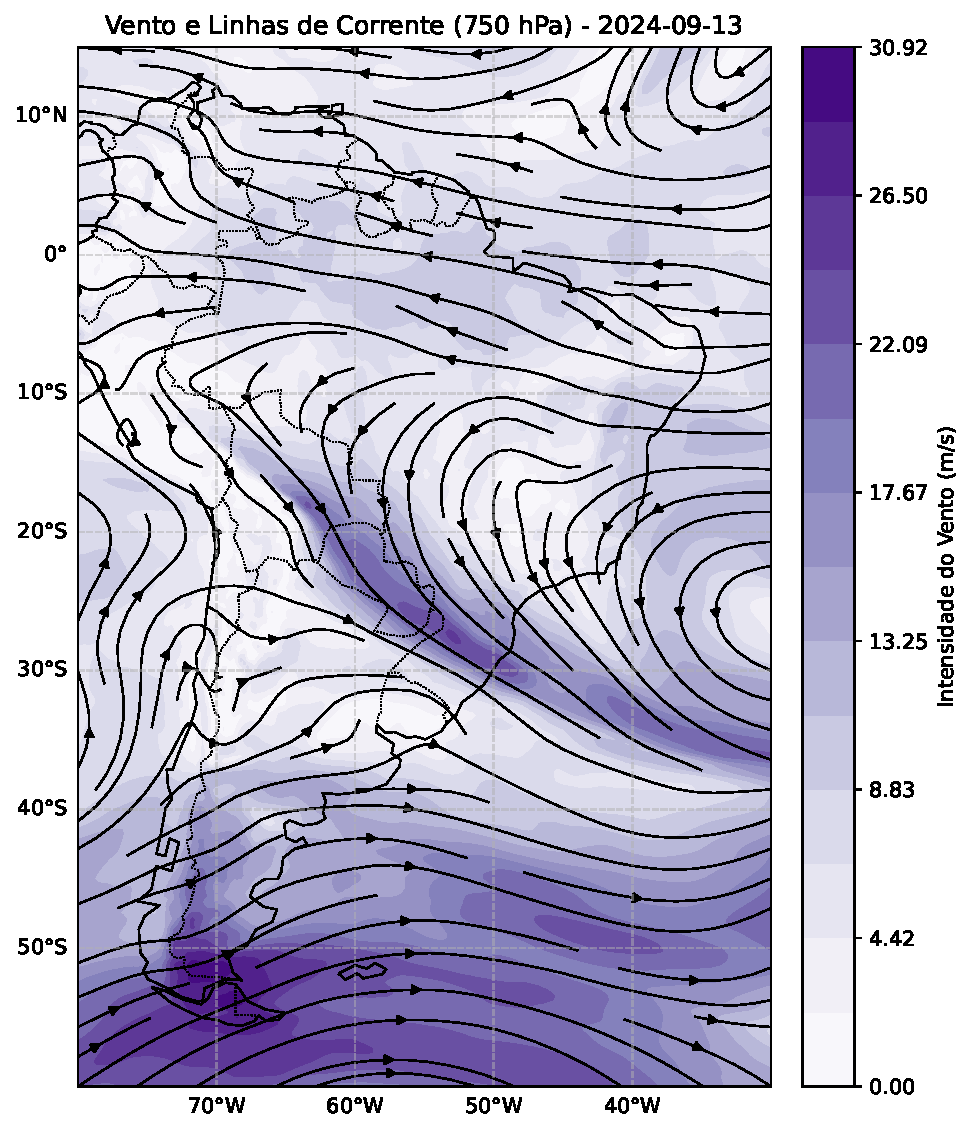
\includegraphics[width=\textwidth, trim=0cm 0cm 0cm 0.6cm, clip]{images/vento_750hPa_2024-09-13.pdf}
		\caption{750hPa 2024-09-13}
		\label{fig:img3}
	\end{subfigure}
	
	\vspace{0.8em} % Espaçamento vertical entre as linhas
	
	% --- LINHA 2 ---
	\begin{subfigure}[b]{0.31\textwidth}
		\centering
		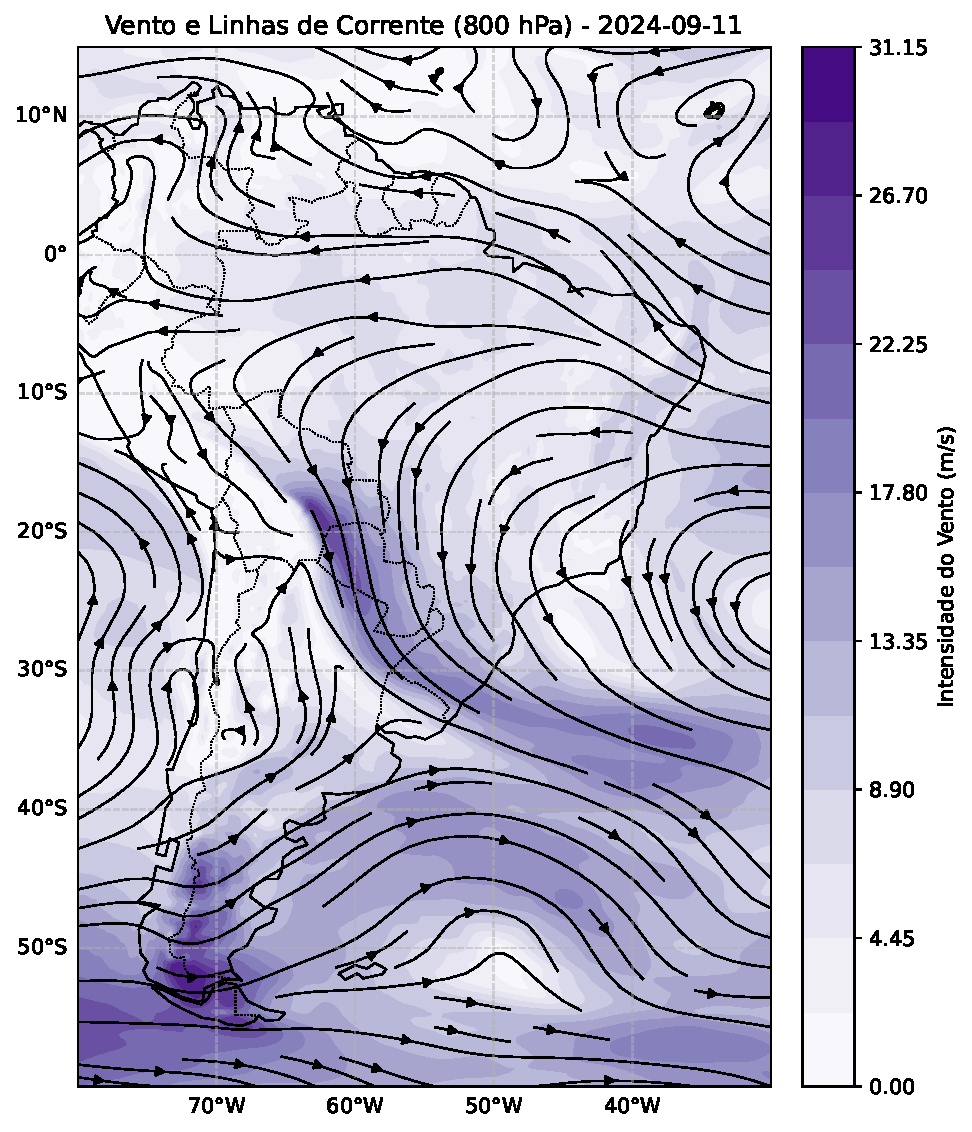
\includegraphics[width=\textwidth, trim=0cm 0cm 0cm 0.6cm, clip]{images/vento_800hPa_2024-09-11.pdf}
		\caption{800hPa 2024-09-11}
		\label{fig:img4}
	\end{subfigure}
	\hfill
	\begin{subfigure}[b]{0.31\textwidth}
		\centering
		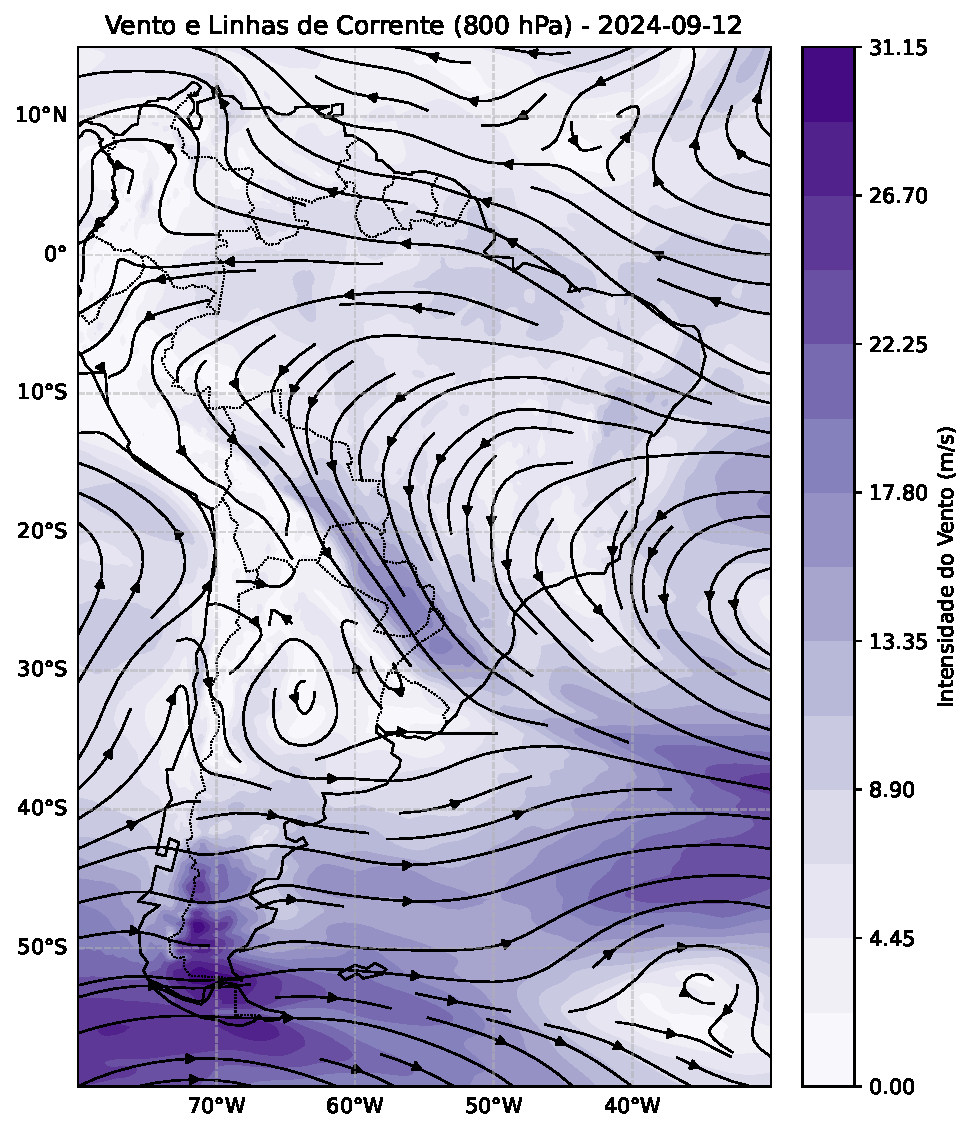
\includegraphics[width=\textwidth, trim=0cm 0cm 0cm 0.6cm, clip]{images/vento_800hPa_2024-09-12.pdf}
		\caption{800hPa 2024-09-12}
		\label{fig:img5}
	\end{subfigure}
	\hfill
	\begin{subfigure}[b]{0.31\textwidth}
		\centering
		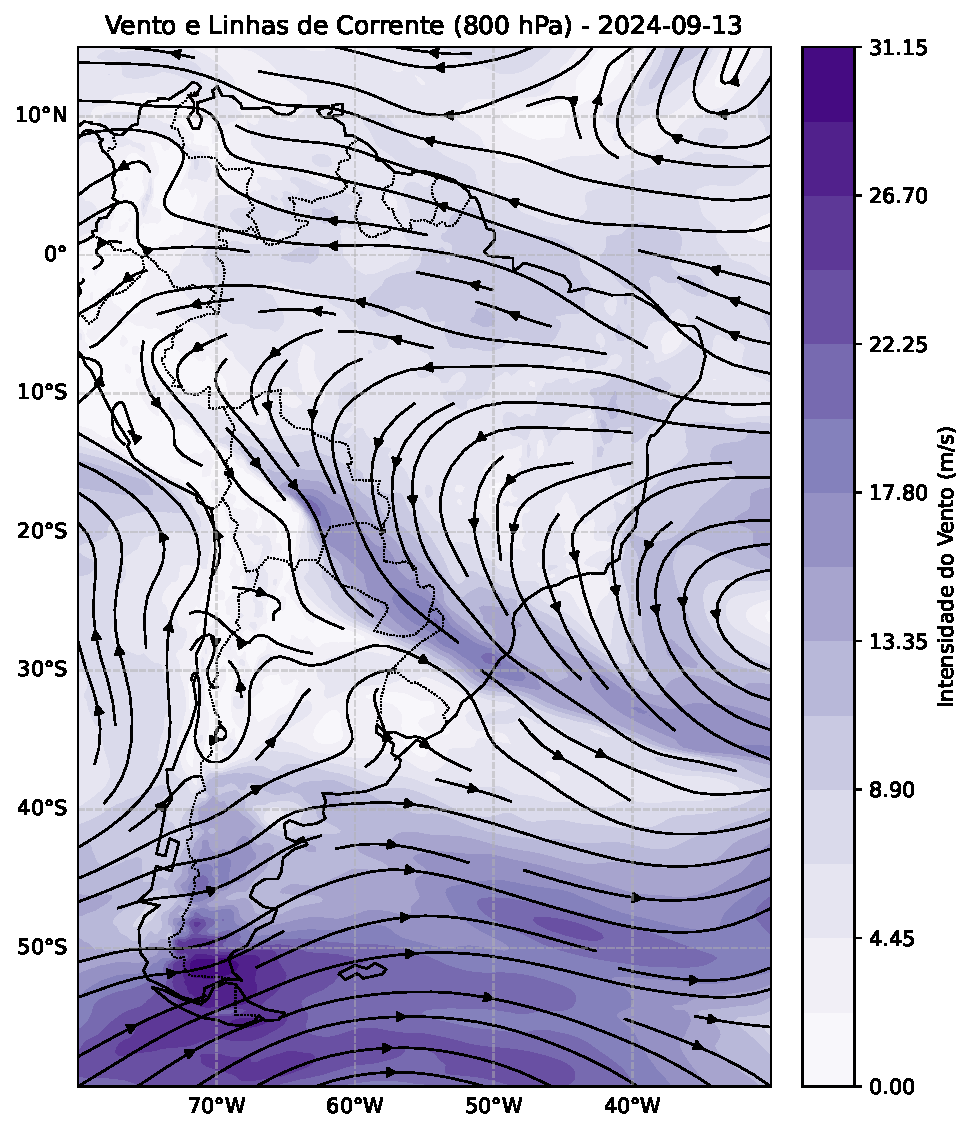
\includegraphics[width=\textwidth, trim=0cm 0cm 0cm 0.6cm, clip]{images/vento_800hPa_2024-09-13.pdf}
		\caption{800hPa 2024-09-13}
		\label{fig:img6}
	\end{subfigure}
	
	\vspace{0.8em} % Espaçamento vertical entre as linhas
	
	% --- LINHA 3 ---
	\begin{subfigure}[b]{0.31\textwidth}
		\centering
		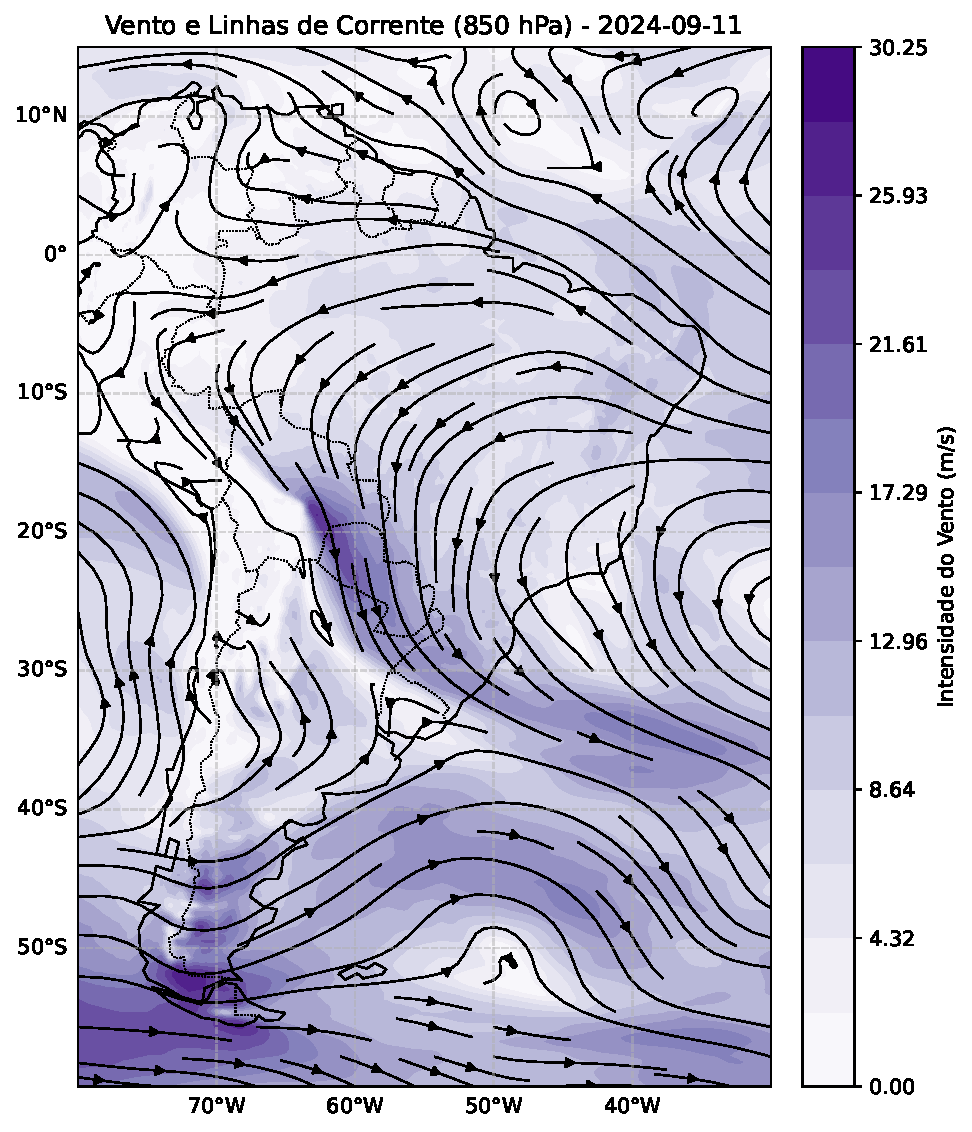
\includegraphics[width=\textwidth, trim=0cm 0cm 0cm 0.6cm, clip]{images/vento_850hPa_2024-09-11.pdf}
		\caption{850hPa 2024-09-11}
		\label{fig:img7}
	\end{subfigure}
	\hfill
	\begin{subfigure}[b]{0.31\textwidth}
		\centering
		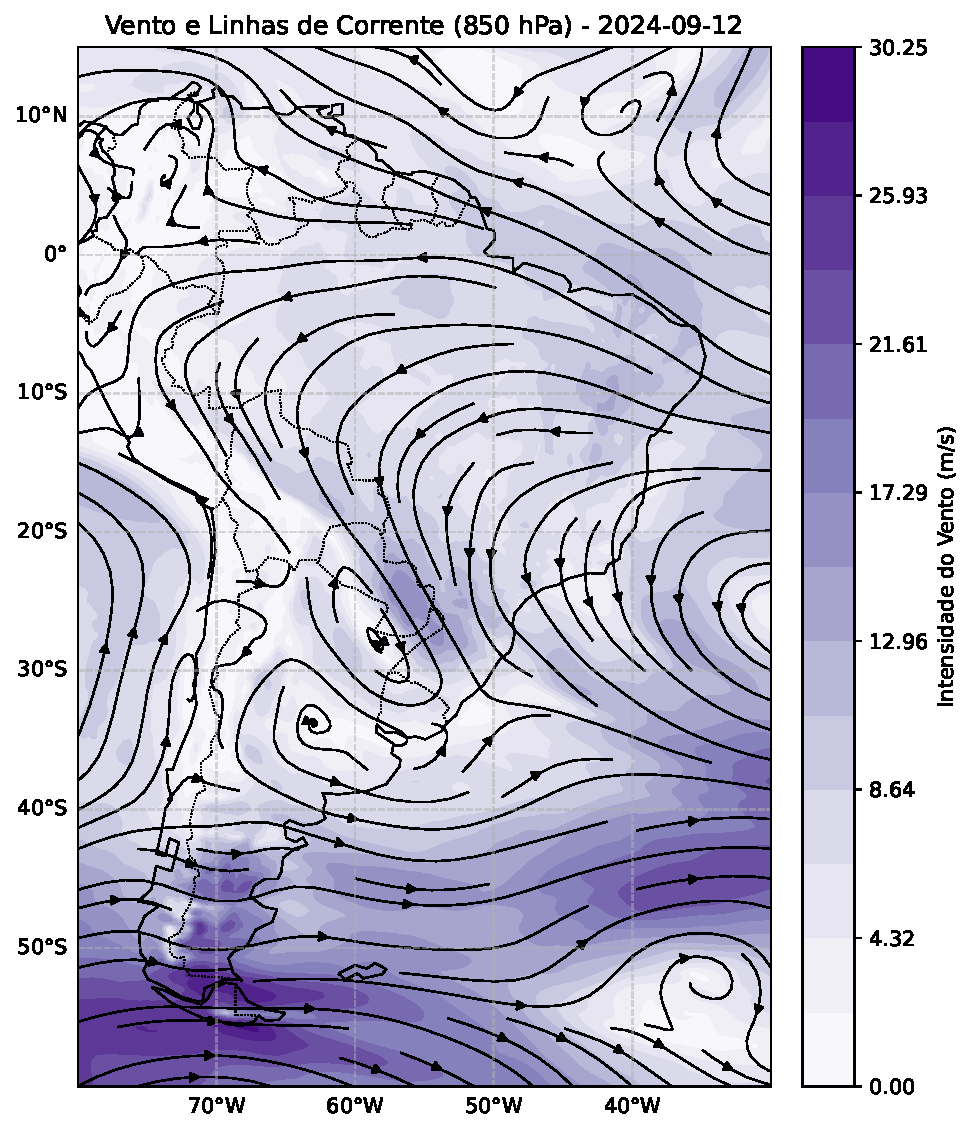
\includegraphics[width=\textwidth,
		trim=0cm 0cm 0cm 0.6cm, clip]{images/vento_850hPa_2024-09-12.pdf}
		\caption{850hPa 2024-09-12}
		\label{fig:img8}
	\end{subfigure}
	\hfill
	\begin{subfigure}[b]{0.31\textwidth}
		\centering
		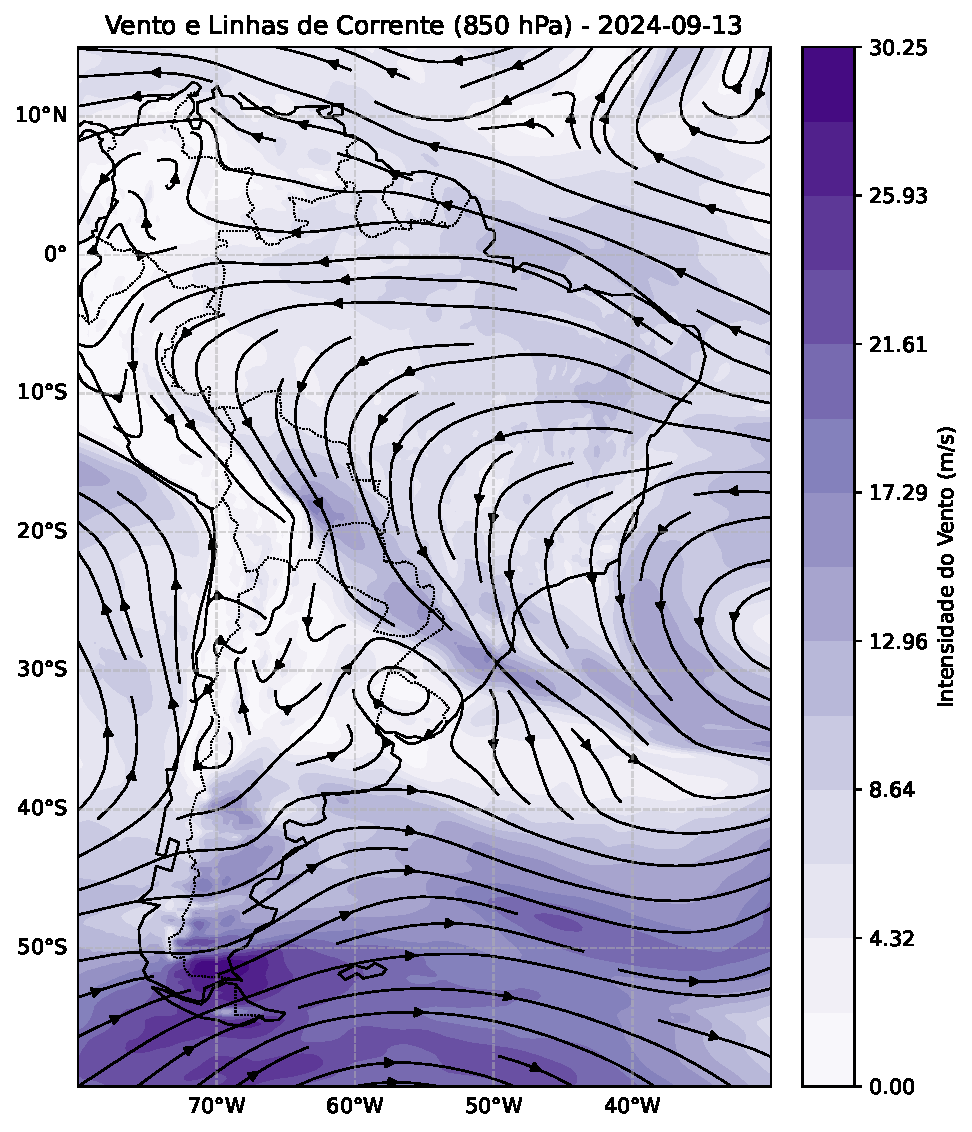
\includegraphics[width=\textwidth, trim=0cm 0cm 0cm 0.6cm, clip]{images/vento_850hPa_2024-09-13.pdf}
		\caption{850hPa 2024-09-13}
		\label{fig:img9}
	\end{subfigure}
	
	\caption{Médias diárias de direção e intensidade do vento.}
	\label{fig:grade_completa}
\end{figure}


\begin{figure}[htbp]
	\centering
	% --- LINHA 1 ---
	\begin{subfigure}[b]{0.31\textwidth}
		\centering
		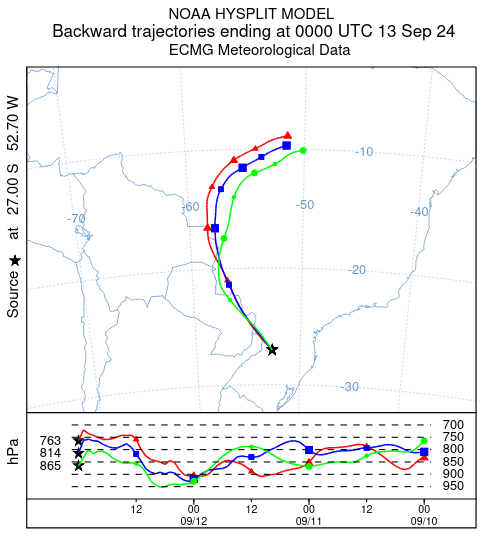
\includegraphics[width=\textwidth, trim=0cm 0cm 0cm 2.1cm, clip]{images/chapeco_traj.png}
		\caption{Chapecó, SC}
		\label{fig:img42}
	\end{subfigure}
	\hfill
	\begin{subfigure}[b]{0.31\textwidth}
		\centering
		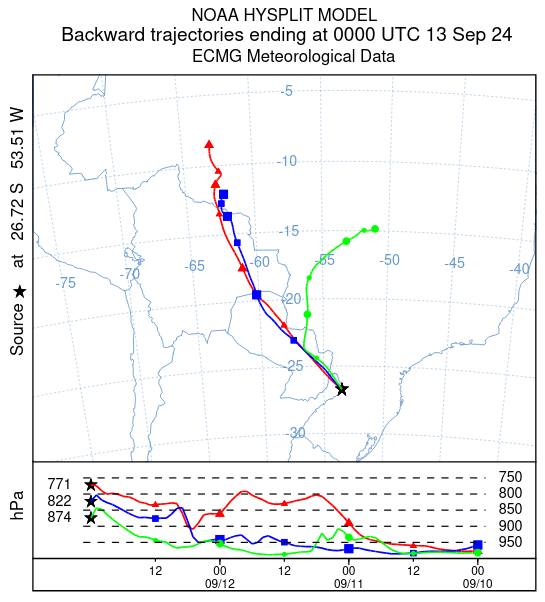
\includegraphics[width=\textwidth, trim=0cm 0cm 0cm 2.3cm, clip]{images/saomiguel_traj.png}
		\caption{São Miguel do Oeste, SC}
		\label{fig:img43}
	\end{subfigure}
	\hfill
	\begin{subfigure}[b]{0.31\textwidth}
		\centering
		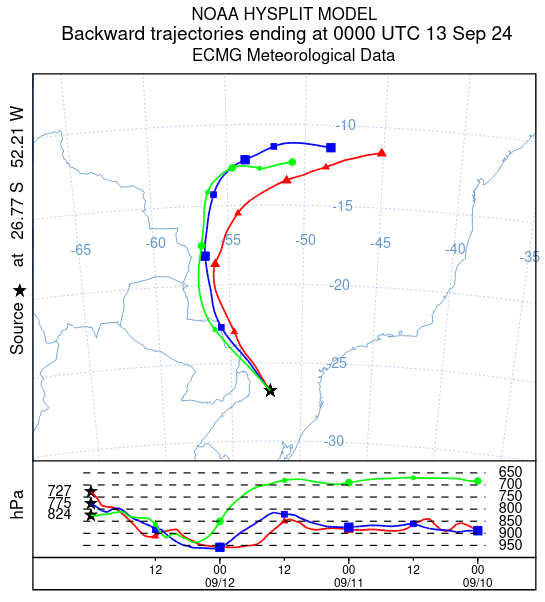
\includegraphics[width=\textwidth, trim=0cm 0cm 0cm 2.3cm, clip]{images/maravilha_traj.png}
		\caption{Maravilha, SC}
		\label{fig:img44}
	\end{subfigure}
	\caption{Trajetórias reversas nos níveis de 750, 800 e 850 hPa entre os dias 09 e 13 de setembro de 2024.}
	\label{fig:traj}
\end{figure}


\begin{figure}[htbp]
	\centering
	% --- LINHA 1 ---
	\begin{subfigure}[b]{0.31\textwidth}
		\centering
		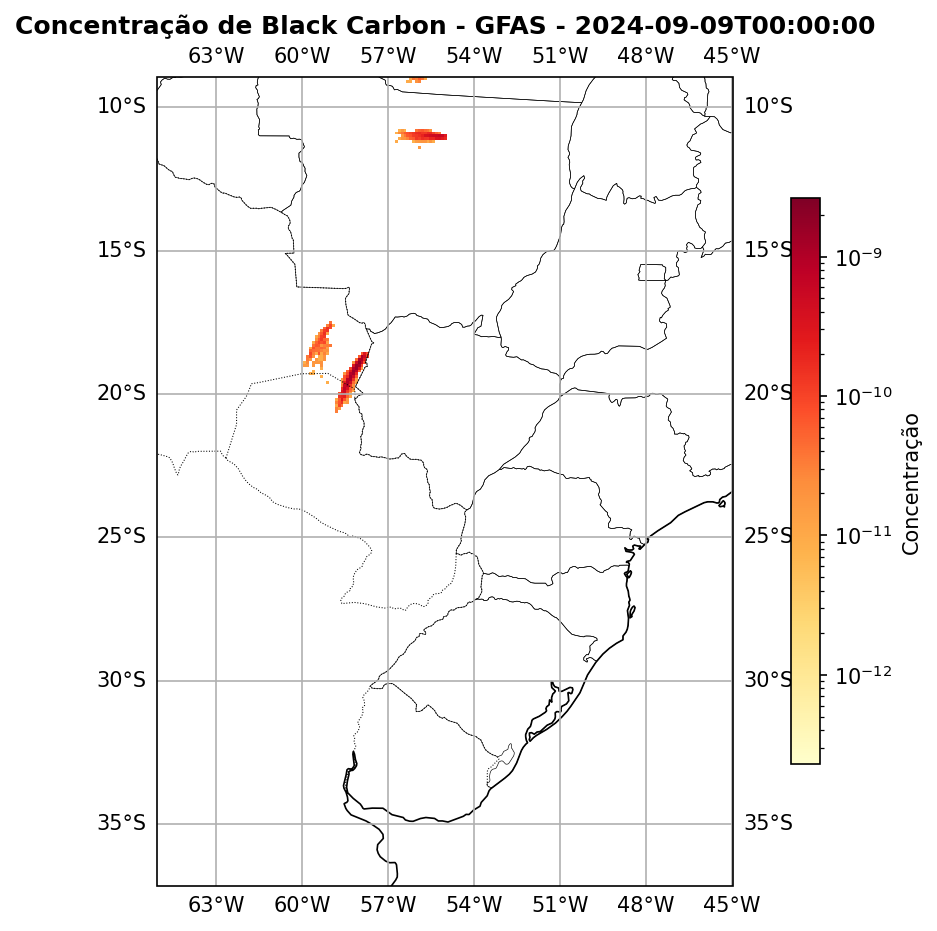
\includegraphics[width=\textwidth, trim=0cm 0cm 0cm 0.7cm, clip]{images/bc_000.png}
		\caption{2024-09-09 00:00:00}
		\label{fig:img10}
	\end{subfigure}
	\hfill
	\begin{subfigure}[b]{0.31\textwidth}
		\centering
		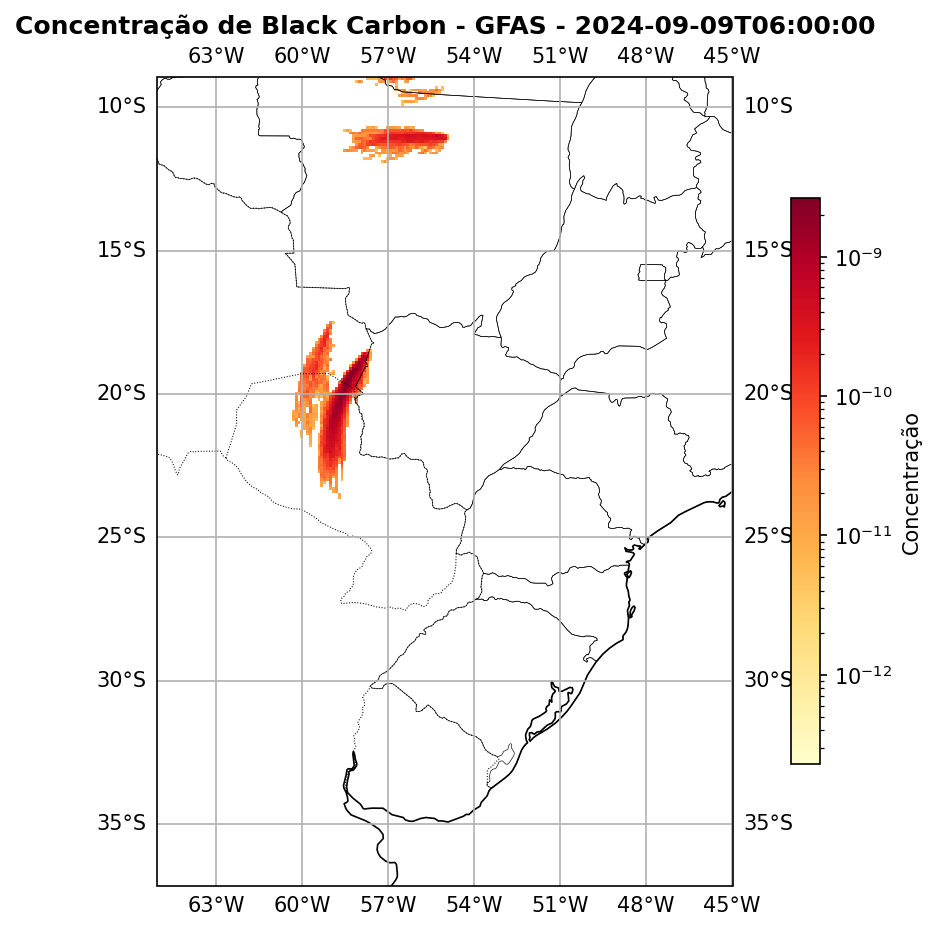
\includegraphics[width=\textwidth, trim=0cm 0cm 0cm 0.7cm, clip]{images/bc_001.png}
		\caption{2024-09-09 00:06:00}
		\label{fig:img11}
	\end{subfigure}
	\hfill
	\begin{subfigure}[b]{0.31\textwidth}
		\centering
		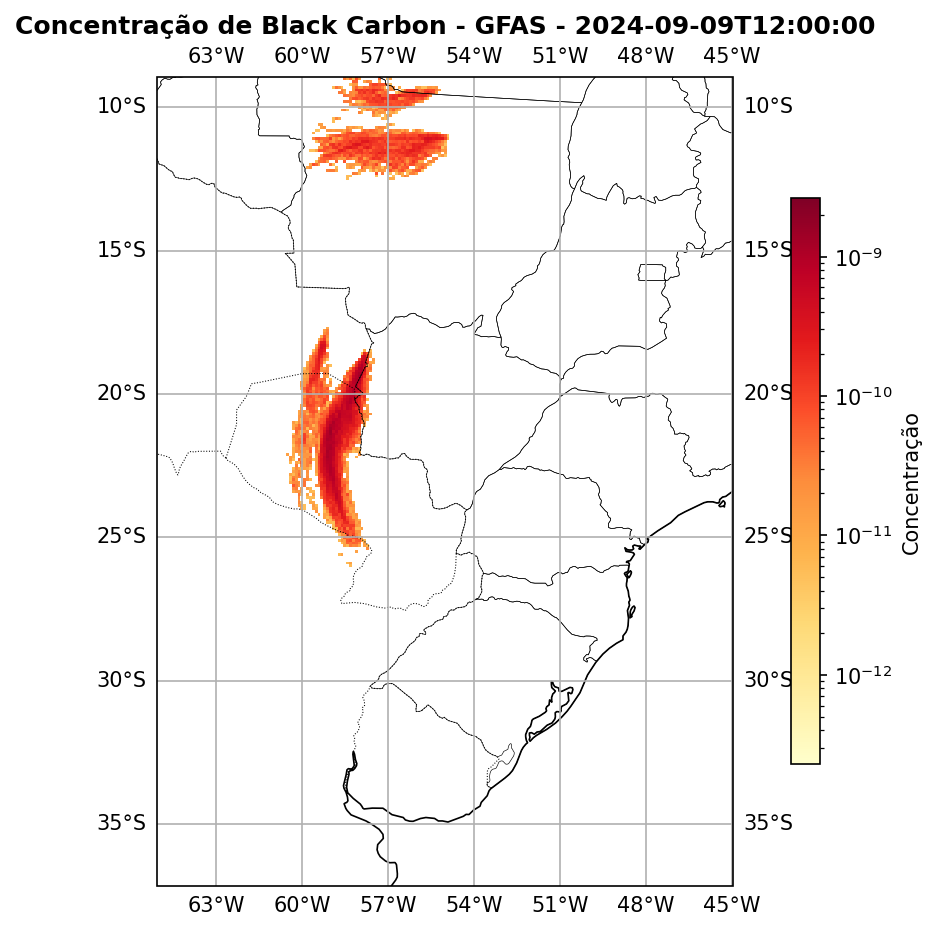
\includegraphics[width=\textwidth, trim=0cm 0cm 0cm 0.7cm, clip]{images/bc_002.png}
		\caption{2024-09-09 00:12:00}
		\label{fig:img12}
	\end{subfigure}
	\hfill
	
	\vspace{0.8em} % Espaçamento vertical entre as linhas
	
	\begin{subfigure}[b]{0.31\textwidth}
		\centering
		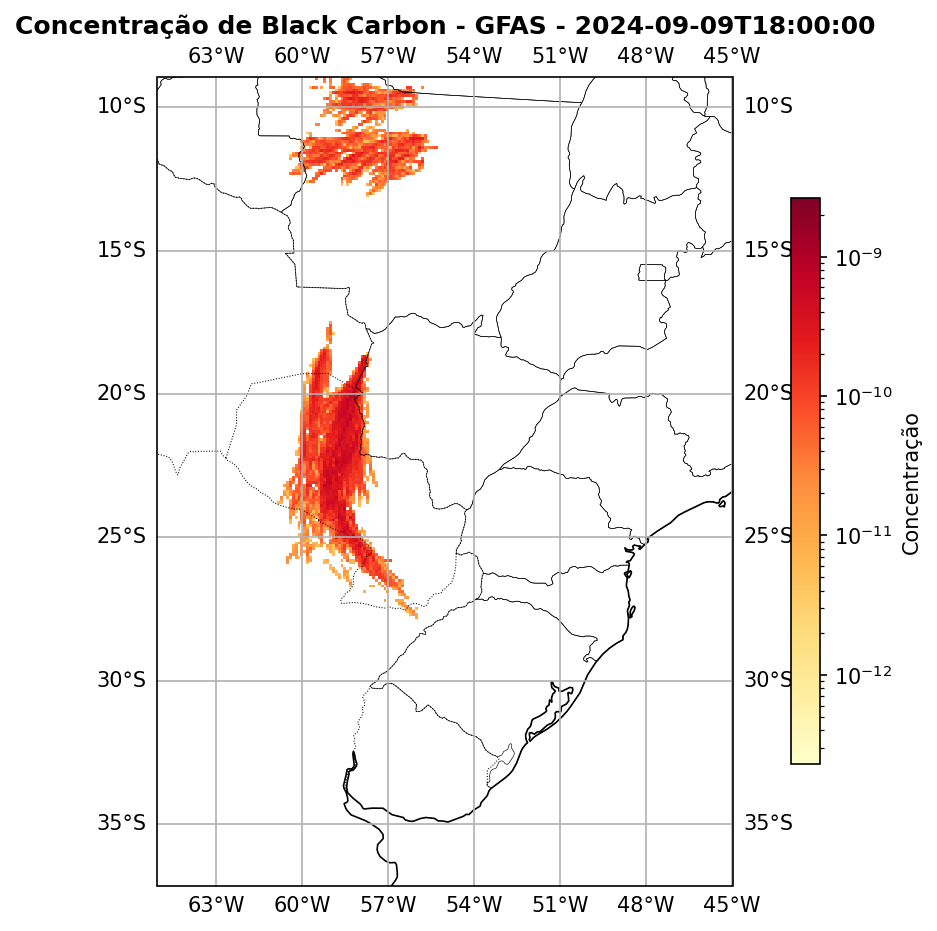
\includegraphics[width=\textwidth, trim=0cm 0cm 0cm 0.7cm, clip]{images/bc_003.png}
		\caption{2024-09-09 00:18:00}
		\label{fig:img13}
	\end{subfigure}	
	\hfill
	\begin{subfigure}[b]{0.31\textwidth}
		\centering
		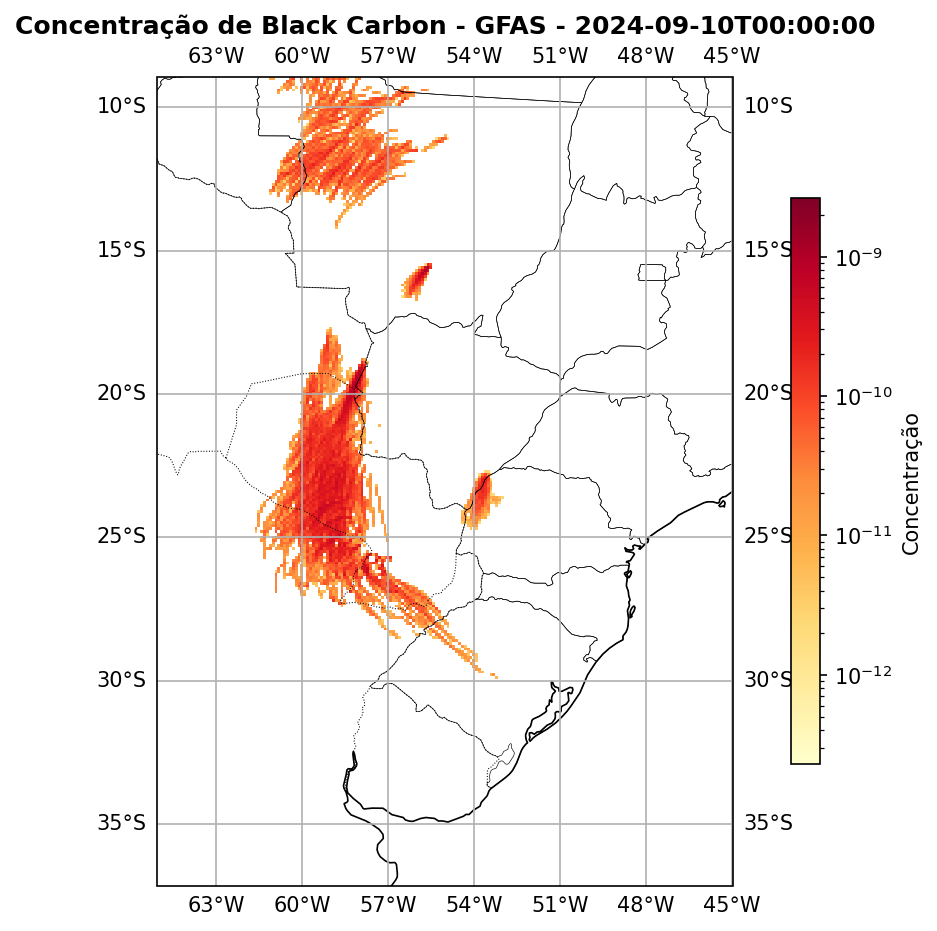
\includegraphics[width=\textwidth, trim=0cm 0cm 0cm 0.7cm, clip]{images/bc_004.png}
		\caption{2024-09-10 00:00:00}
		\label{fig:img14}
	\end{subfigure}	
	\hfill
	\begin{subfigure}[b]{0.31\textwidth}
		\centering
		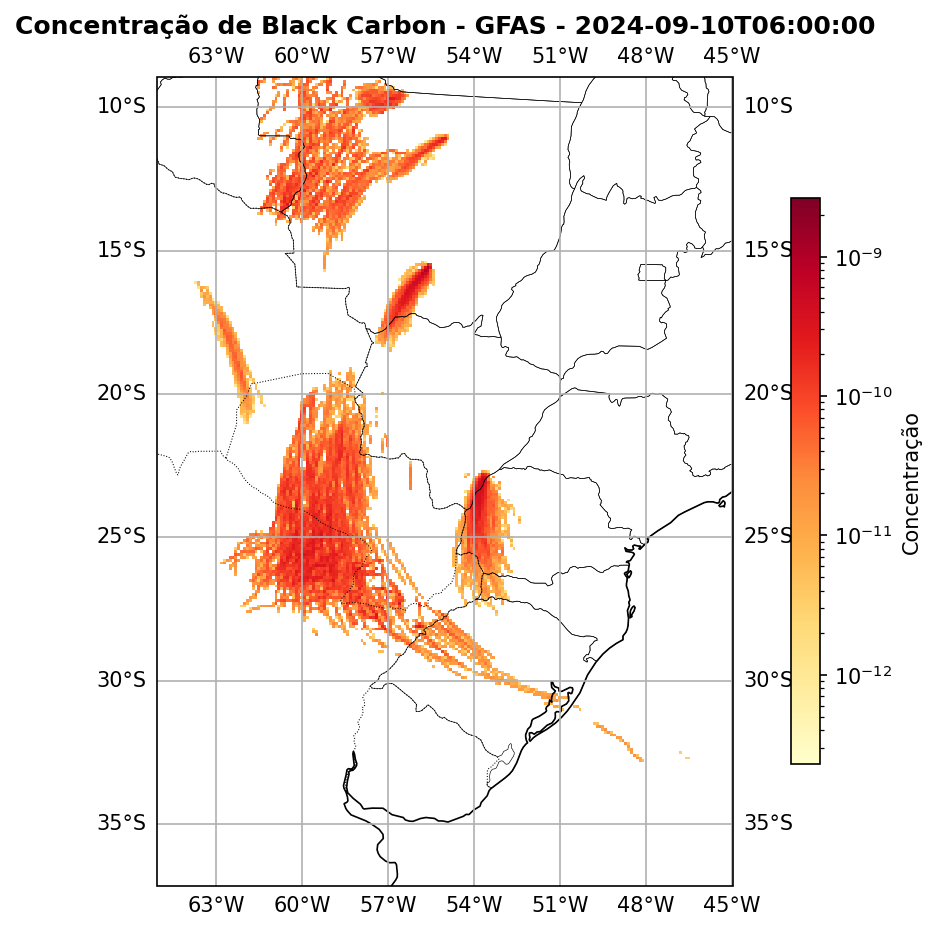
\includegraphics[width=\textwidth, trim=0cm 0cm 0cm 0.7cm, clip]{images/bc_005.png}
		\caption{2024-09-10 00:06:00}
		\label{fig:img15}
	\end{subfigure}	
	\hfill

	\vspace{0.8em} % Espaçamento vertical entre as linhas
	
	\begin{subfigure}[b]{0.31\textwidth}
		\centering
		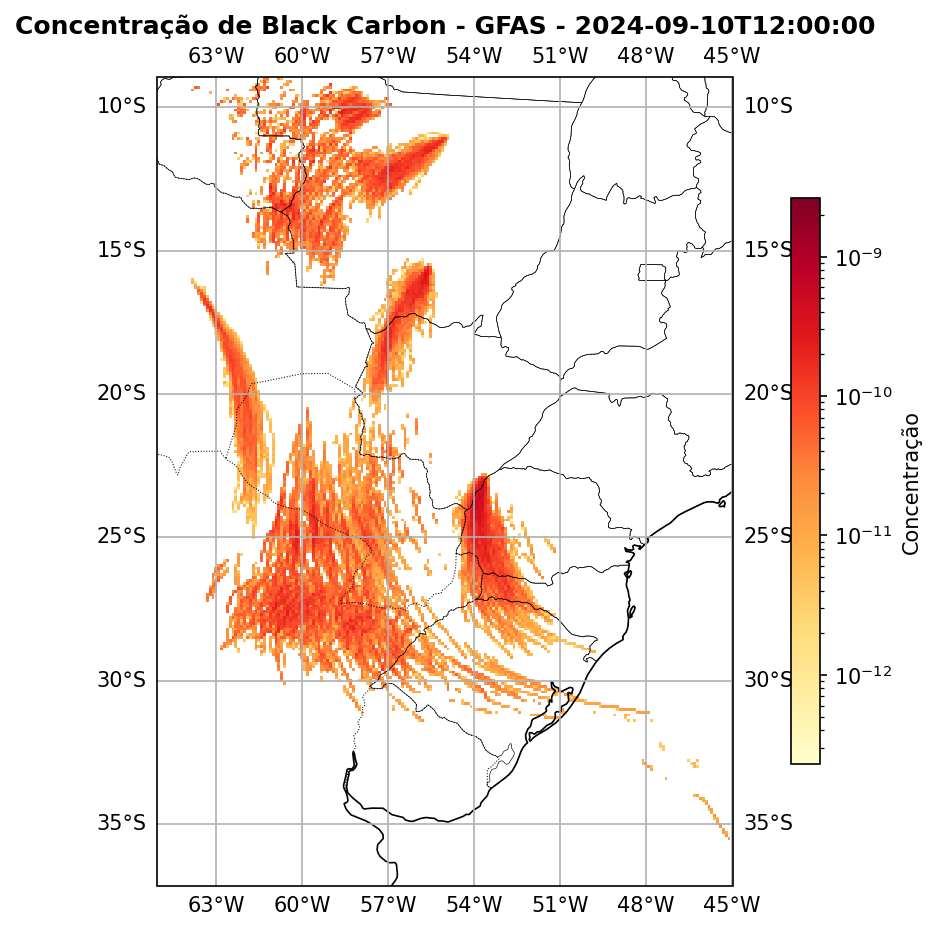
\includegraphics[width=\textwidth, trim=0cm 0cm 0cm 0.7cm, clip]{images/bc_006.png}
		\caption{2024-09-10 00:12:00}
		\label{fig:img16}
	\end{subfigure}	
	\hfill
	\begin{subfigure}[b]{0.31\textwidth}
		\centering
		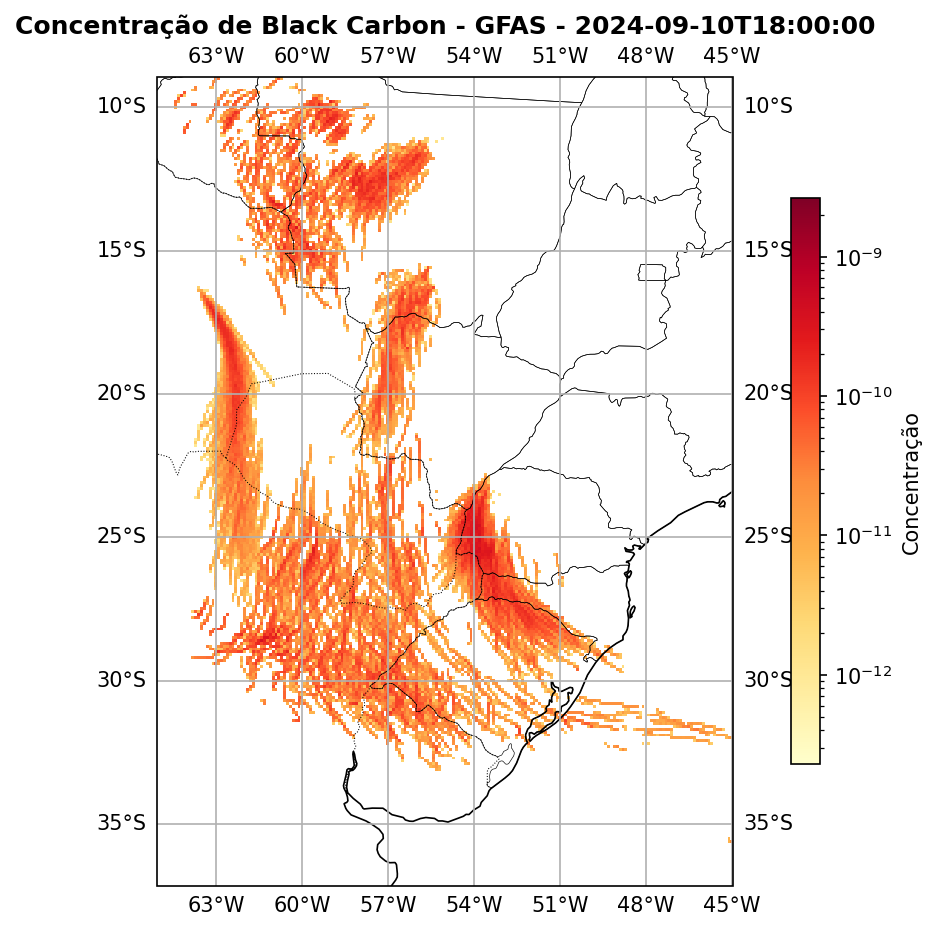
\includegraphics[width=\textwidth, trim=0cm 0cm 0cm 0.7cm, clip]{images/bc_007.png}
		\caption{2024-09-10 00:18:00}
		\label{fig:img17}
	\end{subfigure}	
	\hfill
	\begin{subfigure}[b]{0.31\textwidth}
		\centering
		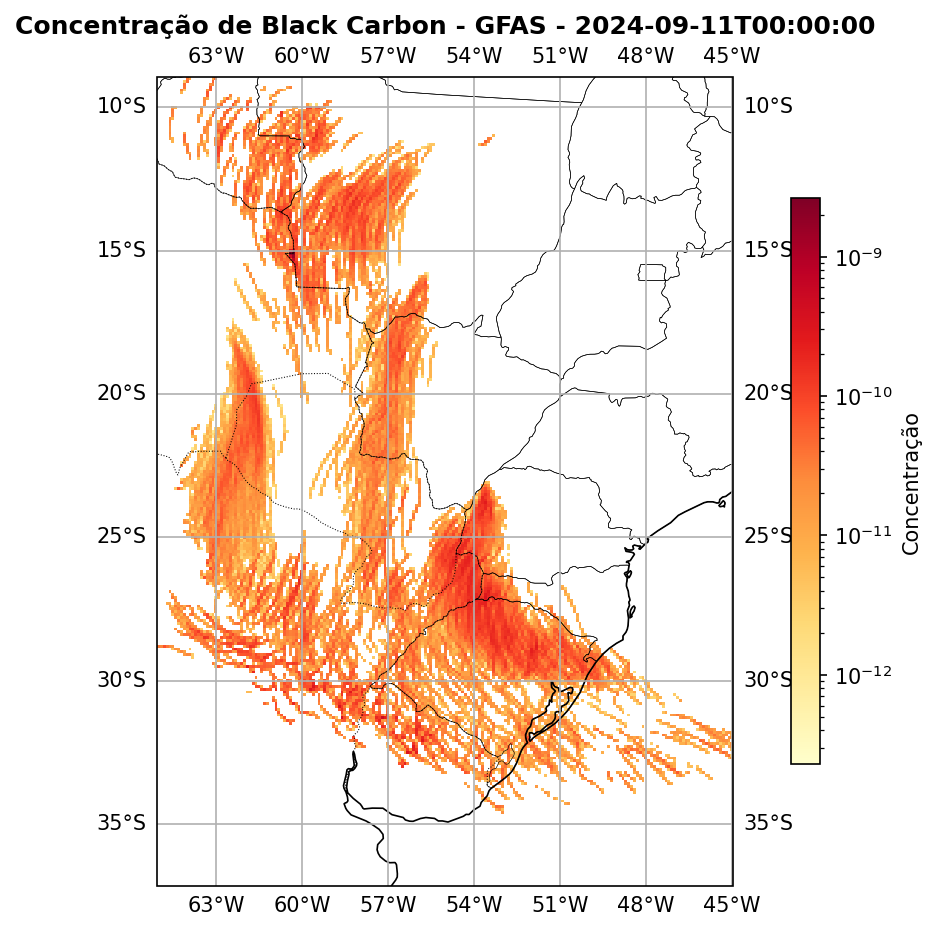
\includegraphics[width=\textwidth, trim=0cm 0cm 0cm 0.7cm, clip]{images/bc_008.png}
		\caption{2024-09-11 00:00:00}
		\label{fig:img18}
	\end{subfigure}	
	\hfill
	
	\vspace{0.8em} % Espaçamento vertical entre as linhas

	\begin{subfigure}[b]{0.31\textwidth}
		\centering
		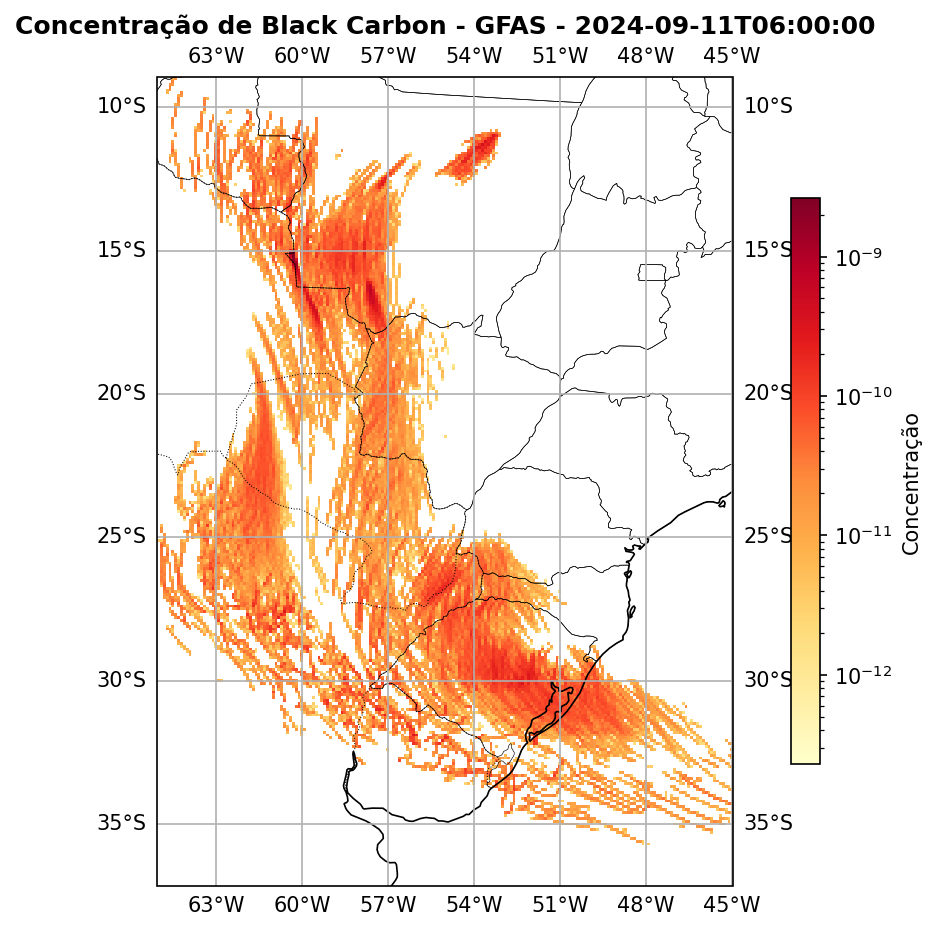
\includegraphics[width=\textwidth, trim=0cm 0cm 0cm 0.7cm, clip]{images/bc_009.png}
		\caption{2024-09-11 00:06:00}
		\label{fig:img19}
	\end{subfigure}	
	\hfill
	\begin{subfigure}[b]{0.31\textwidth}
		\centering
		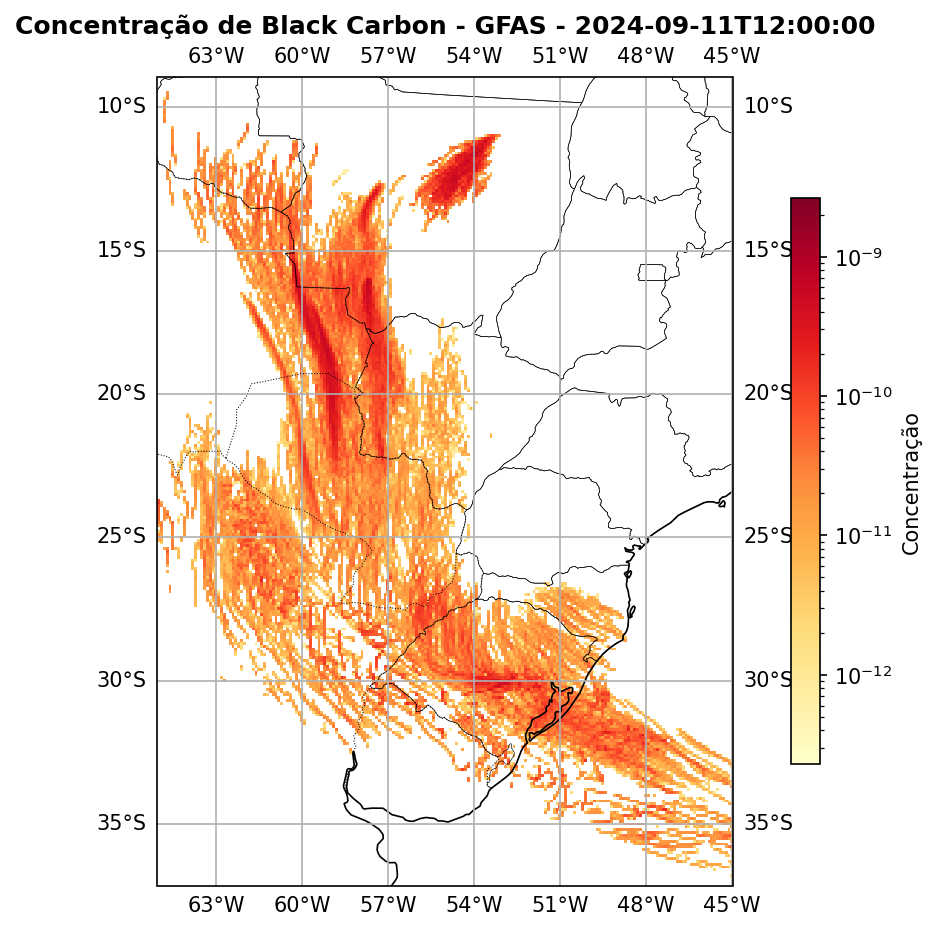
\includegraphics[width=\textwidth, trim=0cm 0cm 0cm 0.7cm, clip]{images/bc_010.png}
		\caption{2024-09-11 00:12:00}
		\label{fig:img20}
	\end{subfigure}	
	\hfill
	\begin{subfigure}[b]{0.31\textwidth}
		\centering
		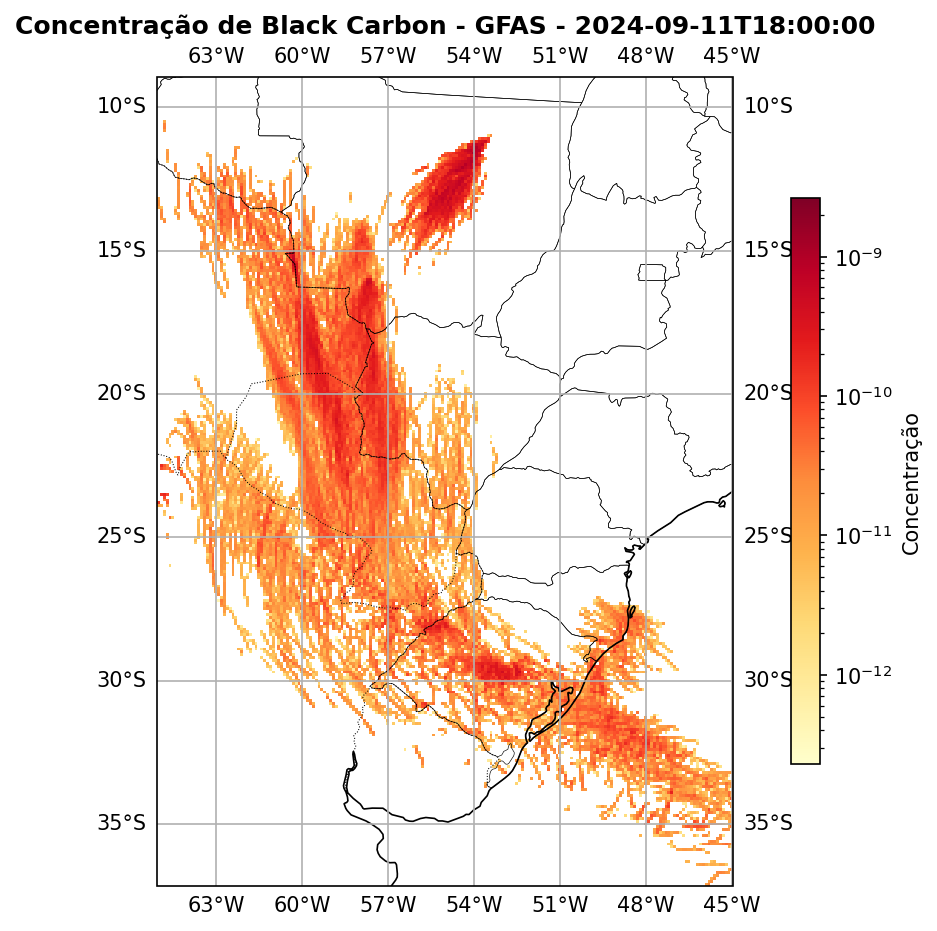
\includegraphics[width=\textwidth, trim=0cm 0cm 0cm 0.7cm, clip]{images/bc_011.png}
		\caption{2024-09-11 00:18:00}
		\label{fig:img21}
	\end{subfigure}
	\caption{Dispersão de black carbon simulada com o modelo HYSPLIT utilizando dados das reanálises ERA5 e GFAS.}
\end{figure}

\begin{figure}[htbp]
	\ContinuedFloat % Mantém a mesma numeração da figura anterior
	\centering
	
	% LINHA 5
	\begin{subfigure}[b]{0.31\textwidth}
		\centering
		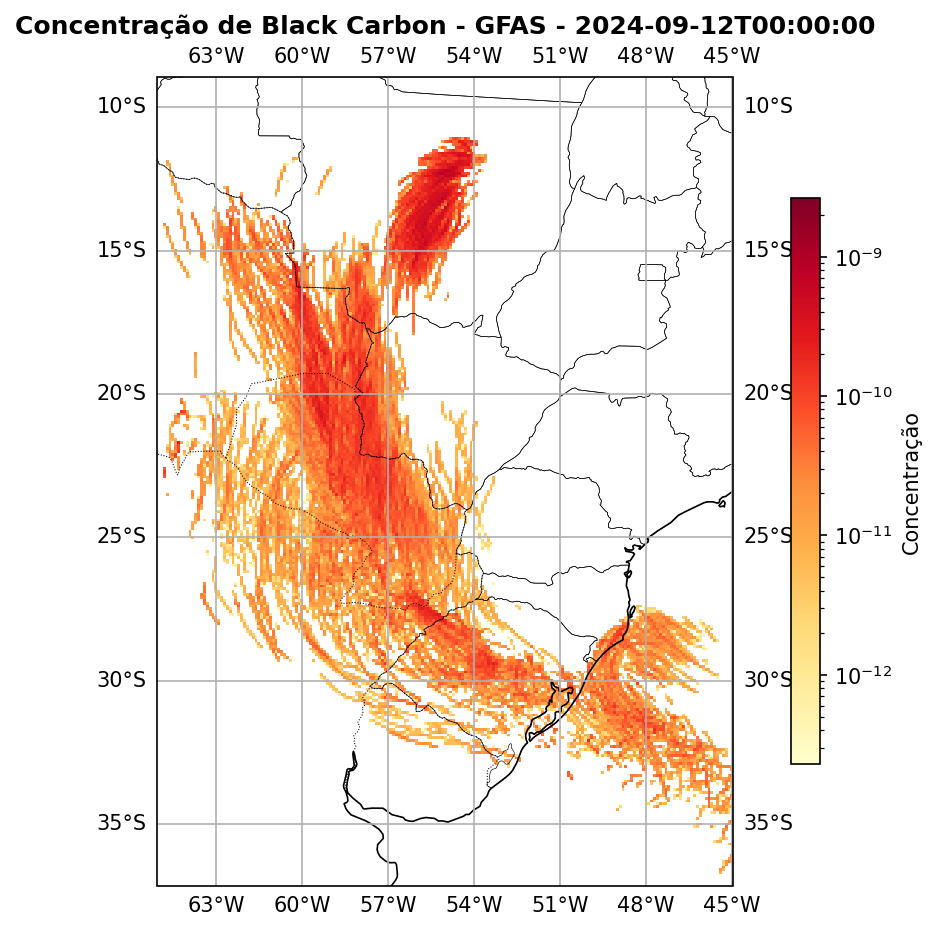
\includegraphics[width=\textwidth, trim=0cm 0cm 0cm 0.7cm, clip]{images/bc_012.png}
		\caption{2024-09-12 00:00:00}
		\label{fig:img22}
	\end{subfigure}    
	\hfill
	\begin{subfigure}[b]{0.31\textwidth}
		\centering
		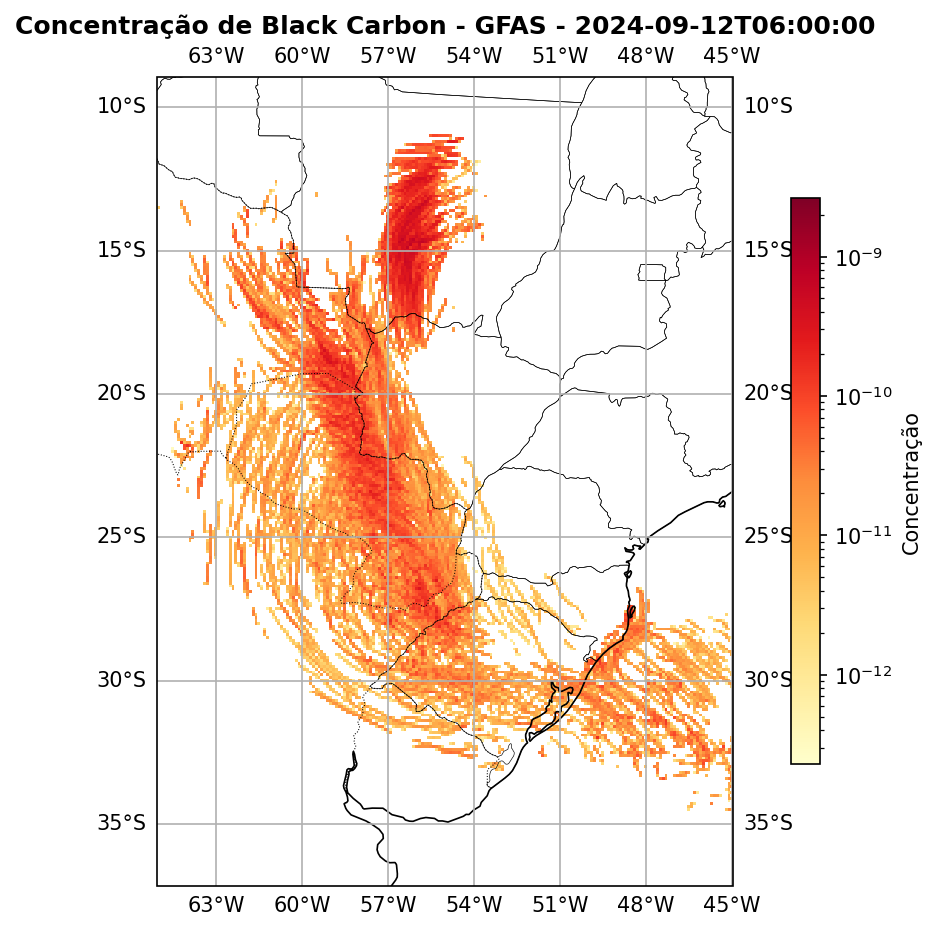
\includegraphics[width=\textwidth, trim=0cm 0cm 0cm 0.7cm, clip]{images/bc_013.png}
		\caption{2024-09-12 00:06:00}
		\label{fig:img23}
	\end{subfigure}    
	\hfill
	\begin{subfigure}[b]{0.31\textwidth}
		\centering
		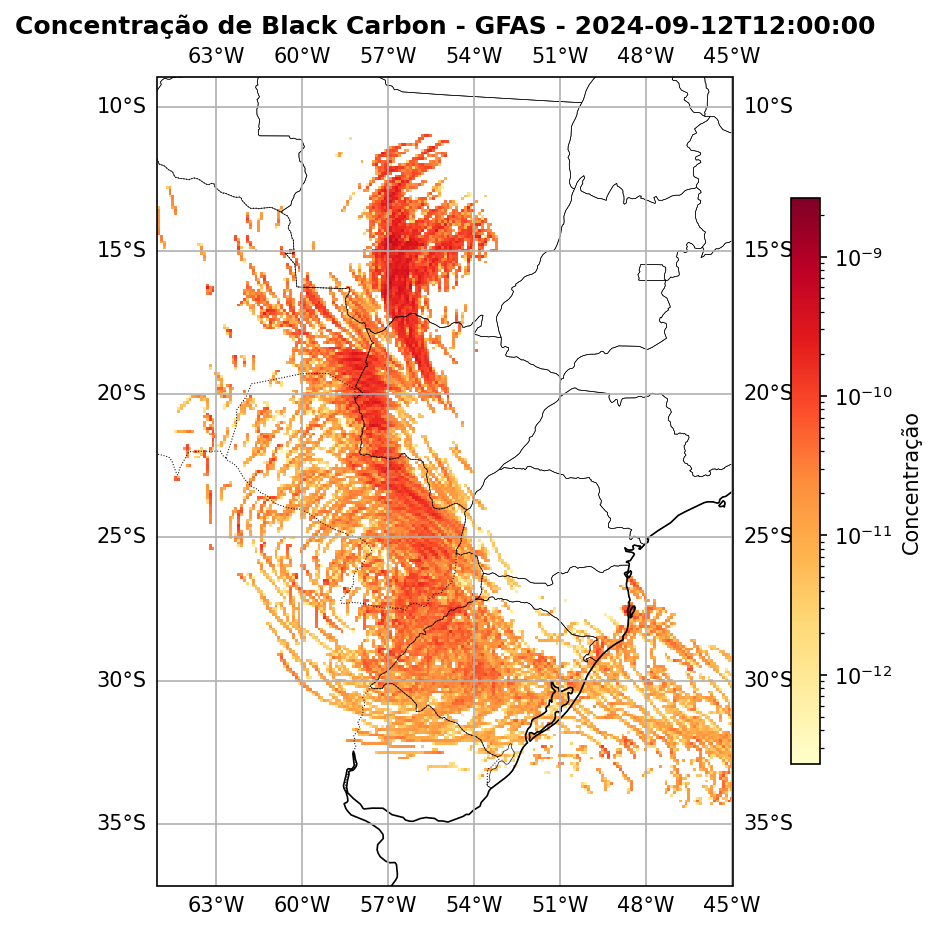
\includegraphics[width=\textwidth, trim=0cm 0cm 0cm 0.7cm, clip]{images/bc_014.png}
		\caption{2024-09-12 00:12:00}
		\label{fig:img24}
	\end{subfigure}    
	
	\vspace{0.8em}
	
	% LINHA 6
	\begin{subfigure}[b]{0.31\textwidth}
		\centering
		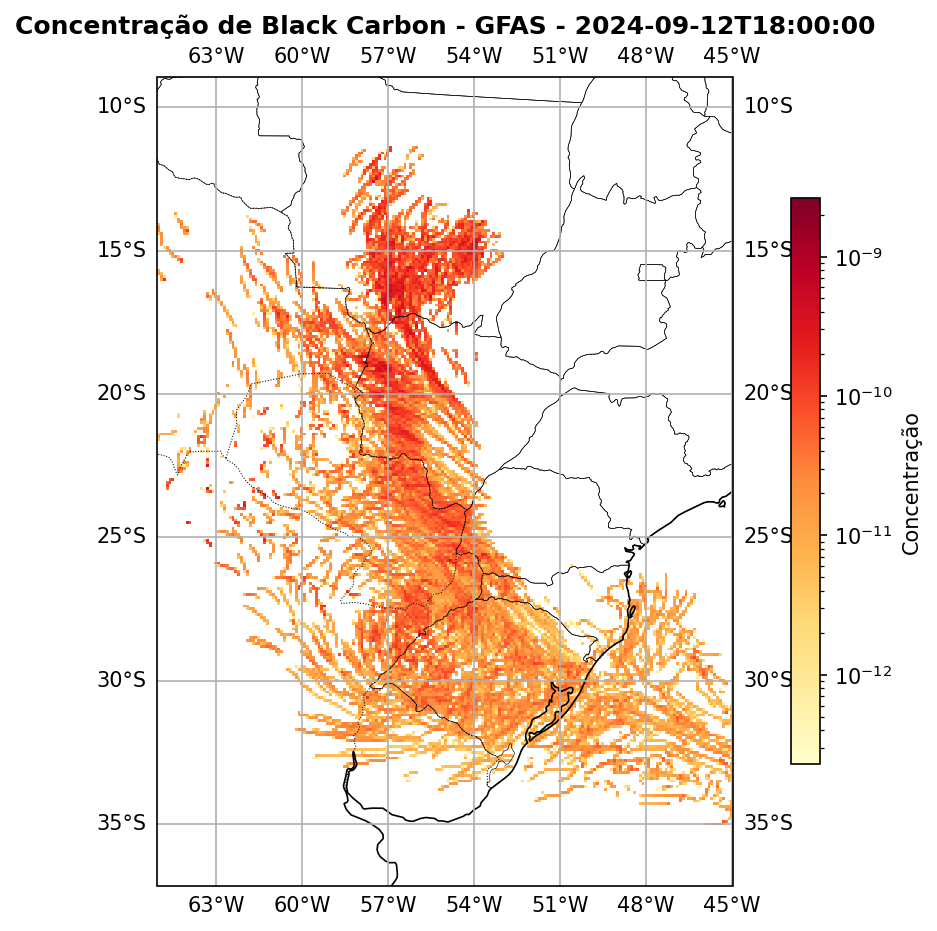
\includegraphics[width=\textwidth, trim=0cm 0cm 0cm 0.7cm, clip]{images/bc_015.png}
		\caption{2024-09-12 00:18:00}
		\label{fig:img25}
	\end{subfigure}
	
		\caption{Dispersão de black carbon simulada com o modelo HYSPLIT utilizando dados das reanálises ERA5 e GFAS. (continuação).} % Opcional
\end{figure}



\begin{figure}[htbp]
	\centering
	% --- LINHA 1 ---
	\begin{subfigure}[b]{0.31\textwidth}
		\centering
		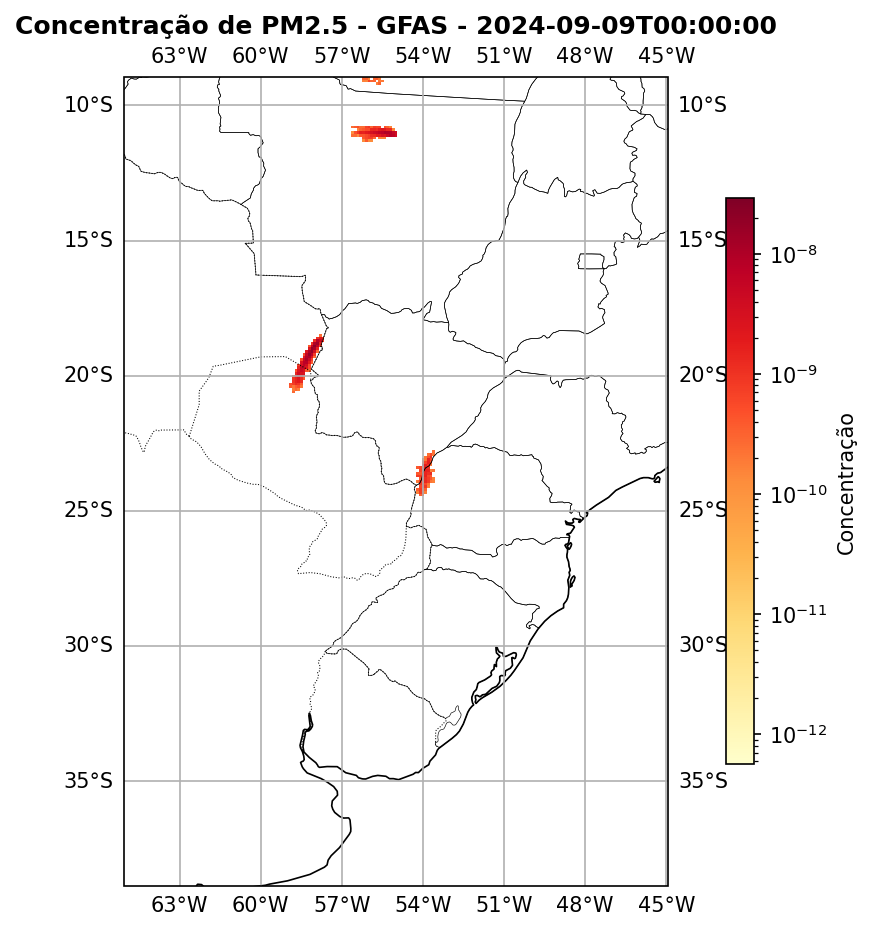
\includegraphics[width=\textwidth, trim=0cm 0cm 0cm 0.7cm, clip]{images/pm25_000.png}
		\caption{2024-09-09 00:00:00}
		\label{fig:img26}
	\end{subfigure}
	\hfill
	\begin{subfigure}[b]{0.31\textwidth}
		\centering
		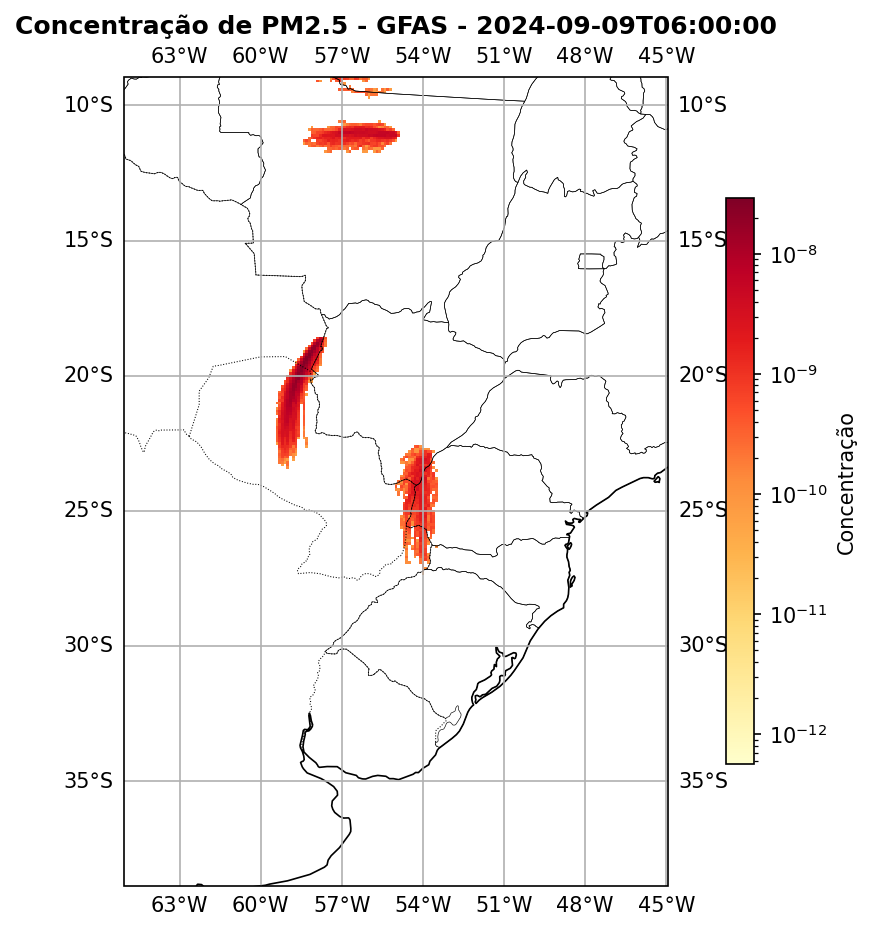
\includegraphics[width=\textwidth, trim=0cm 0cm 0cm 0.7cm, clip]{images/pm25_001.png}
		\caption{2024-09-09 00:06:00}
		\label{fig:img27}
	\end{subfigure}
	\hfill
	\begin{subfigure}[b]{0.31\textwidth}
		\centering
		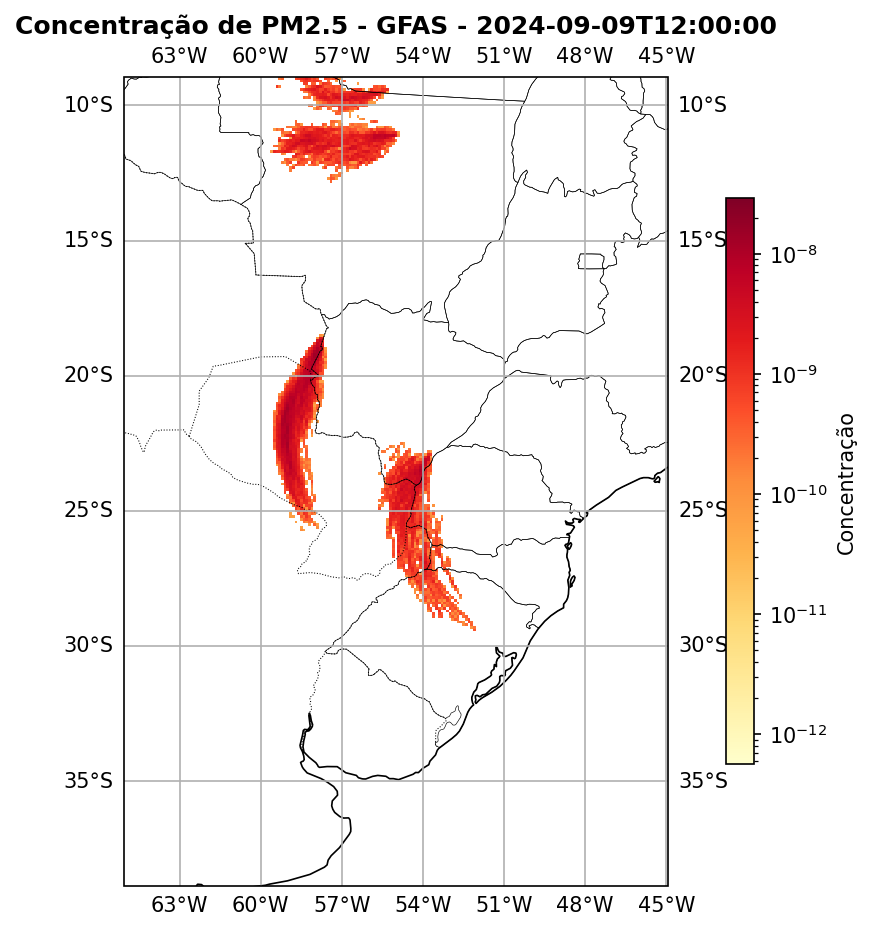
\includegraphics[width=\textwidth, trim=0cm 0cm 0cm 0.7cm, clip]{images/pm25_002.png}
		\caption{2024-09-09 00:12:00}
		\label{fig:img28}
	\end{subfigure}
	\hfill
	
	\vspace{0.8em} % Espaçamento vertical entre as linhas
	
	\begin{subfigure}[b]{0.31\textwidth}
		\centering
		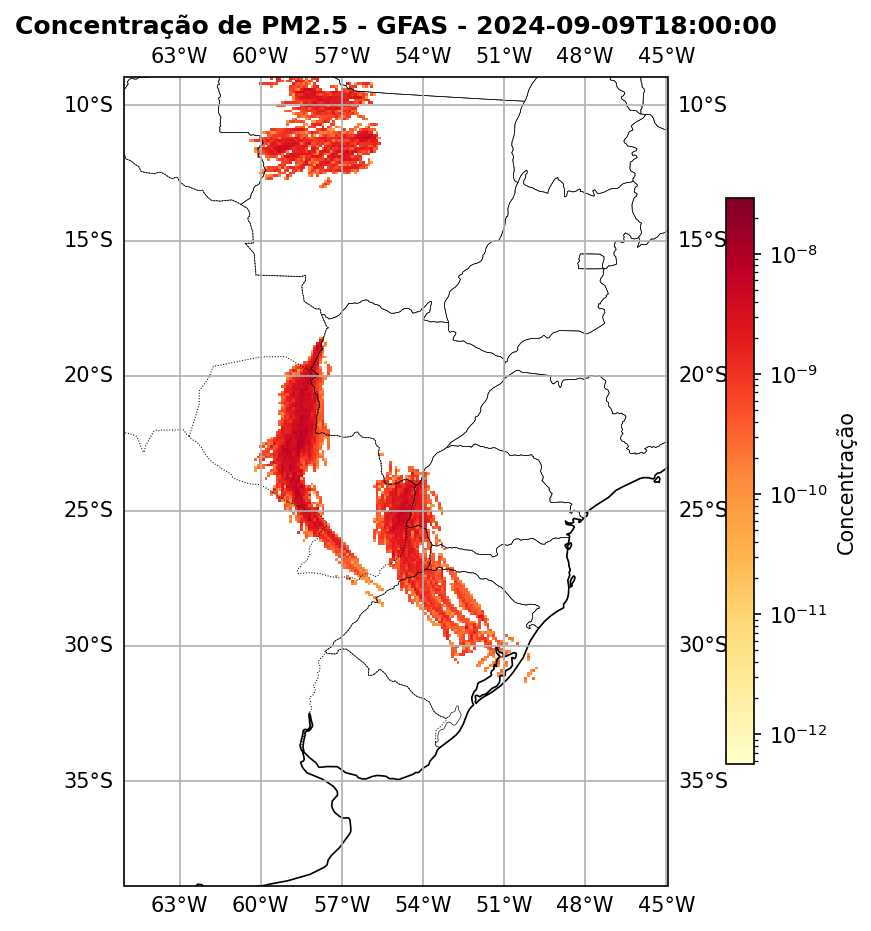
\includegraphics[width=\textwidth, trim=0cm 0cm 0cm 0.7cm, clip]{images/pm25_003.png}
		\caption{2024-09-09 00:18:00}
		\label{fig:img29}
	\end{subfigure}	
	\hfill
	\begin{subfigure}[b]{0.31\textwidth}
		\centering
		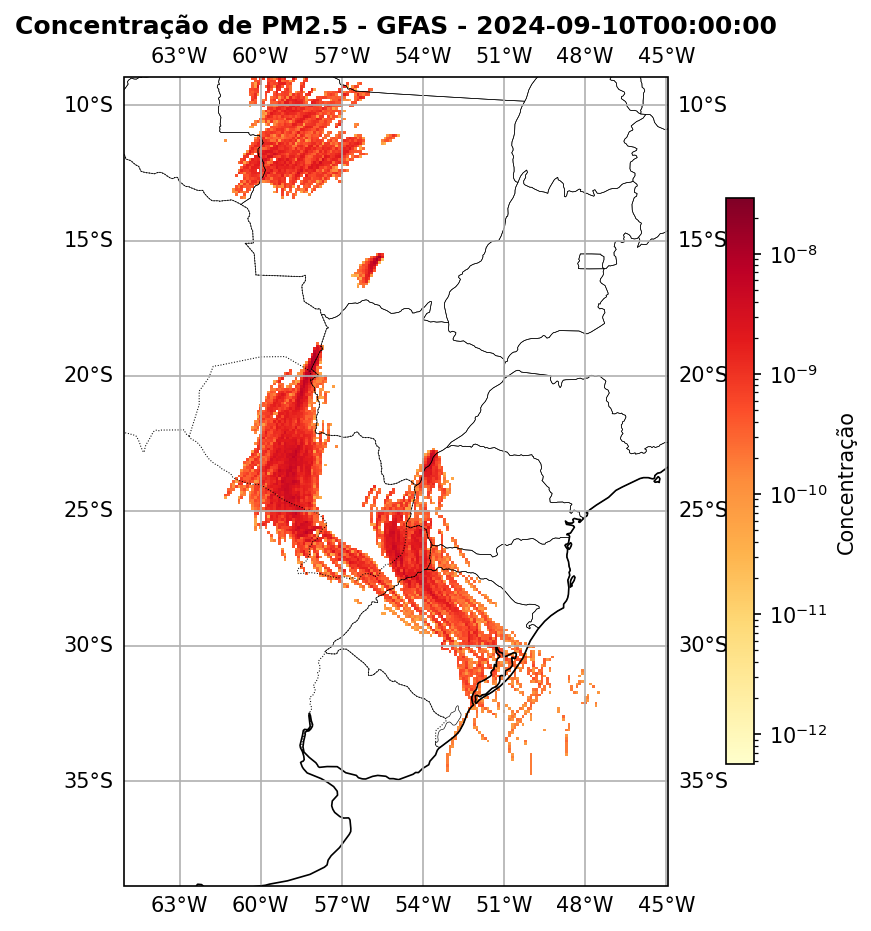
\includegraphics[width=\textwidth, trim=0cm 0cm 0cm 0.7cm, clip]{images/pm25_004.png}
		\caption{2024-09-10 00:00:00}
		\label{fig:img30}
	\end{subfigure}	
	\hfill
	\begin{subfigure}[b]{0.31\textwidth}
		\centering
		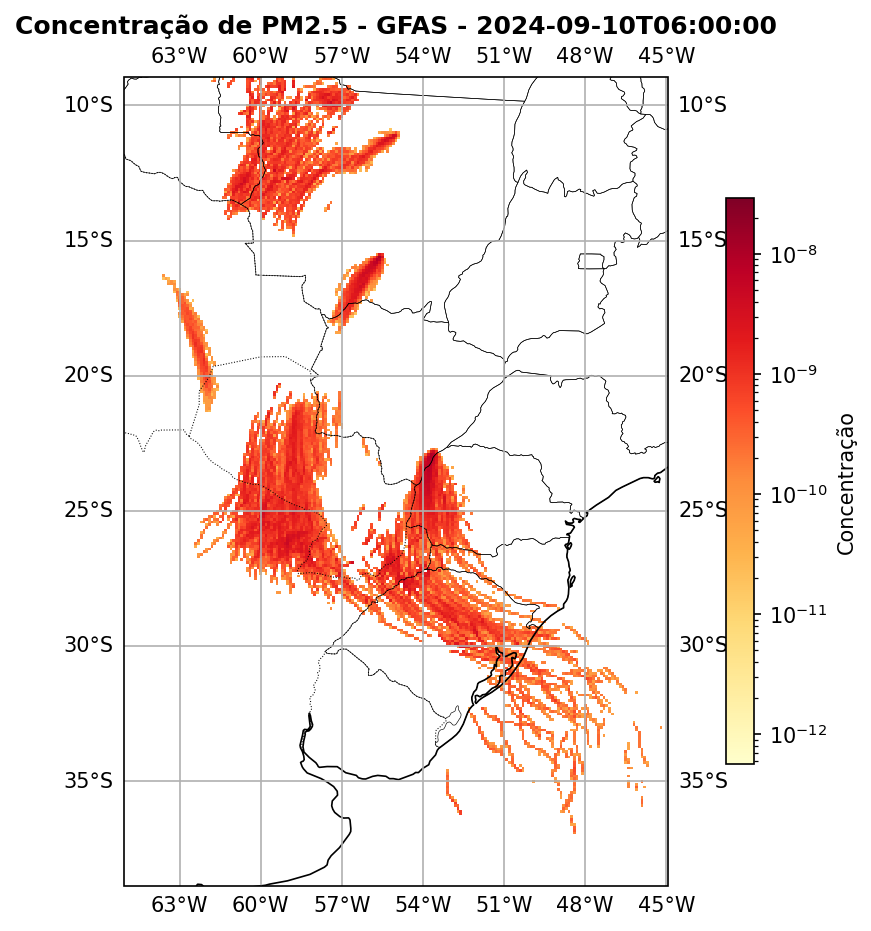
\includegraphics[width=\textwidth, trim=0cm 0cm 0cm 0.7cm, clip]{images/pm25_005.png}
		\caption{2024-09-10 00:06:00}
		\label{fig:img31}
	\end{subfigure}	
	\hfill
	
	\vspace{0.8em} % Espaçamento vertical entre as linhas
	
	\begin{subfigure}[b]{0.31\textwidth}
		\centering
		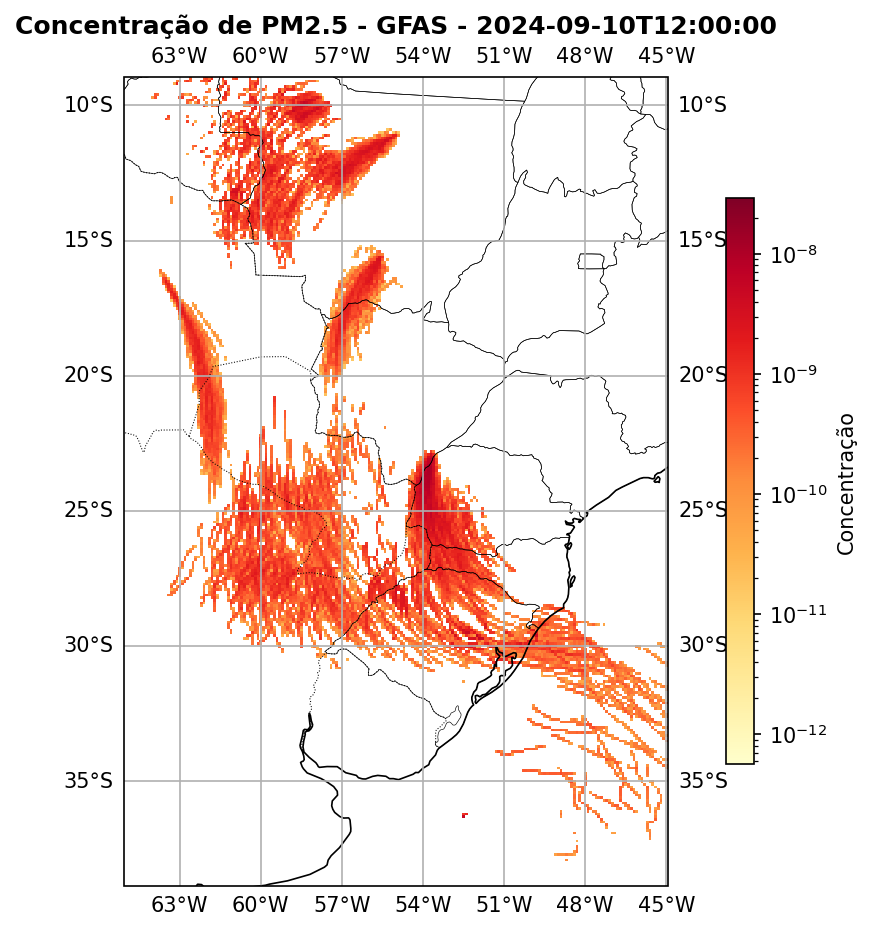
\includegraphics[width=\textwidth, trim=0cm 0cm 0cm 0.7cm, clip]{images/pm25_006.png}
		\caption{2024-09-10 00:12:00}
		\label{fig:img32}
	\end{subfigure}	
	\hfill
	\begin{subfigure}[b]{0.31\textwidth}
		\centering
		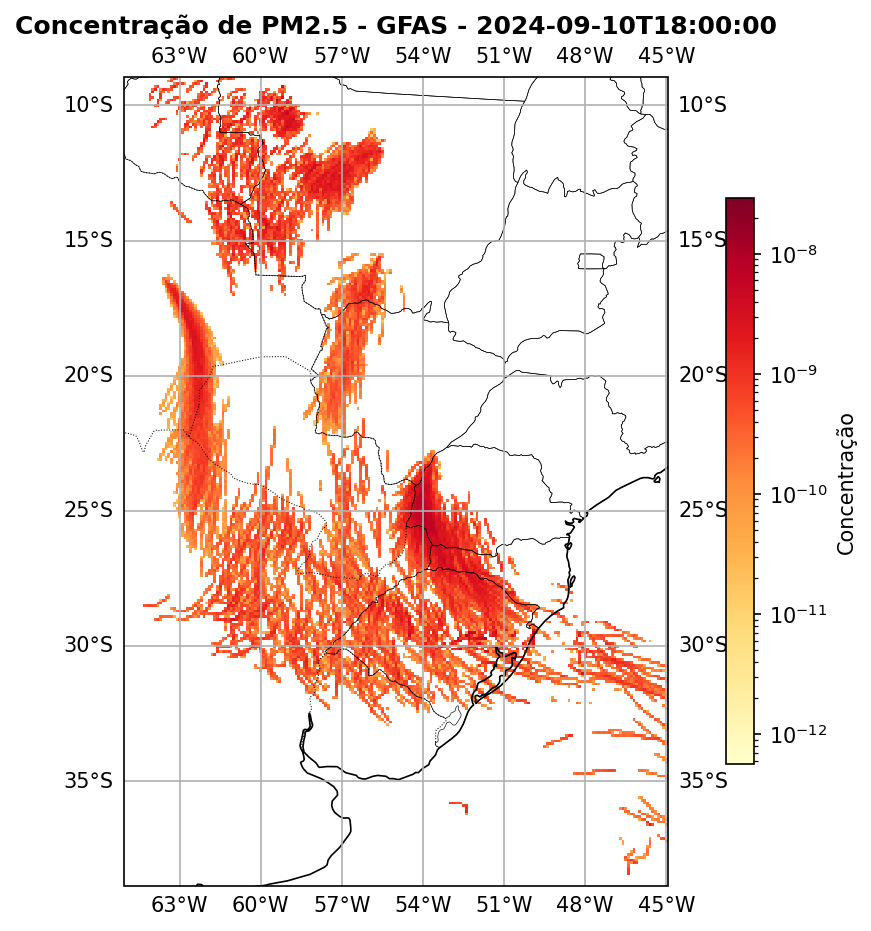
\includegraphics[width=\textwidth, trim=0cm 0cm 0cm 0.7cm, clip]{images/pm25_007.png}
		\caption{2024-09-10 00:18:00}
		\label{fig:img33}
	\end{subfigure}	
	\hfill
	\begin{subfigure}[b]{0.31\textwidth}
		\centering
		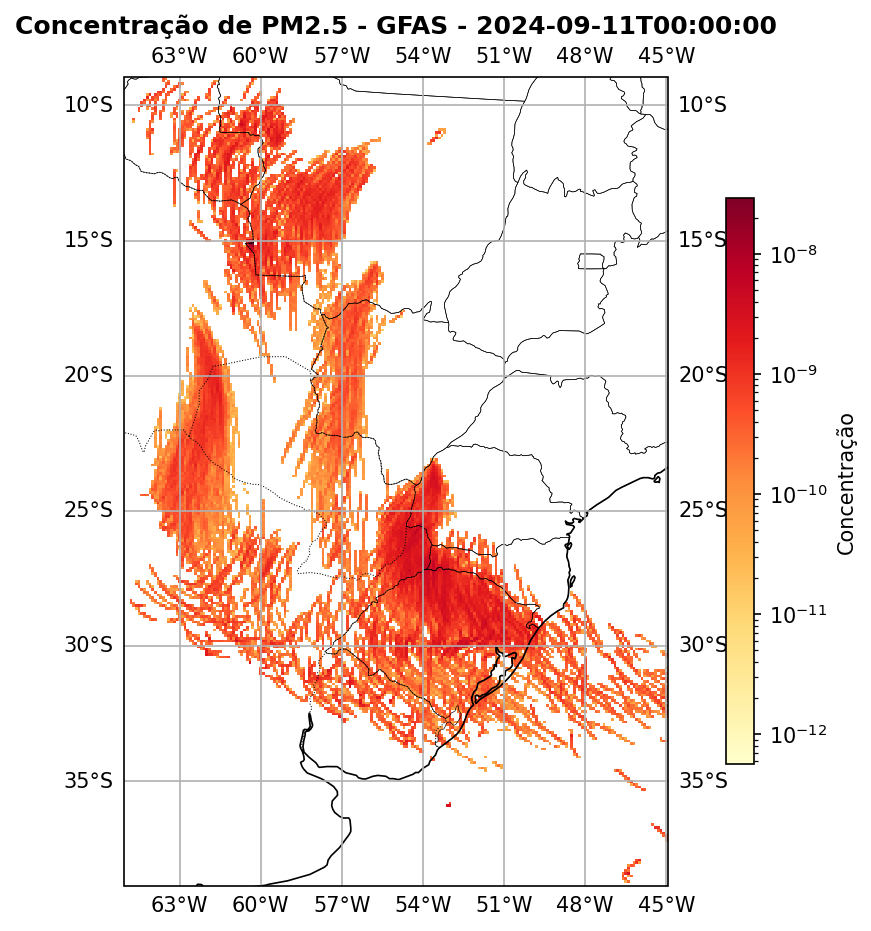
\includegraphics[width=\textwidth, trim=0cm 0cm 0cm 0.7cm, clip]{images/pm25_008.png}
		\caption{2024-09-11 00:00:00}
		\label{fig:img34}
	\end{subfigure}	
	\hfill
	
	\vspace{0.8em} % Espaçamento vertical entre as linhas
	
	\begin{subfigure}[b]{0.31\textwidth}
		\centering
		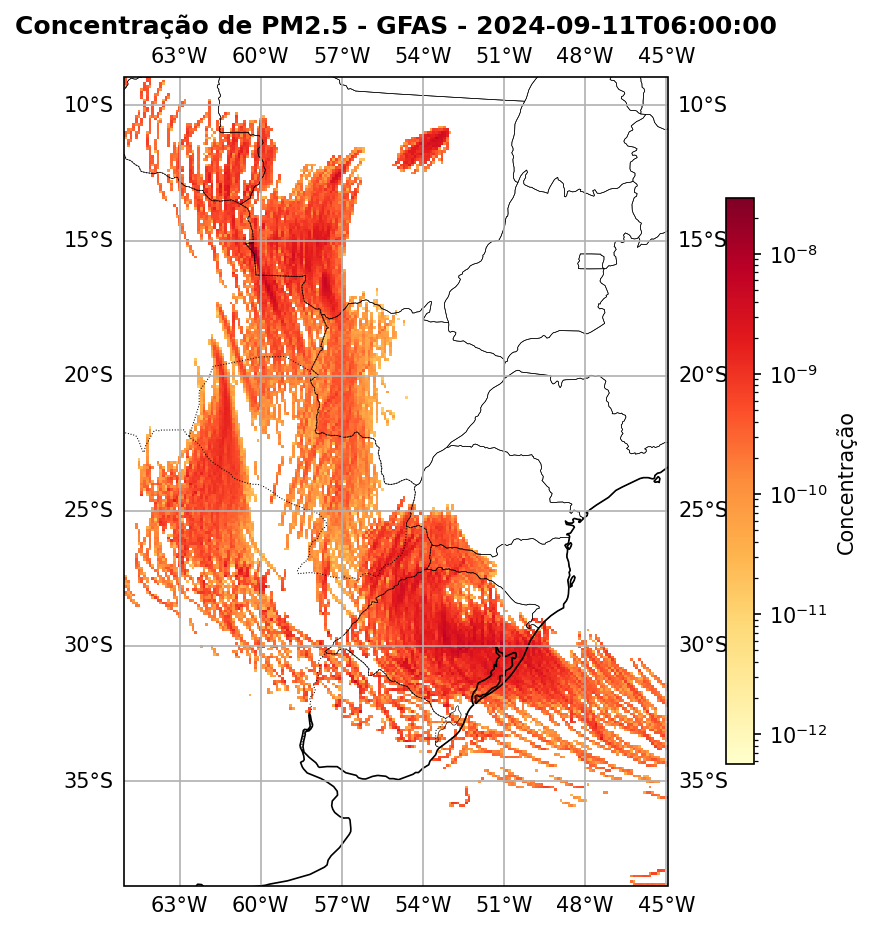
\includegraphics[width=\textwidth, trim=0cm 0cm 0cm 0.7cm, clip]{images/pm25_009.png}
		\caption{2024-09-11 00:06:00}
		\label{fig:img35}
	\end{subfigure}	
	\hfill
	\begin{subfigure}[b]{0.31\textwidth}
		\centering
		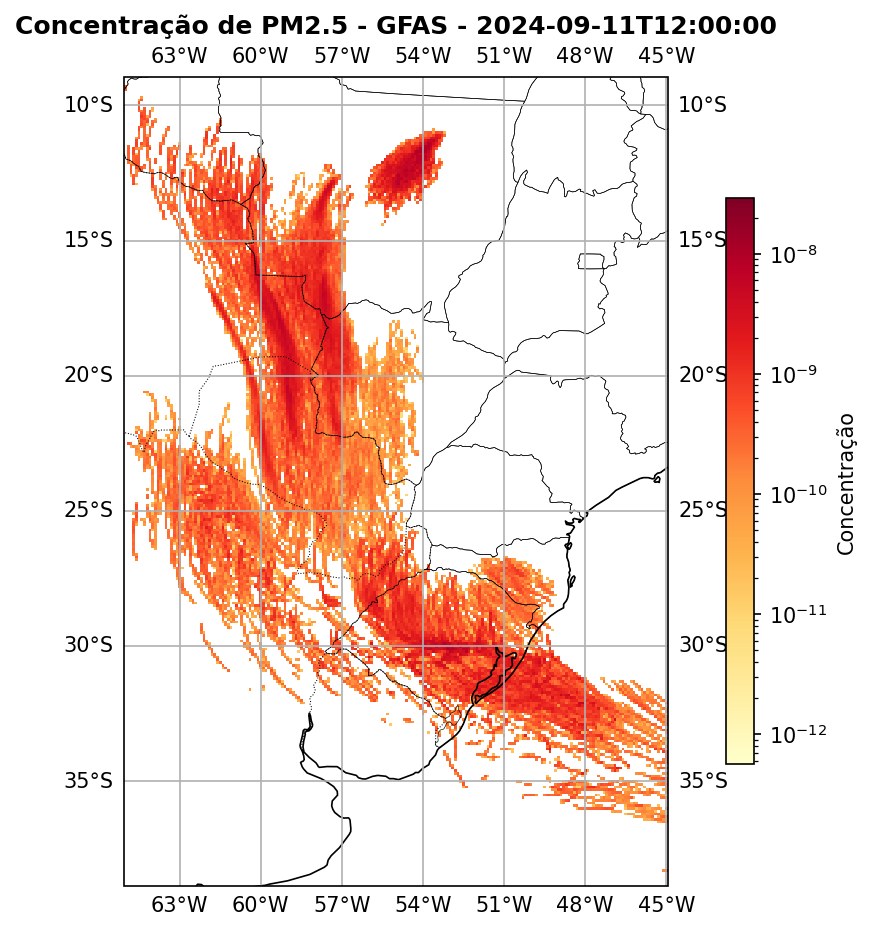
\includegraphics[width=\textwidth, trim=0cm 0cm 0cm 0.7cm, clip]{images/pm25_010.png}
		\caption{2024-09-11 00:12:00}
		\label{fig:img36}
	\end{subfigure}	
	\hfill
	\begin{subfigure}[b]{0.31\textwidth}
		\centering
		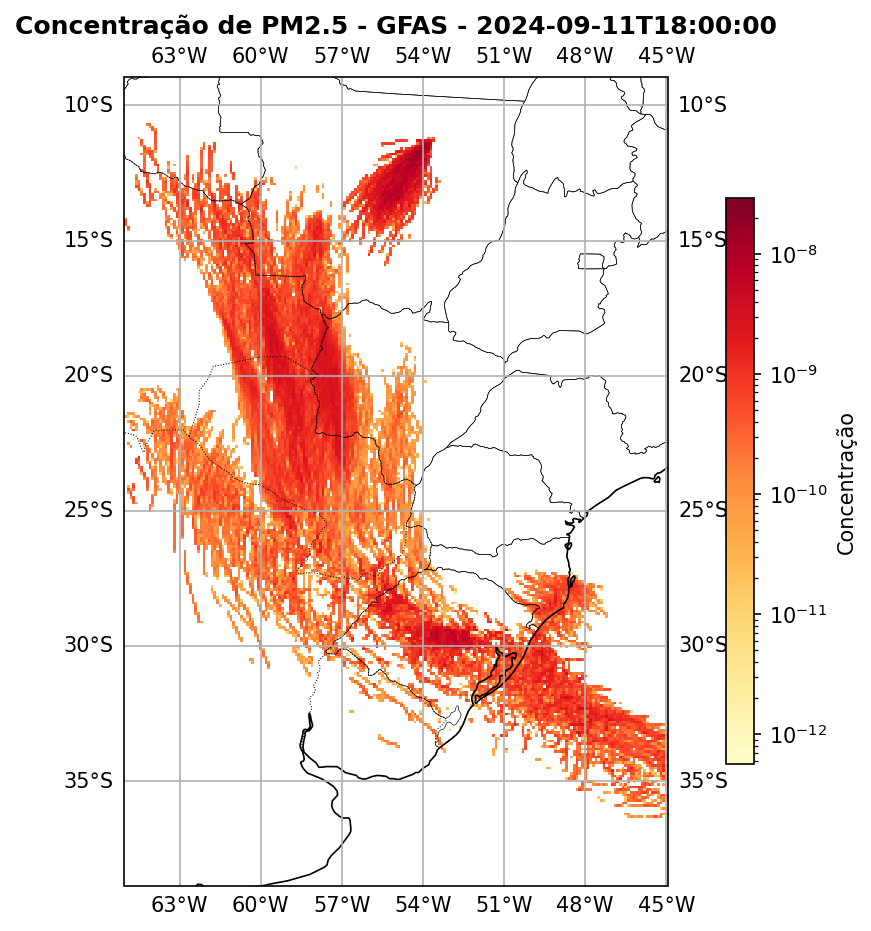
\includegraphics[width=\textwidth, trim=0cm 0cm 0cm 0.7cm, clip]{images/pm25_011.png}
		\caption{2024-09-11 00:18:00}
		\label{fig:img37}
	\end{subfigure}
	\caption{Dispersão de PM2.5 simulada com o modelo HYSPLIT utilizando dados das reanálises ERA5 e GFAS.}
\end{figure}

\begin{figure}[htbp]
	\ContinuedFloat % Mantém a mesma numeração da figura anterior
	\centering
	
	% LINHA 5
	\begin{subfigure}[b]{0.31\textwidth}
		\centering
		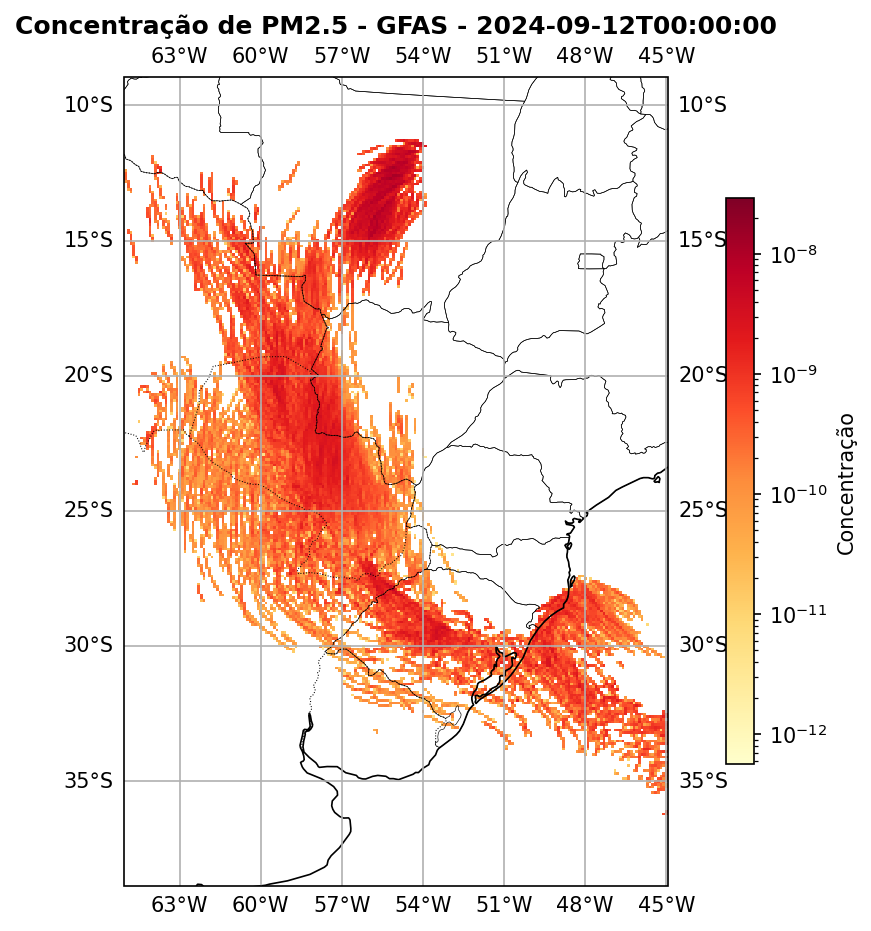
\includegraphics[width=\textwidth, trim=0cm 0cm 0cm 0.7cm, clip]{images/pm25_012.png}
		\caption{2024-09-12 00:00:00}
		\label{fig:img38}
	\end{subfigure}    
	\hfill
	\begin{subfigure}[b]{0.31\textwidth}
		\centering
		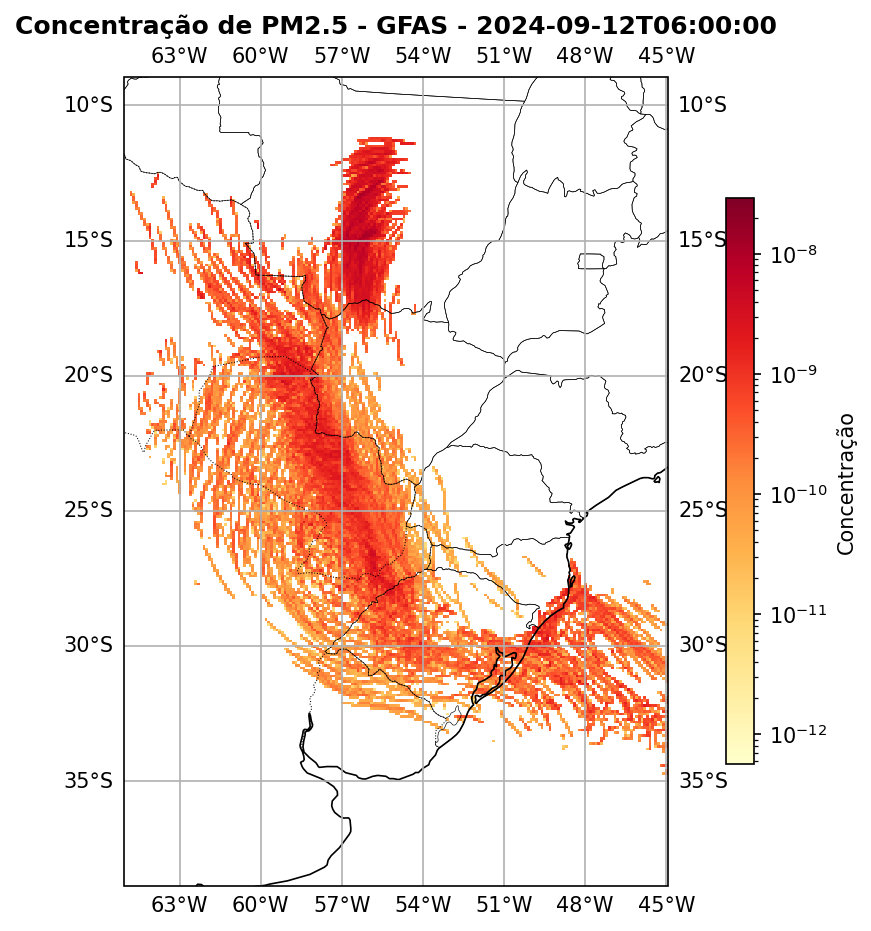
\includegraphics[width=\textwidth, trim=0cm 0cm 0cm 0.7cm, clip]{images/pm25_013.png}
		\caption{2024-09-12 00:06:00}
		\label{fig:img39}
	\end{subfigure}    
	\hfill
	\begin{subfigure}[b]{0.31\textwidth}
		\centering
		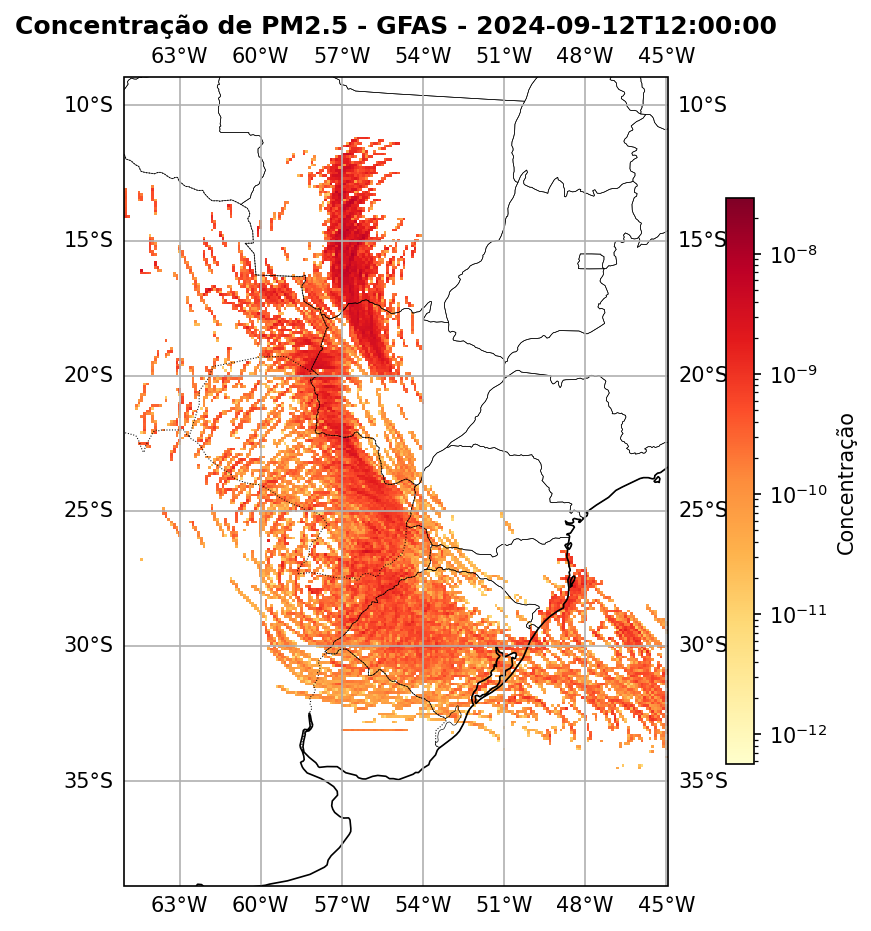
\includegraphics[width=\textwidth, trim=0cm 0cm 0cm 0.7cm, clip]{images/pm25_014.png}
		\caption{2024-09-12 00:12:00}
		\label{fig:img40}
	\end{subfigure}    
	
	\vspace{0.8em}
	
	% LINHA 6
	\begin{subfigure}[b]{0.31\textwidth}
		\centering
		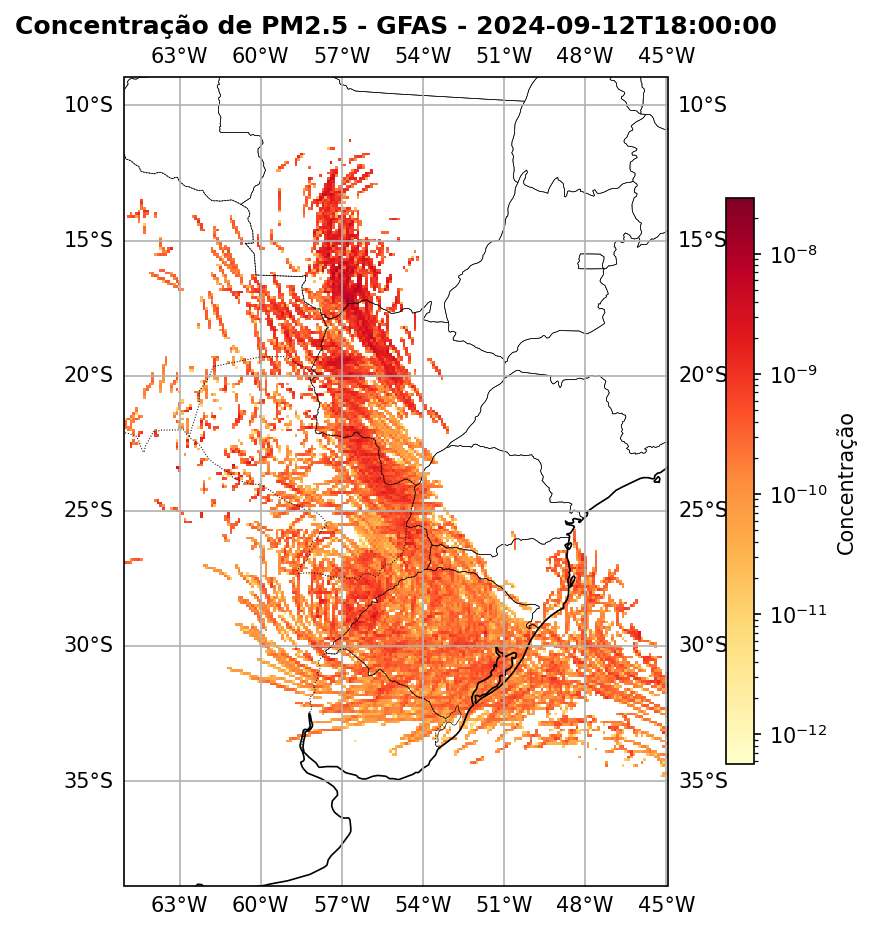
\includegraphics[width=\textwidth, trim=0cm 0cm 0cm 0.7cm, clip]{images/pm25_015.png}
		\caption{2024-09-12 00:18:00}
		\label{fig:img41}
	\end{subfigure}
	
	\caption{Dispersão de PM2.5 simulada com o modelo HYSPLIT utilizando dados das reanálises ERA5 e GFAS. (continuação).} % Opcional
\end{figure}



